\documentclass[11pt]{report}              % Book class in 11 points
\ifdefined\HCode
\usepackage{tex4ht}
\else
\usepackage{mcs_pack}
\fi
\usepackage{chngcntr}


%begin      p. fischer
\def\ds{\displaystyle}
\def\d{\partial}
\def\dO{\partial \Omega}
\def\dOt{\tilde {\partial \Omega}}
\def\spn{ {\textstyle span} \{ }
\def\ee{{\hat {\underline e}}}
\def\uxh{{\hat {\underline x}}}
\def\eq{ \; = \; }
%\def\eqq{ \, \equiv \, }
\def\eqq{ \, := \, }
% \def\es{ \, = \, }
\def\es{ = }
\def\ea{ \; & = & \; }
\def\sp{ \; + \; }
\def\sm{ \; - \; }
\def\ds{ \Delta s }
\def\dt{ \Delta t }
\def\dx{ \Delta x }
\def\XX{\raisebox{0.3ex}{$\chi$}}
\def\cW{{\cal W}}
\def\cL{{\cal L}}
\def\cB{{\cal B}}
\def\cH{{\cal H}}
\def\cI{{\cal I}}
\def\cM{{\cal M}}
\def\cN{{\cal N}}
\def\No{{N_o}}
\def\cR{{\cal R}}
\def\scriptO{{{\it O}\kern -.42em {\it `}\kern + .20em}}
\def\RR{{{\rm l}\kern - .15em {\rm R} }}
\def\PP{{{\rm l}\kern - .15em {\rm P} }}
%\def\L2{{{\cal L}^2}}
%\def\H1{{{\cal H}^1}}
%\def\L2{{{\bf L}^2}}
%\def\H1{{{\bf H}^1}}
\def\L2{{{\sf L}^2}}
\def\H1{{{\sf H}^1}}
\def\PN2{{\PP_{N}-\PP_{N-2}}}
\def\PNK{{\PP_{N,K}(\Omega)}}
\def\complex{{{\rm C} \kern - .53em {\rm l} \kern + .38em}}
\def\eop{\hbox{\vrule width 6pt height 6pt depth 0pt}}

\def\am{{ | \lambda_{\max} |}}
\def\a1{{ | \lambda_{\min} |}}
\def\lm{{   \lambda_{\max}  }}
\def\l1{{   \lambda_{\min}  }}
\def\bhu{{\hat   {\bf u}}}

\def\bff{{\bf f}}
\def\tp {{\tilde p}}
\def\btu{{\tilde {\bf u}}}
\def\utU{{\underline {\tilde {\bf u}}}}
\def\uU{{{\underline {\bf u}}}}
\def\bhu{{\hat   {\bf u}}}
\def\bhn{{\hat   {\bf n}}}
\def\ugt{{\tilde {\underline g}}}
\def\uut{{\tilde {\underline u}}}
\def\uxt{{\tilde {\underline x}}}
\def\ubt{{\tilde {\underline b}}}
\def\bue{{\underline {\bf e}}}
\def\bur{{\underline {\bf r}}}
\def\bu0{{\underline {\bf 0}}}
\def\buu{{\underline {\bf u}}}
\def\buf{{\underline {\bf f}}}
\def\br{{\bf r}}
\def\bn{{\bf n}}
\def\bc{{\bf c}}
\def\bu{{\bf u}}
\def\bv{{\bf v}}
\def\bx{{\bf x}}
\def\bxt{{\tilde {\bf x}}}
\def\bA{{\bf A}}
\def\bX{{\bf X}}
\def\bB{{\bf B}}
\def\bD{{\bf D}}
\def\bH{{\bf H}}
\def\bI{{\bf I}}
\def\bQ{{\bf Q}}

\def\At{{\tilde A}}
\def\Bt{{\tilde B}}
\def\Bb{{\bar B}}
\def\Dt{{\tilde D}}
\def\It{{\tilde I}}
\def\Ut{{\tilde U}}
\def\xt{{\tilde x}}
\def\yt{{\tilde y}}
\def\zt{{\tilde z}}

\def\Ah{{\hat A}}
\def\Fh{{\hat F}}
\def\ih{{\hat \imath}}
\def\jh{{\hat \jmath}}
\def\Bh{{\hat B}}
\def\Dh{{\hat D}}
\def\Eh{{\hat E}}
\def\Oh{{\hat \Omega}}
\def\Ot{{\tilde \Omega}}
\def\Ok{{\Omega^k}}
\def\Rh{{\hat R}}
\def\hu{{\hat u}}
\def\hv{{\hat v}}

\def\ua{{\underline a}}
\def\ub{{\underline b}}
\def\uc{{\underline c}}
\def\ud{{\underline d}}
\def\ue{{\underline e}}
\def\uf{{\underline f}}
\def\ug{{\underline g}}
\def\uh{{\underline h}}
\def\ui{{\underline i}}
\def\uj{{\underline j}}
\def\uk{{\underline k}}
\def\ul{{\underline l}}
\def\um{{\underline m}}
\def\un{{\underline n}}
\def\uo{{\underline o}}
\def\up{{\underline p}}
\def\uq{{\underline q}}
\def\ur{{\underline r}}
\def\us{{\underline s}}
\def\ut{{\underline t}}
\def\uu{{\underline u}}
\def\uv{{\underline v}}
\def\uw{{\underline w}}
\def\ux{{\underline x}}
\def\vx{{\vec x}}
\def\uy{{\underline y}}
\def\uz{{\underline z}}
\def\u0{{\underline 0}}

\def\uxb{{\bar {\underline x}}}

\def\phit{{\tilde \phi}}
\def\uphit{{\tilde {\underline \phi}}}
\def\uphi{{\underline \phi}}


\def\inn{ {\textstyle \;  \; {\rm in} \;  }}
\def\onn{ {\textstyle \;  \; {\rm on} \;  }}
\def\for{ {\textstyle \;  \; {\rm for} \;  }}


\newcommand{\pp}[2]{\frac{\partial #1}{\partial #2} }
\newcommand{\dd}[2]{\frac{d #1}{d #2} }
\newcommand{\DD}[2]{\frac{D #1}{D #2} }


%end        p. fischer

% Psfig/TeX 
\def\PsfigVersion{1.9}
% dvips version
%
% All psfig/tex software, documentation, and related files
% in this distribution of psfig/tex are 
% Copyright 1987, 1988, 1991 Trevor J. Darrell
%
% Permission is granted for use and non-profit distribution of psfig/tex 
% providing that this notice is clearly maintained. The right to
% distribute any portion of psfig/tex for profit or as part of any commercial
% product is specifically reserved for the author(s) of that portion.
%
% *** Feel free to make local modifications of psfig as you wish,
% *** but DO NOT post any changed or modified versions of ``psfig''
% *** directly to the net. Send them to me and I'll try to incorporate
% *** them into future versions. If you want to take the psfig code 
% *** and make a new program (subject to the copyright above), distribute it, 
% *** (and maintain it) that's fine, just don't call it psfig.
%
% Bugs and improvements to trevor@media.mit.edu.
%
% Thanks to Greg Hager (GDH) and Ned Batchelder for their contributions
% to the original version of this project.
%
% Modified by J. Daniel Smith on 9 October 1990 to accept the
% %%BoundingBox: comment with or without a space after the colon.  Stole
% file reading code from Tom Rokicki's EPSF.TEX file (see below).
%
% More modifications by J. Daniel Smith on 29 March 1991 to allow the
% the included PostScript figure to be rotated.  The amount of
% rotation is specified by the "angle=" parameter of the \psfig command.
%
% Modified by Robert Russell on June 25, 1991 to allow users to specify
% .ps filenames which don't yet exist, provided they explicitly provide
% boundingbox information via the \psfig command. Note: This will only work
% if the "file=" parameter follows all four "bb???=" parameters in the
% command. This is due to the order in which psfig interprets these params.
%
%  3 Jul 1991	JDS	check if file already read in once
%  4 Sep 1991	JDS	fixed incorrect computation of rotated
%			bounding box
% 25 Sep 1991	GVR	expanded synopsis of \psfig
% 14 Oct 1991	JDS	\fbox code from LaTeX so \psdraft works with TeX
%			changed \typeout to \ps@typeout
% 17 Oct 1991	JDS	added \psscalefirst and \psrotatefirst
%

% From: gvr@cs.brown.edu (George V. Reilly)
%
% \psdraft	draws an outline box, but doesn't include the figure
%		in the DVI file.  Useful for previewing.
%
% \psfull	includes the figure in the DVI file (default).
%
% \psscalefirst width= or height= specifies the size of the figure
% 		before rotation.
% \psrotatefirst (default) width= or height= specifies the size of the
% 		 figure after rotation.  Asymetric figures will
% 		 appear to shrink.
%
% \psfigurepath#1	sets the path to search for the figure
%
% \psfig
% usage: \psfig{file=, figure=, height=, width=,
%			bbllx=, bblly=, bburx=, bbury=,
%			rheight=, rwidth=, clip=, angle=, silent=}
%
%	"file" is the filename.  If no path name is specified and the
%		file is not found in the current directory,
%		it will be looked for in directory \psfigurepath.
%	"figure" is a synonym for "file".
%	By default, the width and height of the figure are taken from
%		the BoundingBox of the figure.
%	If "width" is specified, the figure is scaled so that it has
%		the specified width.  Its height changes proportionately.
%	If "height" is specified, the figure is scaled so that it has
%		the specified height.  Its width changes proportionately.
%	If both "width" and "height" are specified, the figure is scaled
%		anamorphically.
%	"bbllx", "bblly", "bburx", and "bbury" control the PostScript
%		BoundingBox.  If these four values are specified
%               *before* the "file" option, the PSFIG will not try to
%               open the PostScript file.
%	"rheight" and "rwidth" are the reserved height and width
%		of the figure, i.e., how big TeX actually thinks
%		the figure is.  They default to "width" and "height".
%	The "clip" option ensures that no portion of the figure will
%		appear outside its BoundingBox.  "clip=" is a switch and
%		takes no value, but the `=' must be present.
%	The "angle" option specifies the angle of rotation (degrees, ccw).
%	The "silent" option makes \psfig work silently.
%

% check to see if macros already loaded in (maybe some other file says
% "\input psfig") ...
\ifx\undefined\psfig\else\endinput\fi

%
% from a suggestion by eijkhout@csrd.uiuc.edu to allow
% loading as a style file. Changed to avoid problems
% with amstex per suggestion by jbence@math.ucla.edu

\let\LaTeXAtSign=\@
\let\@=\relax
\edef\psfigRestoreAt{\catcode`\@=\number\catcode`@\relax}
%\edef\psfigRestoreAt{\catcode`@=\number\catcode`@\relax}
\catcode`\@=11\relax
\newwrite\@unused
\def\ps@typeout#1{{\let\protect\string\immediate\write\@unused{#1}}}
\ps@typeout{psfig/tex \PsfigVersion}

%% Here's how you define your figure path.  Should be set up with null
%% default and a user useable definition.

\def\figurepath{./}
\def\psfigurepath#1{\edef\figurepath{#1}}

%
% @psdo control structure -- similar to Latex @for.
% I redefined these with different names so that psfig can
% be used with TeX as well as LaTeX, and so that it will not 
% be vunerable to future changes in LaTeX's internal
% control structure,
%
\def\@nnil{\@nil}
\def\@empty{}
\def\@psdonoop#1\@@#2#3{}
\def\@psdo#1:=#2\do#3{\edef\@psdotmp{#2}\ifx\@psdotmp\@empty \else
    \expandafter\@psdoloop#2,\@nil,\@nil\@@#1{#3}\fi}
\def\@psdoloop#1,#2,#3\@@#4#5{\def#4{#1}\ifx #4\@nnil \else
       #5\def#4{#2}\ifx #4\@nnil \else#5\@ipsdoloop #3\@@#4{#5}\fi\fi}
\def\@ipsdoloop#1,#2\@@#3#4{\def#3{#1}\ifx #3\@nnil 
       \let\@nextwhile=\@psdonoop \else
      #4\relax\let\@nextwhile=\@ipsdoloop\fi\@nextwhile#2\@@#3{#4}}
\def\@tpsdo#1:=#2\do#3{\xdef\@psdotmp{#2}\ifx\@psdotmp\@empty \else
    \@tpsdoloop#2\@nil\@nil\@@#1{#3}\fi}
\def\@tpsdoloop#1#2\@@#3#4{\def#3{#1}\ifx #3\@nnil 
       \let\@nextwhile=\@psdonoop \else
      #4\relax\let\@nextwhile=\@tpsdoloop\fi\@nextwhile#2\@@#3{#4}}
% 
% \fbox is defined in latex.tex; so if \fbox is undefined, assume that
% we are not in LaTeX.
% Perhaps this could be done better???
\ifx\undefined\fbox
% \fbox code from modified slightly from LaTeX
\newdimen\fboxrule
\newdimen\fboxsep
\newdimen\ps@tempdima
\newbox\ps@tempboxa
\fboxsep = 3pt
\fboxrule = .4pt
\long\def\fbox#1{\leavevmode\setbox\ps@tempboxa\hbox{#1}\ps@tempdima\fboxrule
    \advance\ps@tempdima \fboxsep \advance\ps@tempdima \dp\ps@tempboxa
   \hbox{\lower \ps@tempdima\hbox
  {\vbox{\hrule height \fboxrule
          \hbox{\vrule width \fboxrule \hskip\fboxsep
          \vbox{\vskip\fboxsep \box\ps@tempboxa\vskip\fboxsep}\hskip 
                 \fboxsep\vrule width \fboxrule}
                 \hrule height \fboxrule}}}}
\fi
%
%%%%%%%%%%%%%%%%%%%%%%%%%%%%%%%%%%%%%%%%%%%%%%%%%%%%%%%%%%%%%%%%%%%
% file reading stuff from epsf.tex
%   EPSF.TEX macro file:
%   Written by Tomas Rokicki of Radical Eye Software, 29 Mar 1989.
%   Revised by Don Knuth, 3 Jan 1990.
%   Revised by Tomas Rokicki to accept bounding boxes with no
%      space after the colon, 18 Jul 1990.
%   Portions modified/removed for use in PSFIG package by
%      J. Daniel Smith, 9 October 1990.
%
\newread\ps@stream
\newif\ifnot@eof       % continue looking for the bounding box?
\newif\if@noisy        % report what you're making?
\newif\if@atend        % %%BoundingBox: has (at end) specification
\newif\if@psfile       % does this look like a PostScript file?
%
% PostScript files should start with `%!'
%
{\catcode`\%=12\global\gdef\epsf@start{%!}}
\def\epsf@PS{PS}
%
\def\epsf@getbb#1{%
%
%   The first thing we need to do is to open the
%   PostScript file, if possible.
%
\openin\ps@stream=#1
\ifeof\ps@stream\ps@typeout{Error, File #1 not found}\else
%
%   Okay, we got it. Now we'll scan lines until we find one that doesn't
%   start with %. We're looking for the bounding box comment.
%
   {\not@eoftrue \chardef\other=12
    \def\do##1{\catcode`##1=\other}\dospecials \catcode`\ =10
    \loop
       \if@psfile
	  \read\ps@stream to \epsf@fileline
       \else{
	  \obeyspaces
          \read\ps@stream to \epsf@tmp\global\let\epsf@fileline\epsf@tmp}
       \fi
       \ifeof\ps@stream\not@eoffalse\else
%
%   Check the first line for `%!'.  Issue a warning message if its not
%   there, since the file might not be a PostScript file.
%
       \if@psfile\else
       \expandafter\epsf@test\epsf@fileline:. \\%
       \fi
%
%   We check to see if the first character is a % sign;
%   if so, we look further and stop only if the line begins with
%   `%%BoundingBox:' and the `(atend)' specification was not found.
%   That is, the only way to stop is when the end of file is reached,
%   or a `%%BoundingBox: llx lly urx ury' line is found.
%
          \expandafter\epsf@aux\epsf@fileline:. \\%
       \fi
   \ifnot@eof\repeat
   }\closein\ps@stream\fi}%
%
% This tests if the file we are reading looks like a PostScript file.
%
\long\def\epsf@test#1#2#3:#4\\{\def\epsf@testit{#1#2}
			\ifx\epsf@testit\epsf@start\else
\ps@typeout{Warning! File does not start with `\epsf@start'.  It may not be a PostScript file.}
			\fi
			\@psfiletrue} % don't test after 1st line
%
%   We still need to define the tricky \epsf@aux macro. This requires
%   a couple of magic constants for comparison purposes.
%
{\catcode`\%=12\global\let\epsf@percent=%\global\def\epsf@bblit{%BoundingBox}}
%
%
%   So we're ready to check for `%BoundingBox:' and to grab the
%   values if they are found.  We continue searching if `(at end)'
%   was found after the `%BoundingBox:'.
%
\long\def\epsf@aux#1#2:#3\\{\ifx#1\epsf@percent
   \def\epsf@testit{#2}\ifx\epsf@testit\epsf@bblit
	\@atendfalse
        \epsf@atend #3 . \\%
	\if@atend	
	   \if@verbose{
		\ps@typeout{psfig: found `(atend)'; continuing search}
	   }\fi
        \else
        \epsf@grab #3 . . . \\%
        \not@eoffalse
        \global\no@bbfalse
        \fi
   \fi\fi}%
%
%   Here we grab the values and stuff them in the appropriate definitions.
%
\def\epsf@grab #1 #2 #3 #4 #5\\{%
   \global\def\epsf@llx{#1}\ifx\epsf@llx\empty
      \epsf@grab #2 #3 #4 #5 .\\\else
   \global\def\epsf@lly{#2}%
   \global\def\epsf@urx{#3}\global\def\epsf@ury{#4}\fi}%
%
% Determine if the stuff following the %%BoundingBox is `(atend)'
% J. Daniel Smith.  Copied from \epsf@grab above.
%
\def\epsf@atendlit{(atend)} 
\def\epsf@atend #1 #2 #3\\{%
   \def\epsf@tmp{#1}\ifx\epsf@tmp\empty
      \epsf@atend #2 #3 .\\\else
   \ifx\epsf@tmp\epsf@atendlit\@atendtrue\fi\fi}


% End of file reading stuff from epsf.tex
%%%%%%%%%%%%%%%%%%%%%%%%%%%%%%%%%%%%%%%%%%%%%%%%%%%%%%%%%%%%%%%%%%%

%%%%%%%%%%%%%%%%%%%%%%%%%%%%%%%%%%%%%%%%%%%%%%%%%%%%%%%%%%%%%%%%%%%
% trigonometry stuff from "trig.tex"
\chardef\psletter = 11 % won't conflict with \begin{letter} now...
\chardef\other = 12

\newif \ifdebug %%% turn me on to see TeX hard at work ...
\newif\ifc@mpute %%% don't need to compute some values
\c@mputetrue % but assume that we do

\let\then = \relax
\def\r@dian{pt }
\let\r@dians = \r@dian
\let\dimensionless@nit = \r@dian
\let\dimensionless@nits = \dimensionless@nit
\def\internal@nit{sp }
\let\internal@nits = \internal@nit
\newif\ifstillc@nverging
\def \Mess@ge #1{\ifdebug \then \message {#1} \fi}

{ %%% Things that need abnormal catcodes %%%
	\catcode `\@ = \psletter
	\gdef \nodimen {\expandafter \n@dimen \the \dimen}
	\gdef \term #1 #2 #3%
	       {\edef \t@ {\the #1}%%% freeze parameter 1 (count, by value)
		\edef \t@@ {\expandafter \n@dimen \the #2\r@dian}%
				   %%% freeze parameter 2 (dimen, by value)
		\t@rm {\t@} {\t@@} {#3}%
	       }
	\gdef \t@rm #1 #2 #3%
	       {{%
		\count 0 = 0
		\dimen 0 = 1 \dimensionless@nit
		\dimen 2 = #2\relax
		\Mess@ge {Calculating term #1 of \nodimen 2}%
		\loop
		\ifnum	\count 0 < #1
		\then	\advance \count 0 by 1
			\Mess@ge {Iteration \the \count 0 \space}%
			\Multiply \dimen 0 by {\dimen 2}%
			\Mess@ge {After multiplication, term = \nodimen 0}%
			\Divide \dimen 0 by {\count 0}%
			\Mess@ge {After division, term = \nodimen 0}%
		\repeat
		\Mess@ge {Final value for term #1 of 
				\nodimen 2 \space is \nodimen 0}%
		\xdef \Term {#3 = \nodimen 0 \r@dians}%
		\aftergroup \Term
	       }}
	\catcode `\p = \other
	\catcode `\t = \other
	\gdef \n@dimen #1pt{#1} %%% throw away the ``pt''
}

\def \Divide #1by #2{\divide #1 by #2} %%% just a synonym

\def \Multiply #1by #2%%% allows division of a dimen by a dimen
       {{%%% should really freeze parameter 2 (dimen, passed by value)
	\count 0 = #1\relax
	\count 2 = #2\relax
	\count 4 = 65536
	\Mess@ge {Before scaling, count 0 = \the \count 0 \space and
			count 2 = \the \count 2}%
	\ifnum	\count 0 > 32767 %%% do our best to avoid overflow
	\then	\divide \count 0 by 4
		\divide \count 4 by 4
	\else	\ifnum	\count 0 < -32767
		\then	\divide \count 0 by 4
			\divide \count 4 by 4
		\else
		\fi
	\fi
	\ifnum	\count 2 > 32767 %%% while retaining reasonable accuracy
	\then	\divide \count 2 by 4
		\divide \count 4 by 4
	\else	\ifnum	\count 2 < -32767
		\then	\divide \count 2 by 4
			\divide \count 4 by 4
		\else
		\fi
	\fi
	\multiply \count 0 by \count 2
	\divide \count 0 by \count 4
	\xdef \product {#1 = \the \count 0 \internal@nits}%
	\aftergroup \product
       }}

\def\r@duce{\ifdim\dimen0 > 90\r@dian \then   % sin(x+90) = sin(180-x)
		\multiply\dimen0 by -1
		\advance\dimen0 by 180\r@dian
		\r@duce
	    \else \ifdim\dimen0 < -90\r@dian \then  % sin(-x) = sin(360+x)
		\advance\dimen0 by 360\r@dian
		\r@duce
		\fi
	    \fi}

\def\Sine#1%
       {{%
	\dimen 0 = #1 \r@dian
	\r@duce
	\ifdim\dimen0 = -90\r@dian \then
	   \dimen4 = -1\r@dian
	   \c@mputefalse
	\fi
	\ifdim\dimen0 = 90\r@dian \then
	   \dimen4 = 1\r@dian
	   \c@mputefalse
	\fi
	\ifdim\dimen0 = 0\r@dian \then
	   \dimen4 = 0\r@dian
	   \c@mputefalse
	\fi
%
	\ifc@mpute \then
        	% convert degrees to radians
		\divide\dimen0 by 180
		\dimen0=3.141592654\dimen0
%
		\dimen 2 = 3.1415926535897963\r@dian %%% a well-known constant
		\divide\dimen 2 by 2 %%% we only deal with -pi/2 : pi/2
		\Mess@ge {Sin: calculating Sin of \nodimen 0}%
		\count 0 = 1 %%% see power-series expansion for sine
		\dimen 2 = 1 \r@dian %%% ditto
		\dimen 4 = 0 \r@dian %%% ditto
		\loop
			\ifnum	\dimen 2 = 0 %%% then we've done
			\then	\stillc@nvergingfalse 
			\else	\stillc@nvergingtrue
			\fi
			\ifstillc@nverging %%% then calculate next term
			\then	\term {\count 0} {\dimen 0} {\dimen 2}%
				\advance \count 0 by 2
				\count 2 = \count 0
				\divide \count 2 by 2
				\ifodd	\count 2 %%% signs alternate
				\then	\advance \dimen 4 by \dimen 2
				\else	\advance \dimen 4 by -\dimen 2
				\fi
		\repeat
	\fi		
			\xdef \sine {\nodimen 4}%
       }}

% Now the Cosine can be calculated easily by calling \Sine
\def\Cosine#1{\ifx\sine\UnDefined\edef\Savesine{\relax}\else
		             \edef\Savesine{\sine}\fi
	{\dimen0=#1\r@dian\advance\dimen0 by 90\r@dian
	 \Sine{\nodimen 0}
	 \xdef\cosine{\sine}
	 \xdef\sine{\Savesine}}}	      
% end of trig stuff
%%%%%%%%%%%%%%%%%%%%%%%%%%%%%%%%%%%%%%%%%%%%%%%%%%%%%%%%%%%%%%%%%%%%

\def\psdraft{
	\def\@psdraft{0}
	%\ps@typeout{draft level now is \@psdraft \space . }
}
\def\psfull{
	\def\@psdraft{100}
	%\ps@typeout{draft level now is \@psdraft \space . }
}

\psfull

\newif\if@scalefirst
\def\psscalefirst{\@scalefirsttrue}
\def\psrotatefirst{\@scalefirstfalse}
\psrotatefirst

\newif\if@draftbox
\def\psnodraftbox{
	\@draftboxfalse
}
\def\psdraftbox{
	\@draftboxtrue
}
\@draftboxtrue

\newif\if@prologfile
\newif\if@postlogfile
\def\pssilent{
	\@noisyfalse
}
\def\psnoisy{
	\@noisytrue
}
\psnoisy
%%% These are for the option list.
%%% A specification of the form a = b maps to calling \@p@@sa{b}
\newif\if@bbllx
\newif\if@bblly
\newif\if@bburx
\newif\if@bbury
\newif\if@height
\newif\if@width
\newif\if@rheight
\newif\if@rwidth
\newif\if@angle
\newif\if@clip
\newif\if@verbose
\def\@p@@sclip#1{\@cliptrue}


\newif\if@decmpr

%%% GDH 7/26/87 -- changed so that it first looks in the local directory,
%%% then in a specified global directory for the ps file.
%%% RPR 6/25/91 -- changed so that it defaults to user-supplied name if
%%% boundingbox info is specified, assuming graphic will be created by
%%% print time.
%%% TJD 10/19/91 -- added bbfile vs. file distinction, and @decmpr flag

\def\@p@@sfigure#1{\def\@p@sfile{null}\def\@p@sbbfile{null}
	        \openin1=#1.bb
		\ifeof1\closein1
	        	\openin1=\figurepath#1.bb
			\ifeof1\closein1
			        \openin1=#1
				\ifeof1\closein1%
				       \openin1=\figurepath#1
					\ifeof1
					   \ps@typeout{Error, File #1 not found}
						\if@bbllx\if@bblly
				   		\if@bburx\if@bbury
			      				\def\@p@sfile{#1}%
			      				\def\@p@sbbfile{#1}%
							\@decmprfalse
				  	   	\fi\fi\fi\fi
					\else\closein1
				    		\def\@p@sfile{\figurepath#1}%
				    		\def\@p@sbbfile{\figurepath#1}%
						\@decmprfalse
	                       		\fi%
			 	\else\closein1%
					\def\@p@sfile{#1}
					\def\@p@sbbfile{#1}
					\@decmprfalse
			 	\fi
			\else
				\def\@p@sfile{\figurepath#1}
				\def\@p@sbbfile{\figurepath#1.bb}
				\@decmprtrue
			\fi
		\else
			\def\@p@sfile{#1}
			\def\@p@sbbfile{#1.bb}
			\@decmprtrue
		\fi}

\def\@p@@sfile#1{\@p@@sfigure{#1}}

\def\@p@@sbbllx#1{
		%\ps@typeout{bbllx is #1}
		\@bbllxtrue
		\dimen100=#1
		\edef\@p@sbbllx{\number\dimen100}
}
\def\@p@@sbblly#1{
		%\ps@typeout{bblly is #1}
		\@bbllytrue
		\dimen100=#1
		\edef\@p@sbblly{\number\dimen100}
}
\def\@p@@sbburx#1{
		%\ps@typeout{bburx is #1}
		\@bburxtrue
		\dimen100=#1
		\edef\@p@sbburx{\number\dimen100}
}
\def\@p@@sbbury#1{
		%\ps@typeout{bbury is #1}
		\@bburytrue
		\dimen100=#1
		\edef\@p@sbbury{\number\dimen100}
}
\def\@p@@sheight#1{
		\@heighttrue
		\dimen100=#1
   		\edef\@p@sheight{\number\dimen100}
		%\ps@typeout{Height is \@p@sheight}
}
\def\@p@@swidth#1{
		%\ps@typeout{Width is #1}
		\@widthtrue
		\dimen100=#1
		\edef\@p@swidth{\number\dimen100}
}
\def\@p@@srheight#1{
		%\ps@typeout{Reserved height is #1}
		\@rheighttrue
		\dimen100=#1
		\edef\@p@srheight{\number\dimen100}
}
\def\@p@@srwidth#1{
		%\ps@typeout{Reserved width is #1}
		\@rwidthtrue
		\dimen100=#1
		\edef\@p@srwidth{\number\dimen100}
}
\def\@p@@sangle#1{
		%\ps@typeout{Rotation is #1}
		\@angletrue
%		\dimen100=#1
		\edef\@p@sangle{#1} %\number\dimen100}
}
\def\@p@@ssilent#1{ 
		\@verbosefalse
}
\def\@p@@sprolog#1{\@prologfiletrue\def\@prologfileval{#1}}
\def\@p@@spostlog#1{\@postlogfiletrue\def\@postlogfileval{#1}}
\def\@cs@name#1{\csname #1\endcsname}
\def\@setparms#1=#2,{\@cs@name{@p@@s#1}{#2}}
%
% initialize the defaults (size the size of the figure)
%
\def\ps@init@parms{
		\@bbllxfalse \@bbllyfalse
		\@bburxfalse \@bburyfalse
		\@heightfalse \@widthfalse
		\@rheightfalse \@rwidthfalse
		\def\@p@sbbllx{}\def\@p@sbblly{}
		\def\@p@sbburx{}\def\@p@sbbury{}
		\def\@p@sheight{}\def\@p@swidth{}
		\def\@p@srheight{}\def\@p@srwidth{}
		\def\@p@sangle{0}
		\def\@p@sfile{} \def\@p@sbbfile{}
		\def\@p@scost{10}
		\def\@sc{}
		\@prologfilefalse
		\@postlogfilefalse
		\@clipfalse
		\if@noisy
			\@verbosetrue
		\else
			\@verbosefalse
		\fi
}
%
% Go through the options setting things up.
%
\def\parse@ps@parms#1{
	 	\@psdo\@psfiga:=#1\do
		   {\expandafter\@setparms\@psfiga,}}
%
% Compute bb height and width
%
\newif\ifno@bb
\def\bb@missing{
	\if@verbose{
		\ps@typeout{psfig: searching \@p@sbbfile \space  for bounding box}
	}\fi
	\no@bbtrue
	\epsf@getbb{\@p@sbbfile}
        \ifno@bb \else \bb@cull\epsf@llx\epsf@lly\epsf@urx\epsf@ury\fi
}	
\def\bb@cull#1#2#3#4{
	\dimen100=#1 bp\edef\@p@sbbllx{\number\dimen100}
	\dimen100=#2 bp\edef\@p@sbblly{\number\dimen100}
	\dimen100=#3 bp\edef\@p@sbburx{\number\dimen100}
	\dimen100=#4 bp\edef\@p@sbbury{\number\dimen100}
	\no@bbfalse
}
% rotate point (#1,#2) about (0,0).
% The sine and cosine of the angle are already stored in \sine and
% \cosine.  The result is placed in (\p@intvaluex, \p@intvaluey).
\newdimen\p@intvaluex
\newdimen\p@intvaluey
\def\rotate@#1#2{{\dimen0=#1 sp\dimen1=#2 sp
%            	calculate x' = x \cos\theta - y \sin\theta
		  \global\p@intvaluex=\cosine\dimen0
		  \dimen3=\sine\dimen1
		  \global\advance\p@intvaluex by -\dimen3
% 		calculate y' = x \sin\theta + y \cos\theta
		  \global\p@intvaluey=\sine\dimen0
		  \dimen3=\cosine\dimen1
		  \global\advance\p@intvaluey by \dimen3
		  }}
\def\compute@bb{
		\no@bbfalse
		\if@bbllx \else \no@bbtrue \fi
		\if@bblly \else \no@bbtrue \fi
		\if@bburx \else \no@bbtrue \fi
		\if@bbury \else \no@bbtrue \fi
		\ifno@bb \bb@missing \fi
		\ifno@bb \ps@typeout{FATAL ERROR: no bb supplied or found}
			\no-bb-error
		\fi
		%
%\ps@typeout{BB: \@p@sbbllx, \@p@sbblly, \@p@sbburx, \@p@sbbury} 
%
% store height/width of original (unrotated) bounding box
		\count203=\@p@sbburx
		\count204=\@p@sbbury
		\advance\count203 by -\@p@sbbllx
		\advance\count204 by -\@p@sbblly
		\edef\ps@bbw{\number\count203}
		\edef\ps@bbh{\number\count204}
		%\ps@typeout{ psbbh = \ps@bbh, psbbw = \ps@bbw }
		\if@angle 
			\Sine{\@p@sangle}\Cosine{\@p@sangle}
	        	{\dimen100=\maxdimen\xdef\r@p@sbbllx{\number\dimen100}
					    \xdef\r@p@sbblly{\number\dimen100}
			                    \xdef\r@p@sbburx{-\number\dimen100}
					    \xdef\r@p@sbbury{-\number\dimen100}}
%
% Need to rotate all four points and take the X-Y extremes of the new
% points as the new bounding box.
                        \def\minmaxtest{
			   \ifnum\number\p@intvaluex<\r@p@sbbllx
			      \xdef\r@p@sbbllx{\number\p@intvaluex}\fi
			   \ifnum\number\p@intvaluex>\r@p@sbburx
			      \xdef\r@p@sbburx{\number\p@intvaluex}\fi
			   \ifnum\number\p@intvaluey<\r@p@sbblly
			      \xdef\r@p@sbblly{\number\p@intvaluey}\fi
			   \ifnum\number\p@intvaluey>\r@p@sbbury
			      \xdef\r@p@sbbury{\number\p@intvaluey}\fi
			   }
%			lower left
			\rotate@{\@p@sbbllx}{\@p@sbblly}
			\minmaxtest
%			upper left
			\rotate@{\@p@sbbllx}{\@p@sbbury}
			\minmaxtest
%			lower right
			\rotate@{\@p@sbburx}{\@p@sbblly}
			\minmaxtest
%			upper right
			\rotate@{\@p@sbburx}{\@p@sbbury}
			\minmaxtest
			\edef\@p@sbbllx{\r@p@sbbllx}\edef\@p@sbblly{\r@p@sbblly}
			\edef\@p@sbburx{\r@p@sbburx}\edef\@p@sbbury{\r@p@sbbury}
%\ps@typeout{rotated BB: \r@p@sbbllx, \r@p@sbblly, \r@p@sbburx, \r@p@sbbury}
		\fi
		\count203=\@p@sbburx
		\count204=\@p@sbbury
		\advance\count203 by -\@p@sbbllx
		\advance\count204 by -\@p@sbblly
		\edef\@bbw{\number\count203}
		\edef\@bbh{\number\count204}
		%\ps@typeout{ bbh = \@bbh, bbw = \@bbw }
}
%
% \in@hundreds performs #1 * (#2 / #3) correct to the hundreds,
%	then leaves the result in @result
%
\def\in@hundreds#1#2#3{\count240=#2 \count241=#3
		     \count100=\count240	% 100 is first digit #2/#3
		     \divide\count100 by \count241
		     \count101=\count100
		     \multiply\count101 by \count241
		     \advance\count240 by -\count101
		     \multiply\count240 by 10
		     \count101=\count240	%101 is second digit of #2/#3
		     \divide\count101 by \count241
		     \count102=\count101
		     \multiply\count102 by \count241
		     \advance\count240 by -\count102
		     \multiply\count240 by 10
		     \count102=\count240	% 102 is the third digit
		     \divide\count102 by \count241
		     \count200=#1\count205=0
		     \count201=\count200
			\multiply\count201 by \count100
		 	\advance\count205 by \count201
		     \count201=\count200
			\divide\count201 by 10
			\multiply\count201 by \count101
			\advance\count205 by \count201
			%
		     \count201=\count200
			\divide\count201 by 100
			\multiply\count201 by \count102
			\advance\count205 by \count201
			%
		     \edef\@result{\number\count205}
}
\def\compute@wfromh{
		% computing : width = height * (bbw / bbh)
		\in@hundreds{\@p@sheight}{\@bbw}{\@bbh}
		%\ps@typeout{ \@p@sheight * \@bbw / \@bbh, = \@result }
		\edef\@p@swidth{\@result}
		%\ps@typeout{w from h: width is \@p@swidth}
}
\def\compute@hfromw{
		% computing : height = width * (bbh / bbw)
	        \in@hundreds{\@p@swidth}{\@bbh}{\@bbw}
		%\ps@typeout{ \@p@swidth * \@bbh / \@bbw = \@result }
		\edef\@p@sheight{\@result}
		%\ps@typeout{h from w : height is \@p@sheight}
}
\def\compute@handw{
		\if@height 
			\if@width
			\else
				\compute@wfromh
			\fi
		\else 
			\if@width
				\compute@hfromw
			\else
				\edef\@p@sheight{\@bbh}
				\edef\@p@swidth{\@bbw}
			\fi
		\fi
}
\def\compute@resv{
		\if@rheight \else \edef\@p@srheight{\@p@sheight} \fi
		\if@rwidth \else \edef\@p@srwidth{\@p@swidth} \fi
		%\ps@typeout{rheight = \@p@srheight, rwidth = \@p@srwidth}
}
%		
% Compute any missing values
\def\compute@sizes{
	\compute@bb
	\if@scalefirst\if@angle
% at this point the bounding box has been adjsuted correctly for
% rotation.  PSFIG does all of its scaling using \@bbh and \@bbw.  If
% a width= or height= was specified along with \psscalefirst, then the
% width=/height= value needs to be adjusted to match the new (rotated)
% bounding box size (specifed in \@bbw and \@bbh).
%    \ps@bbw       width=
%    -------  =  ---------- 
%    \@bbw       new width=
% so `new width=' = (width= * \@bbw) / \ps@bbw; where \ps@bbw is the
% width of the original (unrotated) bounding box.
	\if@width
	   \in@hundreds{\@p@swidth}{\@bbw}{\ps@bbw}
	   \edef\@p@swidth{\@result}
	\fi
	\if@height
	   \in@hundreds{\@p@sheight}{\@bbh}{\ps@bbh}
	   \edef\@p@sheight{\@result}
	\fi
	\fi\fi
	\compute@handw
	\compute@resv}

%
% \psfig
% usage : \psfig{file=, height=, width=, bbllx=, bblly=, bburx=, bbury=,
%			rheight=, rwidth=, clip=}
%
% "clip=" is a switch and takes no value, but the `=' must be present.
\def\psfig#1{\vbox {
	% do a zero width hard space so that a single
	% \psfig in a centering enviornment will behave nicely
	%{\setbox0=\hbox{\ }\ \hskip-\wd0}
	%
	\ps@init@parms
	\parse@ps@parms{#1}
	\compute@sizes
	%
	\ifnum\@p@scost<\@psdraft{
		%
		\special{ps::[begin] 	\@p@swidth \space \@p@sheight \space
				\@p@sbbllx \space \@p@sbblly \space
				\@p@sbburx \space \@p@sbbury \space
				startTexFig \space }
		\if@angle
			\special {ps:: \@p@sangle \space rotate \space} 
		\fi
		\if@clip{
			\if@verbose{
				\ps@typeout{(clip)}
			}\fi
			\special{ps:: doclip \space }
		}\fi
		\if@prologfile
		    \special{ps: plotfile \@prologfileval \space } \fi
		\if@decmpr{
			\if@verbose{
				\ps@typeout{psfig: including \@p@sfile.Z \space }
			}\fi
			\special{ps: plotfile "`zcat \@p@sfile.Z" \space }
		}\else{
			\if@verbose{
				\ps@typeout{psfig: including \@p@sfile \space }
			}\fi
			\special{ps: plotfile \@p@sfile \space }
		}\fi
		\if@postlogfile
		    \special{ps: plotfile \@postlogfileval \space } \fi
		\special{ps::[end] endTexFig \space }
		% Create the vbox to reserve the space for the figure.
		\vbox to \@p@srheight sp{
		% 1/92 TJD Changed from "true sp" to "sp" for magnification.
			\hbox to \@p@srwidth sp{
				\hss
			}
		\vss
		}
	}\else{
		% draft figure, just reserve the space and print the
		% path name.
		\if@draftbox{		
			% Verbose draft: print file name in box
			\hbox{\frame{\vbox to \@p@srheight sp{
			\vss
			\hbox to \@p@srwidth sp{ \hss \@p@sfile \hss }
			\vss
			}}}
		}\else{
			% Non-verbose draft
			\vbox to \@p@srheight sp{
			\vss
			\hbox to \@p@srwidth sp{\hss}
			\vss
			}
		}\fi	



	}\fi
}}
\psfigRestoreAt
\let\@=\LaTeXAtSign




\usepackage[T1]{fontenc}
\usepackage{lmodern}
\usepackage{makeidx}
\usepackage{subfig}
%\usepackage[latin1]{inputenc}
\usepackage[english]{babel}
\usepackage{fullpage}
\usepackage{amsmath,amssymb,psfrag, amsthm}
\usepackage{graphicx}
\usepackage{listings}
\usepackage{paralist}
\usepackage{appendix}
\usepackage{natbib}
\usepackage{subfig,xcolor}
\usepackage{comment} 
\usepackage{enumerate}
\usepackage{hyperref}
\usepackage{cancel}


%\def\marginlabel#1{\mbox{}\marginpar{\raggedright #1}\ignorespaces}
\newcommand{\code}[1]{\texttt{#1}}
\renewcommand{\d}{\mathrm{d}}
\newcommand{\re}[1]{(\ref{#1})}
\newcommand{\D}{\mathrm{D}}
\newcommand{\bb}[1]{\boldsymbol{#1}}
\def\sgn{\mathop{\rm sgn}}
% THEOREMS ETC
\newcommand{\vect}[1]{\mathbf{#1} }
\newcommand{\order}[1]{\mathcal{O}(h^{#1})}
% -----------------------------------------------------------
% -----------------------------------------------------------
\lstset{backgroundcolor=\color[rgb]{0.92,0.95,1}}
\lstset{rulecolor=\color[rgb]{0.92,0.95,1}}
%\lstset{numbers=left}
\lstset{basicstyle=\ttfamily\footnotesize}
\lstset{numberstyle=\footnotesize}

\def\dfdd#1#2{\frac{\partial#1}{\partial#2}}
\newcommand{\erf}{\, \mathrm{erf}}
\newcommand{\erfc}{\, \mathrm{erfc}}
\renewcommand{\labelenumi}{[\arabic{enumi}]}


\usepackage{fancyvrb}
\newcommand\verbbf[1]{\textcolor[rgb]{0,0,1}{#1}}
\usepackage{tabularx}  % for 'tabularx' environment and 'X' column type
\usepackage{ragged2e}  % for '\RaggedRight' macro (allows hyphenation)
\newcolumntype{Y}{>{\RaggedRight\arraybackslash}X} 
\usepackage{booktabs}  % for \toprule, \midrule, and \bottomrule macros\documentclass[10pt]{•}
%\parindent0pt  
%\parskip10pt             % make block paragraphs
%\raggedright                            % do not right justify

\title{Nek5000 User Documentation}    % Supply information
\author{Paul Fischer, James Lottes,  Stefan Kerkemeier, Oana Marin, Katherine Heisey, Aleks
Obabko, Elia Merzari, Yulia Peet}              %   for the title page.
\ifdefined\HCode\else
\publicationdate{date set on next release}
\report_no{ANL/MCS-TM-351}
\fi
\date{\today}                           %   Use current date. 
%\makeindex
% Note that book class by default is formatted to be printed back-to-back.
\begin{document}                        % End of preamble, start of text
%\frontmatter                            % only in book class (roman page #s)
%\mainmatter      

\maketitle
\clearpage
\thispagestyle{empty}
\pagenumbering{roman}
\tableofcontents
\clearpage

\section*{Executive Summary} 


Abstract here.

\addcontentsline{toc}{section}{Executive Summary}
\newpage

\pagenumbering{arabic}
\setcounter{page}{1}

\chapter{Introduction}

Nek5000 is designed to simulate laminar, transitional, and turbulent
incompressible or low Mach-number flows with heat transfer and species
transport. It is also suitable for incompressible magnetohydrodynamics
(MHD). Nek5000 is written in f77 and C. It uses MPI for message passing
(but can be compiled without MPI for serial applications)
and some LAPACK routines for eigenvalue computations (depending on
the particular solver employed).  In addition, it can be optionally
coupled with MOAB, which provides an interface to meshes generated with 
CUBIT. Nek5000 output formats can be read by either {\tt postx} or the parallel visualization 
package VisIt developed by Hank Childs and colleagues at LLNL/LBNL.
VisIt is mandatory for large problems (e.g., more than 100,000 
spectral elements).
\subsection*{Computational approach}
The spatial discretization is based on 
the spectral element method (SEM) \cite{pat84}, which is a high-order 
weighted residual technique similar to the finite element method.   
In the SEM, the solution and data are represented in terms of 
\(N\)th-order tensor-product polynomials within each of \(E\) deformable 
hexahedral (brick) elements. Typical discretizations involve \(E\)=100--10,000 elements of order 
\(N\)=8--16 (corresponding to 512--4096 points per element).
Vectorization and cache efficiency derive from the local lexicographical
ordering within each macro-element and from the fact that the action of
discrete operators, which nominally have \(O(EN^6)\) nonzeros, can be evaluated
in only \(O(EN^4)\) work and \(O(EN^3)\) storage through the use of 
tensor-product-sum factorization \cite{sao80}.   The SEM exhibits 
very little numerical dispersion and dissipation, which can be important, 
for example, in stability calculations, for long time integrations, 
and for high Reynolds number flows. We refer to \cite{dfm02} for more
details.
The code Nek5000 is based on the following design principles
\begin{itemize}
\item accessible both to beginners and experts alike
\item accessible interface via Fortran to include user-defined modules
\item the code intrinsics can be accessed and modified via the user files for more experienced developers
\item portability
\item minimal use of external libraries to assure fast compile times
\item fast matrix free operator evaluation with minimal storage
\item matrix operations are implemented in assembler code $M\times M$ routines to speed up computations
\item the parallelism is "under the hood" demanding from the user only care in handling local versus global operations and array sizes
\item by testing at the beginning of each run which one of the 3 readily implemented parallel algorithms behaves optimally it can be stated that the parallelism of Nek5000 is automatically tuned to each machine
\item direct access to parameters at runtime
\item geometry and boundary conditions exposed to the user via the .rea file
\item handling complex geometries that can be imported from external codes 
\end{itemize}
Nek5000 solves the unsteady incompressible two-dimensional,
axisymmetric, or three-dimensional Stokes or Navier-Stokes
equations with forced or natural convection heat transfer in
both stationary (fixed) or time-dependent geometry. It also solves the compressible Navier-Stokes in the Low Mach regime, the magnetohydrodynamic equation (MHD).
The solution variables are the fluid velocity
\(\mathbf u=(u_{x},u_{y},u_{z})\), the pressure \(p\),
the temperature \(T\). 
%, mesh velocity \({\bf w}=(w_{x},w_{y},w_{z})\) (for time-dependent geometry).
%,independent passive scalar fields \(\phi_{i}\), {\footnotesize i=1,2,\ldots},
%and magnetic field \({\bf B}=(B_{x},B_{y},B_{z})\) (for MHD).
All of the above field variables
are functions of space \({\bf x}=(x,y,z)\) and time \(t\)
in domains \(\Omega_f\) and/or \(\Omega_s\) defined in Fig. \ref{fig:domains}.
Additionally Nek5000 can handle conjugate heat transfer problems.

\begin{figure}
\centering
%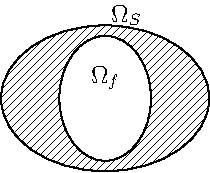
\includegraphics[width=0.3\textwidth]{Figs/domains}
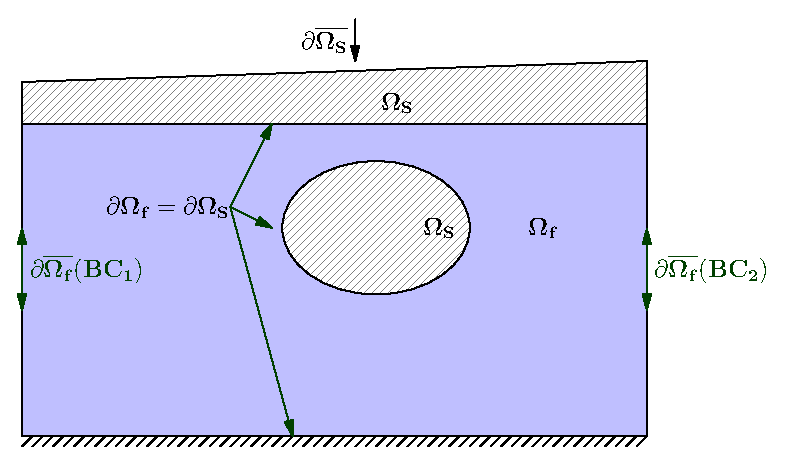
\includegraphics[width=0.8\textwidth]{Figs/walls}
\caption{Computational domain showing respective fluid
and solid subdomains, \(\Omega_f\) and \(\Omega_s\). The shared boundaries are denoted \(\partial\Omega_f=\partial\Omega_s\) and the solid boundary which is not shared by fluid is \(\overline{\partial\Omega_s}\), while the fluid boundary not shared by solid \(\overline{\partial\Omega_f}\).}
\label{fig:domains}
\end{figure}

\section{Incompressible Navier--Stokes equations}
%
The governing equations of flow motion in dimensional form are
\begin{eqnarray}\label{eq:ns_momentum}
\rho(\partial_{t} \mathbf u +\mathbf u \cdot \nabla \mathbf u) = - \nabla p + \nabla \cdot \tau + \rho {\bf f} \,\, , \text{in } \Omega_f , \quad \text{  (Momentum)  } 
\end{eqnarray}
where \( \tau=\mu[\nabla \vect u+\nabla \vect u^{T}]\).
\begin{eqnarray}\label{eq:ns_cont}
 \nabla \cdot \mathbf u =0 \,\, , \text{in } \Omega_f, \quad \text{  (Continuity)  }   
\end{eqnarray}

If the fluid viscosity is constant in the entire domain the viscous stress tensor can be contracted \(\nabla\cdot\tau=\mu\Delta \vect u\), therefore one may solve the Navier--Stokes equations in either the stress formulation, or no stress

\begin{itemize}
\item Variable viscosity requires the full stress tensor \(\nabla \cdot \tau=\nabla \cdot \mu[\nabla \vect u+\nabla \vect u^{T}]\), and we shall refer to this as the stress formulation
\item Constant viscosity leads to a simpler stress tensor \(\nabla \cdot \tau=\mu\Delta \vect u\), which we refer to as the 'no stress' formulation
\end{itemize}

\section{Non-dimensional Navier-Stokes}
Let us introduce the following non-dimensional variables \(\vect x^*\ = \frac{\vect x}{L}\), \(\vect u^*\ = \frac{u}{U}\), \(t^*\ = \frac{t}{L/U}\,\).
For the pressure scale we have two options 
\begin{itemize}
\item convective effects are dominant i.e. high velocity flows
\( p^* = \frac{p}{\rho U^2} \)
\item viscous effects are dominant i.e. creeping flows (Stokes flow)
\( p^* = \frac{p L}{\mu U} \)
\end{itemize}
For highly convective flows we choose the first scaling of the pressure and obtain the non-dimensional Navier-Stokes:
\begin{equation}\label{eq:NS_nondim}
\frac{\partial \mathbf{u^*}}{\partial t^*} + \mathbf{u^*} \cdot \nabla \mathbf{u^*}\ = -\nabla p^* + \frac{1}{Re} \nabla\cdot \tau^* + \frac{1}{Fr}\frac{\mathbf{f}}{g}.
\end{equation}
where \( \tau^*=[\nabla \vect u^*+\nabla \vect u^{*T}]\).
The two non-dimensional numbers here are the Reynolds number \(Re=\frac{\nu}{U L}\) \(Fr\) and the Froude number, defined as \(Fr = \frac{U^2}{gL}\).
%The above governing equations are subject to boundary conditions
%and initial conditions described in the following sections.
%
%\begin{tabular}{ l|l|l|l| }
%   \hline
%   Equation &  & &\\ \hline \hline
%   Incompressible NS (stress)& \ref{eq:ns_momentum} & \ref{eq:ns_cont}, \((4)=0\) & \\ 
%   Incompressible NS (non-stress)& \ref{eq:ns_momentum}, \((3)=\Delta \vect u\) & \ref{eq:ns_cont}, \((4)=0\) \\ 
%   Incompressible NS (non-stress)+Energy& \ref{eq:ns_momentum}, \((3)=\Delta \vect u\) & \ref{eq:ns_cont},\((4)=0\)& \ref{eq:energy} \\ 
%   Unsteady Stokes (non-stress)& \ref{eq:ns_momentum}, \((2)=0\( & \ref{eq:ns_cont},\((4)=0\)&  \\ 
%   Steady Stokes (non-stress)& \ref{eq:ns_momentum}, \((1)=0\), \((2)=0\) & \ref{eq:ns_cont},\((4)=0\)&  \\
%   Steady Heat transfer& --- & ---&  \ref{eq:energy}, \((5)=0\), \((6)=0\)\\
%   Compressible NS, Low Mach (non-stress)& \ref{eq:ns_momentum}, \((3)=\Delta \vect u\) & \ref{eq:ns_cont}, \((4)\neq 0\) \ref{eq:energy} + EOS &\ref{eq:energy} \\ 
%   \hline
%\end{tabular}

%\newline
\section{Energy equation}
In addition to the fluid flow, Nek5000 computes automatically the energy equation
\begin{eqnarray}\label{eq:energy}
 \rho c_{p} ( \partial_{t} T + \mathbf u \cdot \nabla T ) =
   \nabla \cdot (k \nabla T) + q_{vol}\,\, ,\text{in } \Omega_f\cup \Omega_s  \text{  (Energy)  } 
\end{eqnarray}

\section{Non-dimensional energy/passive scalar equation}
A similar non-dimensionalization as for the flow equations using the non-dimensional variables
\(\vect x^*\ = \frac{\vect x}{L}\),  \(\vect u^*\ = \frac{u}{U}\), \(t^*\ = \frac{t}{L/U}\), \(T=\frac{T^*-T_0}{\delta T}\) leads to
\begin{eqnarray}\label{eq:energy_nondim}
\partial_{t^*} T^* + \vect u^* \cdot \nabla T^* =
  \frac{1}{Pe} \nabla \cdot \nabla T^* + q_{vol}\,\, ,\text{in } \Omega_f\cup \Omega_s  \text{  (Energy)  } 
\end{eqnarray}
where \(Pe=LU/\alpha\), with \(\alpha=k/\rho c_p\).


\section{Passive scalars}\label{sec:passive_scal}

We can additionally solve a convection-diffusion equation for each passive scalar \(\phi_i\),
\(i\)=1,2,\(\ldots\) in \(\Omega_f \cup \Omega_s\)
\begin{eqnarray}\label{eq:pass_scal}
   (\rho c_{p})_i ( \partial_{t} \phi_{i} + \mathbf u \cdot \nabla \phi_{i} ) =
   \nabla \cdot (k_i \nabla \phi_{i}) + (q_{vol})_i.
\end{eqnarray}

The terminology and
restrictions of the temperature equations are retained for
the passive scalars, so that it is the responsibility of the
user to convert the notation of the passive scalar
parameters to their thermal analogues.
For example, in the context of mass transfer,
the user should recognize that the values specified
for temperature and heat flux
will represent concentration and mass flux, respectively.
Any combination of these equation characteristics is permissible with the
following restrictions. First, the equation must be set to unsteady if it is
time-dependent or if there is any type of advection. For these cases, the
steady-state (if it exists) is found as stable evolution of the
initial-value-problem. Secondly, the stress formulation must be selected if
the geometry is time-dependent. In addition, stress formulation must be
employed if there are traction boundary conditions applied on any fluid
boundary, or if any mixed velocity/traction boundaries, such as symmetry and
outflow/n, are not aligned with either one of the Cartesian \(x,y\) or \(z\) axes.
Other capabilities of Nek5000 are the linearized Navier-Stokes for flow stability, magnetohydrodynamic flows etc.



\section{Unsteady Stokes }
In the case of flows dominated by viscous effects Nek5000 can solve the reduced Stokes equations
\begin{eqnarray}\label{eq:ns_momentum_stokes}
 \rho(\partial_{t} \mathbf u ) = - \nabla p + \nabla \cdot \tau + \rho {\bf f} \,\, , \text{in } \Omega_f \text{  (Momentum)  }
\end{eqnarray}
where \(\nabla \cdot\tau=\nabla\cdot\mu[\nabla \vect u+\nabla \vect u^{T}]\) and
\begin{eqnarray}\label{eq:ns_cont_stokes}
 \nabla \cdot \mathbf u =0 \,\, , \text{in } \Omega_f  \text{  (Continuity)  } 
\end{eqnarray}
Also here we can distinguish between the stress and non-stress formulation according to whether the viscosity is variable or not. The non-dimensional form of these equations can be obtained using the viscous scaling of the pressure.


\section{Steady Stokes }
If there is no time-dependence, then Nek5000 can further reduce to
\begin{eqnarray}\label{eq:ns_momentum_steady_stokes}
 - \nabla p + \nabla \cdot \tau + \rho {\bf f}=0 \,\, , \text{in } \Omega_f \text{  (Momentum)  }
\end{eqnarray}
where \(\nabla \cdot\tau=\nabla\cdot\mu[\nabla \vect u+\nabla {\vect u}^{T}]\) and
\begin{eqnarray}\label{eq:ns_cont_steady_stokes}
 \nabla \cdot \mathbf u =0 \,\, , \text{in } \Omega_f  \text{  (Continuity)  } 
\end{eqnarray}

\section{Linearized Equations}
In addition to the basic evolution equations described above, Nek5000
provides support for the evolution of small perturbations about
a base state by solving the {\em linearized equations}
\begin{equation} \label{eq:pertu}
  \rho(\partial_{t} {\mathbf u_i}' + \mathbf u \cdot \nabla {\mathbf u_i}^{'} + \mathbf u_i' \cdot \nabla \mathbf u) =
   - \nabla p_i' + \mu \nabla^2 \mathbf u_i', \qquad \nabla \cdot \mathbf u_i' = 0,
\end{equation}
for multiple perturbation fields \(i=1,2,\dots\) subject to different initial
conditions and (typically) homogeneous boundary conditions.  
These solutions can be evolved concurrently with the base fields \((\mathbf u,p,T)\).
There is also
support for computing perturbation solutions to the Boussinesq equations for
natural convection.  Calculations such as these can be used to estimate Lyapunov exponents of chaotic flows, etc.



\section{Steady conduction}    
The energy Eq.~\ref{eq:energy} in which the advection term \(\mathbf u \cdot \nabla T\)
    and the transient term \(\partial_{t} T\) are zero. In essence this represents a Poisson equation.
    

\section{Low-Mach Navier-Stokes}\label{sec:lowma}
The compressible Navier-Stokes differ mathematically from the incompressible ones mainly in the divergence constraint \(\nabla \cdot \vect u\neq 0\). In this case the system of equations is not closed and an additional equation of state (EOS) is required to connect the state variables, e.g. \(p=f(\rho,T)\). However Nek5000 can only solve the Low Mach approximation of the compressible Navier-Stokes. The Low-Mach approximation decouples the pressure from the velocity leading to a system of equations which can be solved numerically in a similar fashion as the incompressible Navier-Stokes.

The Low Mach equations in non-dimensional form are 
\begin{eqnarray}
&&\rho\bigg(\frac{\d \vect u}{\d t}+ \vect u\cdot\nabla\vect u\bigg)=-\nabla p+\nabla \cdot\bb\tau+\rho\vect f\ \\ \nonumber
&&\frac{\d \vect \rho}{\d t}+ \vect u\cdot\nabla\vect \rho=-\rho\nabla \cdot \vect u\\ \nonumber
&&\rho\bigg(\frac{\d T}{\d t}+ \vect u\cdot\nabla T\bigg)=-\nabla \cdot k \nabla T\\ \nonumber
\end{eqnarray}
where \(\bb\tau=\mu[\nabla \vect u+\nabla \vect u^{T}-\frac{2}{3}\nabla \cdot \vect u \vect I]\).


The implementation of the equation if state for the Low Mach formulation is for the moment hard-coded to be the ideal gas equation of state \(p=\rho R T\). This allows for both variable density and variable viscosity. The system is solved by substituting \(\rho=f(p,T)\) into the continuity equation and obtaining a so-called thermal divergence (the term \(\nabla \cdot \mathbf u\) is given as a function of the temperature).
A more detailed description on how these equations connect is given in section \ref{sec:lowma} as well as in the developer's manual.

\section{Incompressible MHD equations}\label{sec:mhd}
Magnetohydrodynamics is based on the idea that magnetic fields can induce currents in a moving conductive fluid, which in turn creates forces on the fluid and changing the magnetic field itself. The set of equations which describe MHD are a combination of the Navier-Stokes equations of fluid dynamics and Maxwell's equations of electromagnetism. These differential equations have to be solved simultaneously, and Nek5000 has an implementation for the incompressible MHD.

Consider a fluid of velocity \(\vect u\) subject to a magnetic field \(\vect B\) then the incompressible MHD equations are
\begin{eqnarray}
 \rho(\partial_{t} \mathbf u + \mathbf u \cdot \nabla \mathbf u) &=& - \nabla p + \mu \Delta \mathbf u + \bB\cdot \nabla \bB \ ,\\ 
 \nabla \cdot \mathbf u & =& 0\\ \nonumber
   \partial_{t} \bB + \mathbf u \cdot \nabla \bB &=& - \nabla q + \eta \Delta \bB + \bB\cdot \nabla \mathbf u \ ,\\ 
    \nabla \cdot \bB & =& 0 \nonumber
\end{eqnarray}
where \(\rho\) is the density \(\mu\) the viscosity, \(\eta\) resistivity, and pressure \(p\).


The total magnetic field can be split into two parts: \( \mathbf{B} = \mathbf{B_0} + \mathbf{b} \) (mean + fluctuations). The above equations become in terms of Els\"asser variables (\(\mathbf{z}^{\pm} =  \mathbf{u} \pm \mathbf{b} \)) 
\begin{eqnarray}
\frac{\partial {\mathbf{z}^{\pm}}}{\partial t}\mp\left(\mathbf {B}_0\cdot{\mathbf \nabla}\right){\mathbf z^{\pm}} + \left({\mathbf z^{\mp}}\cdot{\mathbf \nabla}\right){\mathbf z^{\pm}} = -{\mathbf \nabla}p 
+ \nu_+ \nabla^2 \mathbf{z}^{\pm} + \nu_- \nabla^2 \mathbf{z}^{\mp} 
\end{eqnarray}
where \( \nu_\pm = \nu \pm \eta \).

The important non-dimensional parameters for MHD are \(Re = U L /\nu \) and the magnetic Re \( Re_M = U L /\eta \).


\subsection{Adaptive Lagrangian-Eulerian (ALE)}

We consider unsteady incompressible flow in a domain with moving boundaries:
\begin{eqnarray} \label{eq:mhd1}
\frac{\partial\mathbf u}{\partial t}&=&-\nabla p +\frac{1}{Re}\nabla\cdot(\nabla + \nabla^T)\mathbf u  + NL,\\
 \nabla \cdot \mathbf u &= &0 
\end{eqnarray}
Here, \(NL\) represents the quadratic nonlinearities from the convective term.

Our free-surface hydrodynamic formulation is based upon the arbitrary 
Lagrangian-Eulerian (ALE) formulation described in \cite{ho89}.
Here, the domain \(\Omega(t)\) is also an unknown.  As with the velocity,
the geometry \(\vect x\) is represented by high-order polynomials.
For viscous free-surface flows,
the rapid convergence of the high-order surface approximation to the 
physically smooth solution minimizes surface-tension-induced stresses
arising from non-physical cusps at the element interfaces, 
where only \(C^0\) continuity is enforced.  
The geometric deformation is specified by a mesh velocity \(\vect w := \dot{\vect x}\)
that is essentially arbitrary, provided that \(\vect w\) satisfies the kinematic
condition \(\vect w \cdot \hat{\vect n}|^{}_{\Gamma} = \vect u \cdot \hat{\vect n}|^{}_{\Gamma}\),
where \(\hat{\vect n}\) is the unit normal at the free surface \(\Gamma(x,y,t)\).
The ALE formulation provides a very accurate description of the free
surface and is appropriate in situations where wave-breaking does not occur.

To highlight the key aspects of the ALE formulation, we introduce
the weighted residual formulation of (\ref{eq:mhd1}):
{\em Find \((\bu,p) \in X^N \times Y^N\) such that:}
\begin{eqnarray} \label{eq:wrt1}
\dd{}{t} (\vect v,\vect u) = (\nabla \cdot \vect v,p) - \frac{2}{Re}(\nabla \vect v,\vect S)
+(\vect v,N\!L) + c(\vect v,\vect w,\vect u),
\qquad
(\nabla \cdot \vect u,q) = 0,
\end{eqnarray} 
for all test functions \((\vect v,q) \in X^N \times Y^N\).
Here \((X^N,Y^N)\) are the compatible velocity-pressure approximation 
spaces introduced in \cite{mapa89}, 
\((.,.)\) denotes the inner-product
\((\vect f,\vect g) := \int_{\Omega(t)} \vect f \cdot \vect g \,dV\),
and 
\(\vect S\) is the stress tensor 
\(S_{ij}^{} := \frac{1}{2}( \pp{u_i}{x_j} + \pp{u_j}{x_i} )\).
For simplicity, we have neglected the surface tension term.
A new term in (\ref{eq:wrt1}) is the trilinear form
involving the mesh velocity
\begin{eqnarray} \label{eq:trilin}
c(\vect v,\vect w,\vect u) :=
\int_{\Omega(t)}^{}
\sum_{i=1}^3 
\sum_{j=1}^3 v_i^{} \pp{w_j^{} u_i^{}}{x_j^{}} \,dV,
\end{eqnarray} 
which derives from the Reynolds transport theorem when
the time derivative is moved outside the bilinear form \((\vect v,\vect u_t^{})\).
The advantage of (\ref{eq:wrt1}) is that it greatly simplifies the
time differencing and avoids grid-to-grid interpolation as the domain
evolves in time.  With the time derivative outside of the integral, 
each bilinear or trilinear form involves functions at a specific time,
\(t^{n-q}\), integrated over \(\Omega(t^{n-q})\).
For example, with a second-order backward-difference/extrapolation scheme,
the discrete form of (\ref{eq:wrt1}) is
\begin{eqnarray} \label{eq:bdk}
\frac{1}{2 \dt}\left[ 
 3 (\vect v^n,\vect u^n)^n
-4 (\vect v^{n-1},\vect u^{n-1})^{n-1}
 + (\vect v^{n-2},\vect u^{n-2})^{n-2} \right]
= L^n (\vect u) + 
2 \widetilde{N\!L}^{n-1}
- \widetilde{N\!L}^{n-2}.
\end{eqnarray} 
Here, \(L^n(\vect u)\) accounts for all {\em linear} terms in (\ref{eq:wrt1}),
including the pressure and divergence-free constraint, which are evaluated
implicitly (i.e., at time level \(t^n\), on \(\Omega(t^n)\)), and
\(\widetilde{N\!L}^{n-q}\) accounts for all {\em nonlinear} terms, including
the mesh motion term (\ref{eq:trilin}), at time-level \(t^{n-q}\).
The superscript on the inner-products \((.,.)^{n-q}\) indicates 
integration over \(\Omega(t^{n-q})\). 
The overall time advancement is as follows.  
The mesh position \(\vect x^n \in \Omega(t^n)\) is computed
explicitly using \(\vect w^{n-1}\) and \(\vect w^{n-2}\);
the new mass, stiffness, and gradient operators involving integrals
and derivatives on \(\Omega(t^n)\) are computed;  
the extrapolated right-hand-side terms are evaluated; and 
the implicit linear system is solved for \(\vect u^n\).   
Note that it is only the {\em operators} that are updated,
not the {\em matrices}.  Matrices are never formed in Nek5000 and
because of this, the overhead for the moving domain formulation
is very low.


%\section{Nek5000 code layout}
%\input{code_layout}

\chapter{Quick start}
\section{Download and Build}
This chapter provides a quick overview to using Nek5000
for some basic flow problems provided in the {\tt .../examples}
directory.
           
Nek5000 runs under Linux or any Linux-like OS such as MAC, AIX, BG, Cray etc.
The source is maintained in a legacy SVN repository (last updated June 2, 2016)
and up-to-date Git repositories.  Both repositories are available for
download, but we recommended that new users work with the Git repositories.  

\section{The Git Repositories}

\subsection{Downloading the source code}
The Nek5000 source code is hosted on GitHub at \url{https://github.com/Nek5000/Nek5000}.  You can download the source code as a .zip file\footnote{https://github.com/Nek5000/Nek5000/archive/master.zip} or a .tar.gz archive\footnote{https://github.com/Nek5000/Nek5000/archive/master.tar.gz}.  You can also download (or ``clone'') the repository itself.  The following commands will clone the repository in a directory named {\tt \$HOME/Nek5000} (where {\tt \$HOME} denotes your home directory):
\begin{verbatim}
cd && git clone https://github.com/Nek5000/Nek5000.git -b master
\end{verbatim}
You can also clone the repository in any directory of your choice:
\begin{verbatim}
cd $HOME/my-repos/ && git clone https://github.com/Nek5000/Nek5000.git -b master
\end{verbatim}

\subsection{Downloading the example problems}
The Nek5000 example problems are hosted in a second repository on GitHub, \url{https://github.com/Nek5000/NekExamples}.  Likewise, you can download the examples as a .zip archive\footnote{https://github.com/Nek5000/NekExample/archive/master.zip}, a .tar.gz archive\footnote{https://github.com/Nek5000/NekExamples/archive/master.tar.gz}, or you may clone the repository to your home directory:
\begin{verbatim}
cd && git clone https://github.com/Nek5000/NekExamples.git -b master
\end{verbatim}
or a directory of your choice:
\begin{verbatim}
cd $HOME/my-repos/ && git clone https://github.com/Nek5000/Nek5000.git -b master
\end{verbatim}

\subsection{Tools and scripts}

The {\tt Nek5000/tools} directory contains programs for pre- and
post-processing tasks, such as generating meshes from geometry descriptions.  The following commands will build the tools in {\tt \$HOME/bin}:
\begin{verbatim}
cd Nek5000/tools && ./maketools all
\end{verbatim}
By default, the {\tt maketools} script will use gfortran and gcc as the
Fortran and C compilers; you can specify a different set of compilers by
editing {\tt maketools}.  You can also build the tools in another
directory of your choice by providing a second argument to {\tt maketools}; for example:
\begin{verbatim}
cd $HOME/my-repos/Nek5000/tools && ./maketools all $HOME/my-tools-bin/
\end{verbatim}

Besides the compiled tools, there are several convenience scripts in {\tt
Nek5000/bin} that allow you to easily set up and execute runs of Nek5000.
These scripts are executable as-is and do not need to be compiled. 

We recommend that you add the paths to the tools and scripts to the {\tt \$PATH}
variable in your shell's environment.  This will allow you execute the tools
and scripts without typing the full path to the executables.  In the bash
shell, if you have cloned Nek5000 in {\tt \$HOME/Nek5000} and compiled tools in
{\tt \$HOME/bin}, you can edit your executable path with:
\begin{verbatim}
export PATH="$HOME/bin:$HOME/Nek5000/bin:$PATH"
\end{verbatim}
or if the Nek5000 repository and tools are in custom locations, use:
\begin{verbatim}
export PATH="$HOME/my-tools-bin:$HOME/my-repos/Nek5000/bin:$PATH"
\end{verbatim}
In the following examples, we will assume that the tools and scripts have been
added to your {\tt \$PATH}.

\section{The SVN Repository}

\subsection{Downloading the source code and examples}

The SVN repository can be downloaded with the following commands:
\begin{verbatim}
cd && svn co https://svn.mcs.anl.gov/repos/nek5 nek5_svn
\end{verbatim}
This will create a directoy named {\tt nek5\_svn} in your home directory.  The
example problems are included in the same SVN repo and do not need to be downloaded separately.

\subsection{Tools and scripts}
The {\tt nek5\_svn/trunk/tools} directory contains programs for pre- and
post-processing tasks, such as generating meshes from geometry descriptions.  The following commands will build the tools in {\tt \$HOME/bin}:
\begin{verbatim}
cd $HOME/nek5_svn/trunk/tools && ./maketools all
\end{verbatim}
By default, the {\tt maketools} script will use gfortran and gcc as the
Fortran and C compilers; you can specify a different set of compilers by
editing {\tt maketools}.  
%\footnote{In some cases it may be necessary to reduce the memory
%footprint of some of the tools. The procedures are (will be)
%described in \sc{sec. troubleshooting}.}

Besides the compiled tools, there are several convenience scripts in {\tt
nek5\_svn/trunk/tools/scripts} that allow you to easily set up and execute runs
of Nek5000.  These scripts are executable as-is and do not need to be compiled. 

We recommend that you append the paths to the tools and scripts to the {\tt \$PATH}
variable in your shell's environment.  This will allow you execute the tools
and scripts without typing the full path to the executables.  In the bash
shell, you can edit your executable path with:
\begin{verbatim}
export PATH="$HOME/bin:$HOME/nek5_svn/trunk/tools/scripts:$PATH"
\end{verbatim}
In the following examples, we will assume that the tools and scripts have been
added to your {\tt \$PATH}.

\section{A worked example}
\section{A Worked Example}
As a first example, we consider the eddy problem due to Walsh 
\footnote{O. Walsh, ``Eddy solutions of the Navier-Stokes equations,''
{\em The NSE II-Theory and Numerical Methods}, J.G. Heywood, K. Masuda, 
R. Rautmann, and V.A. Solonikkov, eds., Springer, pp.  306--309 (1992)}.
To get started, execute the following commands for the Git repositories:
\begin{verbatim}
cd
mkdir eddy
cd eddy
cp $HOME/NekExamples/eddy/* .
cp $HOME/Nek5000/core/makenek .
\end{verbatim}
or the equivalent commands for the SVN repository:
\begin{verbatim}
cd
mkdir eddy
cd eddy
cp $HOME/nek5_svn/examples/eddy/* .
cp $HOME/nek5_svn/trunk/nek/makenek .
\end{verbatim}

{\bf Modify {\tt makenek}.}

If you do not have {\tt mpi} installed on your system, edit {\tt makenek},
uncomment the {\tt IFMPI="false"} flag, and change the Fortran and C
compilers according to what is available on your machine.  (Most any
Fortran compiler save g77 or g95 will work.)

Nek5000 is written in F77 which has implicit typesetting as default. This means in practice that if the user defines a new variable in the user file and forgets to define its type explicitly then variable beginning with a character from I to N, its type is {\tt INTEGER}. Otherwise, it is {\tt REAL}. 

This common type of mistake for a beginner can be avoided using a warning flag {\tt -Wimplicit}. This flag warns whenever a variable, array, or function is implicitly declared. Has an effect similar to using the IMPLICIT NONE statement in every program unit. 

Another useful flag may {\tt -mcmodel} which allows for arrays of size larger than 2GB. This option tells the compiler to use a specific memory model to generate code and store data. It can affect code size and performance. If your program has global and static data with a total size smaller than 2GB, {\tt -mcmodel=small} is sufficient. Global and static data larger than 2GB requires {\tt -mcmodel=medium} or {\tt -mcmodel=large}.


If you have {\tt mpi} installed on your system or have made the prescribed
changes to makenek, the eddy problem can be compiled as follows


{\bf Compiling nek.}
{\tt makenek eddy\_uv} 

\noindent
If all works properly, upon comilation the executable {\tt nek5000} will be generated using {\tt eddy\_uv.usr} to provide
user-supplied initial conditions and analysis.  Note that if you encountered
a problem during a prior attempt to build the code you should type

{\tt makenek clean;}  

{\tt makenek eddy\_uv} 

\noindent
Once compilation is successful, start the simulation by typing
 

{\bf Running a case:}
{\tt nekb eddy\_uv } 

which runs the executable in the background ({\tt nekb}, as opposed to {\tt
nek}, which will run in the foreground).  
If you are running on a multi-processor machine that supports MPI, you
can also run this case via

{\bf A parallel run:}
{\tt nekbmpi eddy\_uv 4}

\noindent
which would run on 4 processors.    If you are running on a system
that supports queuing for batch jobs (e.g., pbs), then the following
would be a typical job submission command

%% \marginlabel{\bf Running with pbs:}
{\tt nekpbs eddy\_uv 4}

In most cases, however, the details of the nekpbs script would need
to be modified to accommodate an individual's user account, the 
desired runtime and perhaps the particular queue.   Note that the
scripts {\tt nek, nekb, nekmpi, nekbmpi,} etc. perform some essential
file manipulations prior to executing {\tt nek5000}, so it is important
to use them rather than invoking {\tt nek5000} directly.


To check the error for this case, type
\begin{verbatim}
grep -i err eddy_uv.log | tail
\end{verbatim}
or equivalently
\begin{verbatim}
grep -i err logfile | tail
\end{verbatim}
where, because of the {\tt nekb} script, {\tt logfile} is 
linked to the {\tt .log} file of the given simulation. 
If the run has completed, the above {\tt grep} command should yield lines like
\scriptsize
\begin{verbatim}
 1000  1.000000E-01  6.759103E-05  2.764445E+00  2.764444E+00  1.000000E+00  X err
 1000  1.000000E-01  7.842019E-05  1.818632E+00  1.818628E+00  3.000000E-01  Y err
\end{verbatim}
\normalsize
which gives for the $x$- and $y$-velocity components the 
step number, the physical time, the maxiumum error, the maximum exact
and computed values and the mean (bulk) values.

A common command to check on the progress of a simulation is
\begin{verbatim}
grep tep logfile | tail
\end{verbatim}
which typically produces lines such as
\scriptsize
\begin{verbatim}
Step    996, t= 9.9600000E-02, DT= 1.0000000E-04, C=  0.015 4.6555E+01 3.7611E-02
\end{verbatim}
\normalsize
indicating, respectively, the step number, the physical time, the
timestep size, the Courant (or CFL) number, the cumulative wall clock time (in seconds)
and the wall-clock time for the most recent step.   Generally, one would 
adjust $\dt$ to have a CFL of $\sim$0.5.  


%See Section \ref{sec:timestepping} for a comprehensive discussion of timestep selection.

\section{Viewing the First 2D Example}

The preferred mode for data visualization and analysis with Nek5000 is
to use VisIt.  For a quick
peek at the data, however, we list a few commands for the native Nek5000 
postprocessor.   Assuming that the {\tt maketools} script has been executed
and that {\tt /bin} is in the execution path, then typing 

\noindent
{\tt postx} 

\noindent
in the working directory should open a new window with a sidebar menu.
With the cursor focus in this window (move the cursor to the window and
left click), hit {\tt return} on the keyboard accept the default session name and click {\sc plot} with the left mouse button.  This should bring up
a color plot of the pressure distribution for the first output file
from the simulation (here, {\tt eddy\_uv.fld01}), which contains the
geometry, velocity, and pressure.  

Alternatively one can use the script \textit{visnek}, to be found in {\tt /scripts}. It is sufficent to run 

\noindent
{\tt visnek eddy\_uv}\textit{ (or the name of your session)}

to obatain a file named {\tt eddy\_uv.nek5000} which can be recognized in VisIt \footnote{https://wci.llnl.gov/simulation/computer-codes/visit/}


\begin{comment}
To see the vorticity at the final time, load the last output file,
{\tt eddy\_uv.fld12}, by clicking/typing the following in the postx window:
\begin{tabular}{r l l l}
  & {\bf click} \hspace*{1in} &{\bf type} \hspace*{1in} & {\bf comment} \\ \hline
1.& SET TIME         & 12 & load fld12 \\
2.& SET QUANTITY \\
3.& VORTICITY \\
4.& PLOT 
\end{tabular}
\end{comment}

{\bf Plotting the error:}
For this case, the error has been written to {\tt
eddy\_uv.fld11} by making a call to {\tt outpost()} in the {\tt userchk()}
routine in {\tt eddy\_uv.usr}.  The error in the velocity components
is stored in the velocity-field locations and can be viewed with 
postx, or VisIt as before.

\begin{comment}
through the following sequence: 
\begin{tabular}{r l l l}
  & {\bf click} \hspace*{1in} &{\bf type} \hspace*{1in} & {\bf comment} \\ \hline
1.& SET TIME         & 11 & load fld11 \\
2.& SET QUANTITY \\
3.& VELOCITY \\
4.& MAGNITUDE \\
5.& PLOT  \\
\end{tabular}
\end{comment}

\subsection{Modifying the First Example}

A common step in the Nek5000 workflow is to rerun with a higher
polynomial order.   Typically, one runs a relatively low-order case
(e.g., {\tt lx1}=5) for one or two flow-through times and then uses
the result as an initial condition for a higher-order run
(e.g., {\tt lx1}=8).  We illustrate the procedure with the 
{\tt eddy\_uv} example.

Assuming that the contents of {\tt nek5\_svn/trunk/tools/scripts}
are in the execution path, begin by typing
\begin{verbatim}
cp eddy_uv eddy_new
\end{verbatim}
which will copy the requisite {\tt eddy\_uv} case files
to {\tt eddy\_new}.  
Next, edit {\tt SIZE} and change the two lines defining
{\tt lx1} and {\tt lxd} from
\begin{verbatim}
      parameter (lx1=8,ly1=lx1,lz1=1,lelt=300,lelv=lelt)
      parameter (lxd=12,lyd=lxd,lzd=1)
\end{verbatim}
to
\begin{verbatim}
      parameter (lx1=12,ly1=lx1,lz1=1,lelt=300,lelv=lelt)
      parameter (lxd=18,lyd=lxd,lzd=1)
\end{verbatim}
Then recompile the source by typing
\begin{verbatim}
makenek eddy_new
\end{verbatim}

Next, edit {\tt eddy\_new.rea} and change the line 
\begin{verbatim}
            0 PRESOLVE/RESTART OPTIONS  *****
\end{verbatim}
(found roughly 33 lines from the bottom of the file) to
\begin{verbatim}
            1 PRESOLVE/RESTART OPTIONS  *****
eddy_uv.fld12
\end{verbatim}
which tells nek5000 to use the contents of {\tt eddy\_uv.fld12}
as the initial condition for {\tt eddy\_new}.
The simulation is started in the usual way:
\begin{verbatim}
nekb eddy_new
\end{verbatim}
after which the command
\begin{verbatim}
grep err logfile | tail
\end{verbatim}
will show a much smaller error ($\sim 10^{-9}$) than the {\tt lx1=8}
case. 

Note that one normally would not use a restart file for the {\em eddy}
problem, which is really designed as a convergence study.  The purpose here, however, was two-fold, namely,
to illustrate a change of order and its impact on the error, and to
demonstrate the frequently-used restart procedure. However for a higher order timestepping scheme an accurate restart would require a number of field files of the same size (+1) as the order of the multistep scheme


\chapter{User files}
\section{Case set-up .usr}

%Nek5000 consists of three principal modules:  the preprocessor
%{\tt prex}, the solver {\tt nek5000}, and the postprocessor {\tt postx}.
%{\tt prex} and {\tt postx} are based upon an X-windows GUI.  

Each simulation is defined by three files, the .rea file, the .usr file,
and the SIZE file.  In addition, there is a derived .map file that is
generated from the .rea file by running {\tt genmap} which will determine how the elements will be split across processors in the case of a parallel run.
%Suppose you are doing a calculation called ``shear.''
%The key files defining the problem would be shear.rea, shear.map, and shear.usr.
SIZE controls (at compile time) the polynomial degree used in the simulation,
as well as the space dimension $d=2$ or 3.

The SESSION.NAME file contains the current run, it must provide the name of the .rea file and the path to it.  It does not however need to correspond to an .usr file of an identical name. This allows for different test cases (.usr files) that use the same geometry and boundary conditions (.rea files).

This chapter provides an introduction to the basic files required
to set up a Nek5000 simulation.

%\marginlabel{\bf {\tt .usr} files:}
\subsection{Contents of .usr file}

The most important interface to Nek5000 is the
set of Fortran subroutines that are contained in the {\tt .usr} file.
This file allows direct access to all runtime variables.
Here, the user may specify spatially varying properties
(e.g., viscosity), volumetric heating sources, body forces, and so forth.
One can also specify arbitrary initial and boundary conditions through
the routines {\tt useric()} and {\tt userbc()}.
The routine {\tt userchk()} allows the user to interrogate the solution
at the end of each timestep for diagnostic purposes.   The {\tt .usr}
files provided in the {\tt /examples/... } directories illustrate
several of the more common analysis tools.  For instance, there are utilities
for computing the time average of $u$, $u^2$, etc. so that one can
analyze mean and rms distributions with the postprocessor.  There are
routines for computing the vorticity or the scalar $\lambda_2$ 
for vortex identification, and so forth.


\subsubsection*{Routines in .usr file}

The routine {\tt uservp} specifies the variable properties of the governing equations.
This routine is called once per processor, and once per discrete point therein. 
%For each field (fluid {\tt ifield.eq.1}, passive scalar {ifield.eq.2}(3,4..)) we have to specify two %components, {\tt utrans} corresponding to the transport term ($\rho$ in Eq.\ref{eq:ns_momentum}, $\rhocp$ in %Eq
\\

\begin{tabular}{ l|l|l|l }
   \hline
   Equation & {\tt udiff} & {\tt utrans} & {\tt ifield} \\ \hline \hline
   Momentum Eq.\ref{eq:ns_momentum} & $\rho$ & $\mu$ & 1 \\ 
   Energy Eq.\ref{eq:energy} & $\rho c_p$ & $k$ & 2\\ 
   Passive scalar Eq.\ref{eq:pass_scal} &$(\rho c_p)_i$ & $k_i$& i-1\\
   \hline
\end{tabular}


\begin{lstlisting}
      subroutine uservp (ix,iy,iz,eg)
      include 'SIZE'
      include 'TOTAL'
      include 'NEKUSE'
      
      integer iel
      iel = gllel(eg)

      udiff =0.
      utrans=0.
      
      return
      end
\end{lstlisting}

The routine {\tt userdat} is called right after the geometry is loaded into NEK5000 and prior to the distribution of the GLL points. This routine is called once per processor but for all the data on that processor. At this stage the elements can be modified as long as the topology is preserved. It is also possible to alter the type of boundary condition that is initially attributed in the {\tt .rea} file, as illustrated below (the array {\tt cbc(face,iel,field}) contains the boundary conditions per face and field of each element). Note the spacing allocated to each BC string is of three units.

\begin{lstlisting}
      subroutine usrdat
      include 'SIZE'
      include 'TOTAL'
      include 'NEKUSE'
      integer iel,f

      do iel=1,nelt  !  Force flux BCs
      do f=1,2*ndim
         if (cbc(f,iel,1).eq.'W  ') cbc(f,iel,2) = 'f  ' ! flux BC for temperature
      enddo
      enddo
   
      return
      end
\end{lstlisting}

The routine {\tt usrdat2} is called after the GLL points were distributed and allows at this point only for affine transformations of the geometry.
\begin{lstlisting}
      subroutine usrdat2
      include 'SIZE'
      include 'TOTAL'

      return
      end
\end{lstlisting}

The routine {\tt userf} is called once for each point and provides the force term in Eq.\ref{eq:momentum}. Not that according to the dimensionalization in Eq.\ref{eq:momentum} the force term $\vect f$ is in fact multiplied by the density $\rho$.
\begin{lstlisting}
      subroutine userf  (ix,iy,iz,eg)
      include 'SIZE'
      include 'TOTAL'
      include 'NEKUSE'

      ffx = 0.0
      ffy = 0.0
      ffz = 0.0

      return
      end
\end{lstlisting}

Similarly to {\tt userf} the routine {\tt userq} provides the force term in Eq.\ref{eq:energy} and the subsequent passive scalar equations according to Eq.\ref{eq:pass_scal}.
\begin{lstlisting}	
      subroutine userq  (ix,iy,iz,eg)
      include 'SIZE'
      include 'TOTAL'
      include 'NEKUSE'
      
      qvol   = 0.

      return
      end
      \end{lstlisting}
      
      The boundary conditions are assigned in {\tt userbc} for both the fluid, temperature and all other scalars. An extensive list of such possible boundary conditions is available in Section.~\ref{sec:boundary}. 
      \begin{lstlisting}
      subroutine userbc (ix,iy,iz,iside,ieg)
      include 'SIZE'
      include 'TOTAL'
      include 'NEKUSE'

      ux=0.0
      uy=0.0
      uz=0.0
      temp=0.0
      flux = 1.0
      
      return
      end
\end{lstlisting}

Initial conditions are attributed in {\tt useric} similarly to the boundary conditions
\begin{lstlisting}
      subroutine useric (ix,iy,iz,ieg)
      include 'SIZE'
      include 'TOTAL'
      include 'NEKUSE'
   
      uy=0.0
      ux=0.0
      uz=1.0

      return
      end
      
\end{lstlisting}
The routine {\tt userchk} is called once per processor after each timestep (and once after the initialization is finished). This is the section where the solution can be interrogated and subsequent changes can be made.
\begin{lstlisting}
      subroutine userchk
      include 'SIZE'
      include 'TOTAL'
      include 'NEKUSE'

      call outpost(vx,vy,vz,pr,t,'ext')
           
      return
      end
      \end{lstlisting}
      
The routine {\tt usrdat3} is not widely used, however it shares the same properties with {\tt usrdat2}.
\begin{lstlisting}
      subroutine usrdat3
      include 'SIZE'
      include 'TOTAL'
c
      return
      end
\end{lstlisting}

Nek5000 can solve the dimensional or non-dimensional equations by setting the following parameters

\begin{table}

\begin{tabular}{ l|l| }
   \hline
   Dimensional parameters & Non-dimensional parameters\\ \hline \hline
{\tt p1}=$\rho$      &      {\tt p1}=1\\
{\tt p2}=$\nu$       &      {\tt p2}=1/Re (-Re)\\
{\tt p7}=$\rho C_p$  &      {\tt p7}=1\\
{\tt p8}=$k$         &      {\tt p8}=1/Pe (-Pe)\\
   \hline
\end{tabular}
\end{table}

alternatively the variable properties can be set in the USERVP routine.

 
\textbf{What is a SESSION file?}

To run NEK5000, each simulation must have a SESSION.NAME file. This file is read in by the code and gives the path to the relevant files describing the structure and parameters of the simulation. The SESSION.NAME file is a file that contains the name of the simulation and the full path to supporting files. For example, to run the eddy example from the repository, the SESSION.NAME file would look like:

\begin{verbatim}
eddy_uv\\
/homes/user\_ name/nek5\_ svn/examples/eddy/ 
\end{verbatim}


\section{Problem size file SIZE}
The SIZE file defines the problem size, i.e. spatial points at which the solution is to be evaluated within each element, number of elements per processor etc.
The SIZE file governs the memory allocation for most of the arrays
in Nek5000, with the exception of those required by the C utilities.
The primary parameters of interest in SIZE are: 
\begin{description}
\item{\bf ldim} = 2 or 3.  This must be set to 2 for
two-dimensional or axisymmetric simulations  (the latter
only partially supported) or to 3 for three-dimensional simulations.
\item{\bf lx1} controls the polynomial order of the approximation,
\(N\)={\tt lx1-1}.
\item{\bf lxd} controls the polynomial order of the integration for
convective terms.  Generally, {\tt lxd=3 * lx1/2}.  On some platforms, however,
it is important for memory access performance that {\tt lx1} and {\tt lxd} be even.
\item{\bf lx2} = {\tt lx1} or {\tt lx1-2}.  This determines the formulation for
the Navier-Stokes\index{Navier-Stokes} solver (i.e., the choice between the \(\PP_N\)--\(\PP_N\) 
or \(\PP_N\)--\(\PP_{N-2}\) methods) and the approximation order for the
pressure, {\tt lx2-1}.
\item{\bf lelt} determines the {\em maximum} number of elements 
{\em per processor}.
\end{description}

The total size of the problem is {\tt lx1*ly1*lz1*lelt}.

\subsection{Memory Requirements}

Per-processor memory requirements for  Nek5000 scale
roughly as 400 8-byte words per allocated gridpoint.  The number
of {\em allocated} gridpoints per processor is 
\(n_{\max}\)={\tt lx1*ly1*lz1*lelt}.  
(For 3D, {\tt lz1=ly1=lx1}; for 2D, {\tt lz1=1}, {\tt ly1=lx1}.)  
If required for a particular simulation, more memory may be made
available by using additional processors.  For example, suppose
one needed to run a simulation with 6000 elements of order \(N=9\).
To leading order, the total memory requirements would be
{\tt \(\approx E(N+1)^3\) points \(\times\) 400 (wds/pt) \(\times\) 8 bytes/wd =
6000 \(\times 10^3 \times 400 \times 8 \)= 19.2} GB.  Assuming there
is 400 MB of memory per core available to the user (after accounting
for OS requirements), then one could run this simulation with
{\tt \(P \ge 19,200\) \mbox{MB} \(/( 400 \)\mbox{MB/proc}) \(= 48\)} processors.
To do so, it would be necessary to set {\tt lelt} \(\ge\) 6000/48 = 125.

We note two other parameters of interest in the parallel context:
\begin{description}
\item{\bf lp}, the maximum number of processors that can be used.
\item{\bf lelg}, an upper bound on the number of elements in the simulation.
\end{description}
\noindent
There is a slight memory penalty associated with these variables, so
one generally does not want to have them excessively large.  It is 
common, however, to have lp be as large as anticipated for a given
case so that the executable can be run without recompiling on
any admissible number of processors (\(P_{\mbox{mem}} \le P \le E\),
where \(P_{\mbox{mem}}\) is the value computed above).


\section{Geometry and Parameters file .rea}


%\marginlabel{\bf {\tt .rea} files:}
The {\tt .rea} file consists of several sections:
\subsubsection*{ Parameters and logical switches}
\begin{description}
\item{\bf parameters} These control the runtime parameters such as viscosity,
    conductivity, number of steps, timestep size, order of the timestepping,
    frequency of output, iteration tolerances, flow rate, filter strength,
    etc.   There are also a number of free parameters that the user can
    use as handles to be passed into the user defined routines in the .usr file.
\item{\bf passive scalar data} This information can be specified also in the \texttt{.uservp} routine in the .usr file. If specified in the .rea file then the coefficients for the conductivity term are listed in ascending order for passive scalars ranging \texttt{1..9} followed by the values for the \(\rho c_p\) coefficients.
\begin{verbatim}
4  Lines of passive scalar data follows 2 CONDUCT; 2 RHOCP
   1.00000       1.00000       1.00000       1.00000       1.00000
   1.00000       1.00000       1.00000       1.00000
   1.00000       1.00000       1.00000       1.00000       1.00000
   1.00000       1.00000       1.00000       1.00000
\end{verbatim}
\item{\bf logicals} These determine whether one is computing a steady or unsteady
  solution, whether advection is turned on, etc.
\end{description}
\begin{comment}
           13  LOGICAL SWITCHES FOLLOW
  T     IFFLOW
  T     IFHEAT
  T     IFTRAN
  T T F F F F F F F F F IFNAV & IFADVC (convection in P.S. fields)
  F F T T T T T T T T T T IFTMSH (IF mesh for this field is T mesh)
  F     IFAXIS
  F     IFSTRS
  F     IFSPLIT
  F     IFMGRID
  F     IFMODEL
  F     IFKEPS
  F     IFMVBD
  F     IFCHAR
\end{comment}
\subsubsection*{Mesh and boundary condition info} 
\begin{description}
\item{\bf geometry} The geometry is specified in an arcane format specifying
    the \(xyz\) locations of each of the eight points for each element,
    or the \(xy\) locations of each of the four points for each element in 2D.
A line of the following type may be encountered at the beginning of the mesh section of the area file.    
\begin{verbatim}
3.33333       3.33333     -0.833333      -1.16667     XFAC,YFAC,XZERO,YZERO
\end{verbatim}
This part is to be read by PRENEK and provides the origin of the system of coordinates \texttt{XZERO;YZERO} as well as the size of the cartesian units \texttt{XFAC;YFAC}. This one line has no impact on the mesh as being read in NEK. 

The header of the mesh data may have the following representation
\begin{center}
\begin{verbatim} **MESH DATA** 6 lines are X,Y,Z;X,Y,Z. Columns corners 1-4;5-8
      226  3         192           NEL,NDIM,NELV
     ELEMENT           1 [    1A]    GROUP    0
     \end{verbatim}
     \end{center}
The header states first how many elements are available in total (\(226\)), what dimension is the the problem (here three dimensional), and how many elements are in the flow mesh (\(192\)). 

%\begin{center}
%     \begin{tabular}{l|l|l|l}
%  0.000000E+00 & 0.171820E+00 & 0.146403E+00 & 0.000000E+00 \\
%  0.190000E+00 & 0.168202E+00 & 0.343640E+00 & 0.380000E+00 \\
%  0.000000E+00 & 0.000000E+00 & 0.000000E+00 & 0.000000E+00 \\
%  0.000000E+00 & 0.171820E+00 & 0.146403E+00 & 0.000000E+00 \\
%  0.190000E+00 & 0.168202E+00 & 0.343640E+00 & 0.380000E+00  \\
%  0.250000E+00 & 0.250000E+00 & 0.250000E+00 & 0.250000E+00  \\
%  \end{tabular}
%\end{center}

\begin{table}
\subfloat[Descriptor]{
\begin{tabular}{l c c c c}
%\fontsize 
  \(\texttt{Face \{1,2,3,4\}}\)&&&&\\
  \(x_{1,\ldots,4}=\)& 0.000000E+00 & 0.171820E+00 & 0.146403E+00 & 0.000000E+00 \\
  \(y_{1,\ldots,4}=\)&0.190000E+00 & 0.168202E+00 & 0.343640E+00 & 0.380000E+00 \\
  \(z_{1,\ldots,4}=\)&0.000000E+00 & 0.000000E+00 & 0.000000E+00 & 0.000000E+00 \\
  \(\texttt{Face \{5,6,7,8\}}\)&&&&\\
  \(x_{5,\ldots,8}=\)&0.000000E+00 & 0.171820E+00 & 0.146403E+00 & 0.000000E+00 \\
  \(y_{5,\ldots,8}=\)&0.190000E+00 & 0.168202E+00 & 0.343640E+00 & 0.380000E+00  \\
  \(z_{5,\ldots,8}=\)&0.250000E+00 & 0.250000E+00 & 0.250000E+00 & 0.250000E+00  
  \end{tabular}} 
%\subfloat[Element]{\raisebox{-10pt}{\vspace{0.5cm}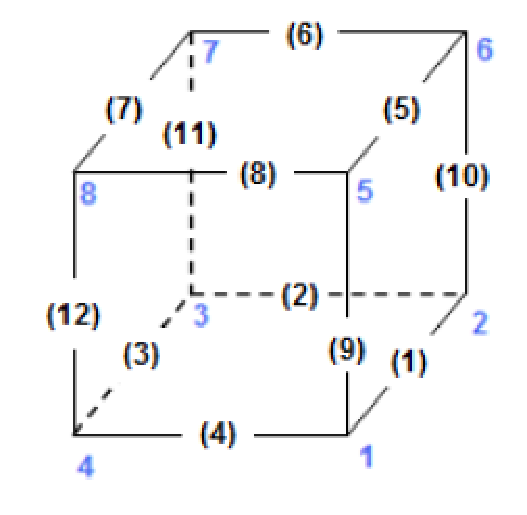
\includegraphics[scale=0.4]{Figs/3dcube}\label{fig:3dcube}}}
%{\begin{minipage}[c][1\width]{0.4\textwidth}\centering 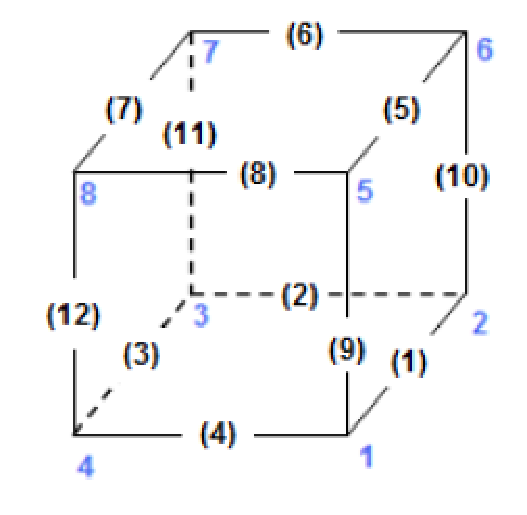
\includegraphics[width=0.4\textwidth]{Figs/3dcube} \end{minipage}}
\caption{Geometry description in .rea file}
\end{table}
\normalsize

\begin{figure}
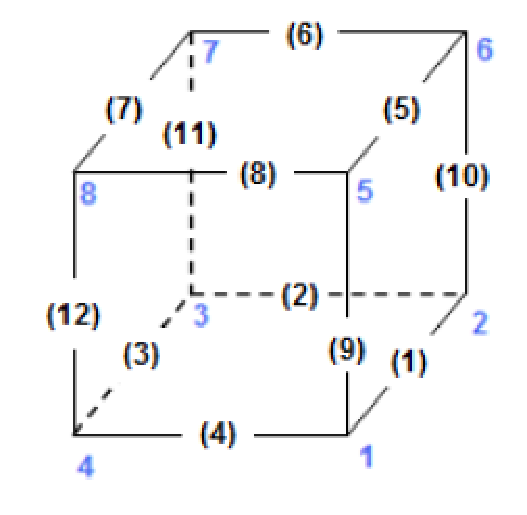
\includegraphics[scale=0.5]{Figs/3dcube}
\caption{Geometry description in .rea file (sketch of one element ordering)}
\end{figure}

\item{\bf curvature} 
     This section describes the deformation for elements that are curved.
     Currently-supported curved side or edge definitions include ``C''
     for circles, ``s'' for spheres, and ``m'' for midside-node positions
     associated with quadratic edge displacement. If no curved data is available the section remains empty.
     Example
     
     The section header may look like this 
     \begin{center}
     \texttt{640 Curved sides follow IEDGE,IEL,CURVE(I),I=1,5, CCURVE} 
     \end{center}
     and the data is stored as follows
  \footnotesize   
     \begin{center}
\begin{tabular}{ l|l|l|l|l }
   \hline
 \texttt{IEDGE}& \texttt{IEL} &\texttt{CURVE(12,1,IEL)} &\texttt{CURVE(12,2..5,IEL)}&\texttt{CCURVE(12,IEL)} \\ \hline \hline
  3&  1 &  1.0000  &      0.0000 &    C \\
  7 & 1 &  1.0000  &      0.0000 &    C\\
   \hline
\end{tabular}   
\end{center}
\normalsize
     The array \texttt{CCURVE} (char curve) holds a character denoting the type of curved boundary, while the array \texttt{CURVE} holds the actual information about the curved boundary. There are up to five available components in the \texttt{CURVE} array in case more information is needed by other implementations, that do not represent the default. We may have
     \begin{itemize}
     \item 'C' stands for circle and is given by the radius of the circle, thus filling in only the first component of the \texttt{CURVE(12,1,NEL)} 
     \item 'S' stands for sphere and is given by the radius and the center of the sphere, thus filling the first 4 components of the \texttt{CURVE(12,1\ldots 4,NEL)}
     \item 'M' is given by the coordinates of the midside-node, thus filling the first 3 components of the \texttt{CURVE(12,1\ldots 3,NEL)}, and leads to a second order reconstruction of the face.
     \end{itemize}
Both 'C' and 'S' types allow for a surface of as high order as the polynomial used in the spectral method, since they have an underlying analytical description, any circle arc can be fully determined by the radius and end points. However for the 'M' curved element descriptor the surface can be reconstructed only up to second order. This can be later updated to match the high-order polynomial after the GLL points have been distributed across the boundaries. In .usrdat2 the user can move the geometry to match the intended surface, followed by a call to the subroutine 'fixgeom' which can realign the point distribution in the interior of the element.

\item{\bf boundary conditions} 
     Boundary conditions (BCs) are specified for each face of each element,
     for each {\tt field} (velocity, temperature, passive scalar \#1, etc.).
     A common BC is {\tt P}, which indicates that an element face is 
     connected to another element to establish a periodic BC.   Many of the 
     BCs support either a constant specification or a user defined
     specification which
     may be an arbitrary function.   For example, a constant Dirichlet
     BC for velocity is specified by {\tt V}, while a user defined BC
     is specified by {\tt v}.   This upper/lower-case distinction is 
     used for all cases.   There are about 70 different types of boundary
     conditions in all, including free-surface, moving boundary, heat flux,
     convective cooling, etc.
     
      The section header may look like this 
     \begin{center}
     \texttt{ ***** FLUID   BOUNDARY CONDITIONS *****}

     \end{center}
     and the data is stored as follows
      \footnotesize   
     \begin{center}
\begin{tabular}{ l|l|l|l|l|l }
   \hline
 \texttt{CBC}& \texttt{IEL} &\texttt{IEDGE} &\texttt{CONN-IEL}&\texttt{CONN-IEDGE} & redundant\\ \hline \hline
  E   & 1 & 1 &  4.00000   &    3.00000  &     0.00000      \\
   ..   & .. & .. &  ..   &   .. &    ..      \\
   W  &  5 & 3 &  0.00000  &     0.00000  &     0.00000    \\
    ..   & .. & .. & ..   &   ..  &    ..      \\
   P  &  5 & 5  & 149.000 &      6.00000  &     0.00000 \\
   \hline
\end{tabular}   
\end{center}
\normalsize
     
\end{description}

\subsubsection*{ Output info} 
\begin{description}
\item{\bf restart conditions} 

     Here, one can specify a file to use as an initial condition.
     The initial condition need not be of the same polynomial order
     as the current simulation.   One can also specify that, for example,
     the velocity is to come from one file and the temperature from another.
     The initial time is taken from the last specified restart file, but 
     this can be overridden.
\item{\bf History points}

The following section defines history points in the {\tt .rea} file, see example {\tt vortex/r1854a.rea}, or {\tt shear4/shear4.rea}
\begin{verbatim}
0 PACKETS OF DATA FOLLOW\\
***** HISTORY AND INTEGRAL DATA *****\\
    56 POINTS. H code, I,J,H,IEL \\
UVWP    H     31     31   1   6\\
UVWP    H     31     31   31  6\\
UVWP    H     31     31   31  54\\
 "      "      "      "    "   "\\
\end{verbatim}

The {\tt "56 POINTS"} line needs to be followed by 56 lines of the type shown. However, in each of the following lines, which have the {\tt UVWP} etc., location is CRUCIAL, it
must be layed out exactly as indicated above\footnote{these lines contain character strings, they use formatted reads}, it is therefore advisable to refer to the examples {\tt vortex, shear4}.  If you want to pick points close to the center of element 1 and are running with lx1=10, say, you might choose {\tt UVWP H 5 5 5 1}. \footnote{the indicated point would really be at the middle of the element only if lx1=9}

The UVWP tells the code to write the 3 velocity components and pressure to the .sch file at
each timestep (or, more precisely, whenever {\tt mod(istep,iohis)=0}, where {\tt iohis=param(52))}.
Note that if you have more than one history point then they are written sequentially at each
timestep. Thus 10 steps in the first example with {\tt param(52)=2} would write {\tt (10/2)*56 = 280}
lines to the .sch file, with 4 entries per line. The "H" indicates that the entry corresponds to a requested history point. A note of caution: if the {\tt ijk} values (5 5 5 in the preceding example line) exceed {\tt lx1,ly1,lz1} of your SIZE file, then they are truncated to that value. For example, if {\tt lx1=10} for the data at the top (31 31 31) then the code will use {\tt ijk} of (10 10 10), plus the given element number, in identifying the history point. It is often useful to set {\tt ijk} to large values (i.e., > {\tt lx1}) because the endpoints of the spectral element mesh are invariant when {\tt lx1} is changed. 

\begin{comment}
7. A difficulty with the current nek history point specification is finding the requisite ijke (e=element
number) values that correlate to the point of interest. There is a way to do this in postx that
is relatively painless, but this is not useful for very large problems. (The approach is:
SET PLOT FORMAT
SCALAR
VALUES
PLOT
Follow the instructions and for each point requested, postx will write to the screen lines that
are similar to the above, ready to be pasted into the .rea file.)
8. When you run nek, it will write the coordinate information to the logfile on the first timestep
so that you can verify the point locations.
\end{comment}
\item{\bf output specifications} 
     Outputs are discussed in a separate section below.
\end{description}


\noindent
It is important to note that Nek5000 currently supports two input file
formats, ascii and binary.   The {\tt .rea} file format
described above is ascii.  For the binary format, all sections
of the .rea file having storage requirements that scale with 
number of elements (i.e., geometry, curvature, and boundary 
conditions) are moved to a second, {\tt .re2}, file and
written in binary.   The remaining sections continue to 
reside in the {\tt .rea} file.   The distinction between
the ascii and binary formats is indicated in the {\tt .rea}
file by having a negative number of elements.
There are converters, {\tt reatore2} and {\tt re2torea}, in the Nek5000
tools directory to change between formats.   The binary file
format is the default and important for {\tt I/O} performance when the
number of elements is large ( \(>\) 100000, say).

    
\subsection{Parameters}
\begin{itemize}  
\item $\rho$, the density, is taken to be time-independent and
  constant; however, in a multi-fluid system
  different fluids can have different value of constant density.
\item $\mu$, the dynamic viscosity can vary arbitrarily in
  time and space; it can also be a function of temperature
  (if the energy equation is included) and strain rate
  invariants (if the stress formulation is selected).
\item $\sigma$, the surface-tension coefficient can vary
  arbitrarily in
  time and space; it can also be a function of temperature
  and passive scalars.
\item $\overline{\beta}$, the effective thermal expansion
  coefficient, is
  assumed time-independent and constant.
\item ${\bf f}(t)$, the body force per unit mass term can
  vary with time, space, temperature and passive scalars.
\item $\rho c_{p}$, the volumetric specific heat, can vary
  arbitrarily with time, space and temperature.
\item $\rho L$, the volumetric latent heat of fusion at a front,
  is taken to be time-independent and constant; however,
  different constants can be assigned to different fronts.
\item $k$, the thermal conductivity, can vary with time,
  space and temperature.
\item $q_{vol}$, the volumetric heat generation, can vary with
  time, space and temperature.
\item $h_{c}$, the convection heat transfer coefficient, can vary
  with time, space and temperature.
\item $h_{rad}$, the Stefan-Boltzmann constant/view-factor product,
  can vary with time, space and temperature.
\item $T_{\infty}$, the environmental temperature, can vary
  with time and space.
\item $T_{melt}$, the melting temperature at a front, is taken
  with time and space; however, different melting temperature
  can be assigned to different fronts.
\end{itemize}
  
In the solution of the governing equations together with
the boundary and initial conditions, Nek5000 treats the
above parameters as pure numerical values; their
physical significance depends on the user's choice of units.
The system of units used is arbitrary (MKS, English, CGS,
etc.). However, the system chosen must be used consistently
throughout. For instance, if the equations and geometry
have been non-dimensionalized, the $\mu / \rho$ in the fluid
momentum equation is in fact
the inverse Reynolds number, whereas if the equations are
dimensional, $\mu / \rho$ represents the kinematic viscosity with
dimensions of $length^{2}/time$.
%\begin{comment}
\section{Data Layout}
\label{sec:data_layout}

Nek5000 was designed with two principal performance criteria in mind,
namely, {\em single-node} performance and {\em parallel} performance.

A key precept in obtaining good single node performance was to use,
wherever possible, unit-stride memory addressing, which is realized by
using contiguously declared arrays and then accessing the data in
the correct order.   Data locality is thus central to good serial 
performance.   To ensure that this performance is not compromised
in parallel, the parallel message-passing data model is used, in which
each processor has its own local (private) address space.  Parallel
data, therefore, is laid out just as in the serial case, save that there
are multiple copies of the arrays---one per processor, each containing 
different data.  Unlike the shared memory model, this distributed memory
model makes data locality transparent and thus simplifies the task of
analyzing and optimizing parallel performance.

Some fundamentals of Nek5000's internal data layout are given below.

\begin{enumerate}
\item
Data is laid out as  \(u_{ijk}^e = u(i,j,k,e)\) \\

{\tt   i=1,...,nx1   (nx1 = lx1)} \\
{\tt   j=1,...,ny1   (ny1 = lx1)} \\
{\tt   k=1,...,nz1   (nz1 = lx1} or 1, according to ndim=3 or 2) \\

{\tt   e=1,...,nelv}, where {\tt nelv} \(\le\) {\tt lelv}, and {\tt lelv} is the upper
                 bound on number of elements, {\em per processor}.


\item
 Fortran data is stored in column major order (opposite of C).

\item
 All data arrays are thus contiguous, even when {\tt nelv} \(<\) {\tt lelv}

\item Data accesses are thus primarily unit-stride (see chap.8 of DFM
   for importance of this point), and in particular, all data on
   a given processor can be accessed as, e.g.,


\begin{verbatim}
   do i=1,nx1*ny1*nz1*nelv
      u(i,1,1,1) = vx(i,1,1,1)
   enddo
\end{verbatim}

   which is equivalent but superior (WHY?) to:

\begin{verbatim}
   do e=1,nelv
   do k=1,nz1
   do j=1,ny1
   do i=1,nx1
      u(i,j,k,e) = vx(i,j,k,e)
   enddo
   enddo
   enddo
   enddo
\end{verbatim}


   which is equivalent but vastly superior (WHY?) to:

\begin{verbatim}
   do i=1,nx1
   do j=1,ny1
   do k=1,nz1
   do e=1,nelv
      u(i,j,k,e) = vx(i,j,k,e)
   enddo
   enddo
   enddo
   enddo
\end{verbatim}


\item All data arrays are stored according to the SPMD programming
   model, in which address spaces that are local to each processor
   are private --- not accessible to other processors except through
   interprocessor data-transfer (i.e., message passing).  Thus

\begin{verbatim}
   do i=1,nx1*ny1*nz1*nelv
      u(i,1,1,1) = vx(i,1,1,1)
   enddo
\end{verbatim}

   means different things on different processors and {\tt nelv} may
   differ from one processor to the next.  (By at most 1, WHY ?)


\item For the most part, low-level loops such as above are expressed in
   higher level routines only through subroutine calls, e.g.,:

\begin{verbatim}
   call copy(u,vx,n)
\end{verbatim}

   where {\tt n:=nx1*ny1*nz1*nelv}.   Notable exceptions are in places where
   performance is critical, e.g., in the middle of certain iterative
   solvers.

\end{enumerate}


%\subsection{Additional files}

\chapter{Geometry}\label{sec:geom}

Note that in case of any changes in the SIZE file, a recompilation is necessary.\\
\section{Setting up the geometry}
%\subsection{Rectangular geometries}
\subsection{Uniformly Distributed Mesh}

Suppose you wish to simulate flow through an axisymmetric pipe,
of radius $R=0.5$ and length $L=4$.  You estimate that you will
need 3 elements in radial ($y$) direction, and 5 in the $x$ direction,
as depicted in Fig. \ref{fig:mesh_axi1}.
This would be specified by the following input file (called {\em pipe.box})
to genbox:

\begin{verbatim}
axisymmetric.rea
2                      spatial dimension
1                      number of fields
#
#    comments:   This is the box immediately behind the 
#                refined cylinder in Ugo's cyl+b.l. run.
#
#
#========================================================
#
Box 1                         Pipe
-5 -3                         Nelx  Nely
0.0   4.0   1.0               x0  x1   ratio
0.0   0.5   1.0               y0  y1   ratio
v  ,O  ,A  ,W  ,   ,          BC's:  (cbx0, cbx1, cby0, cby1, cbz0, cbz1)
\end{verbatim}
\begin{figure}
\centering
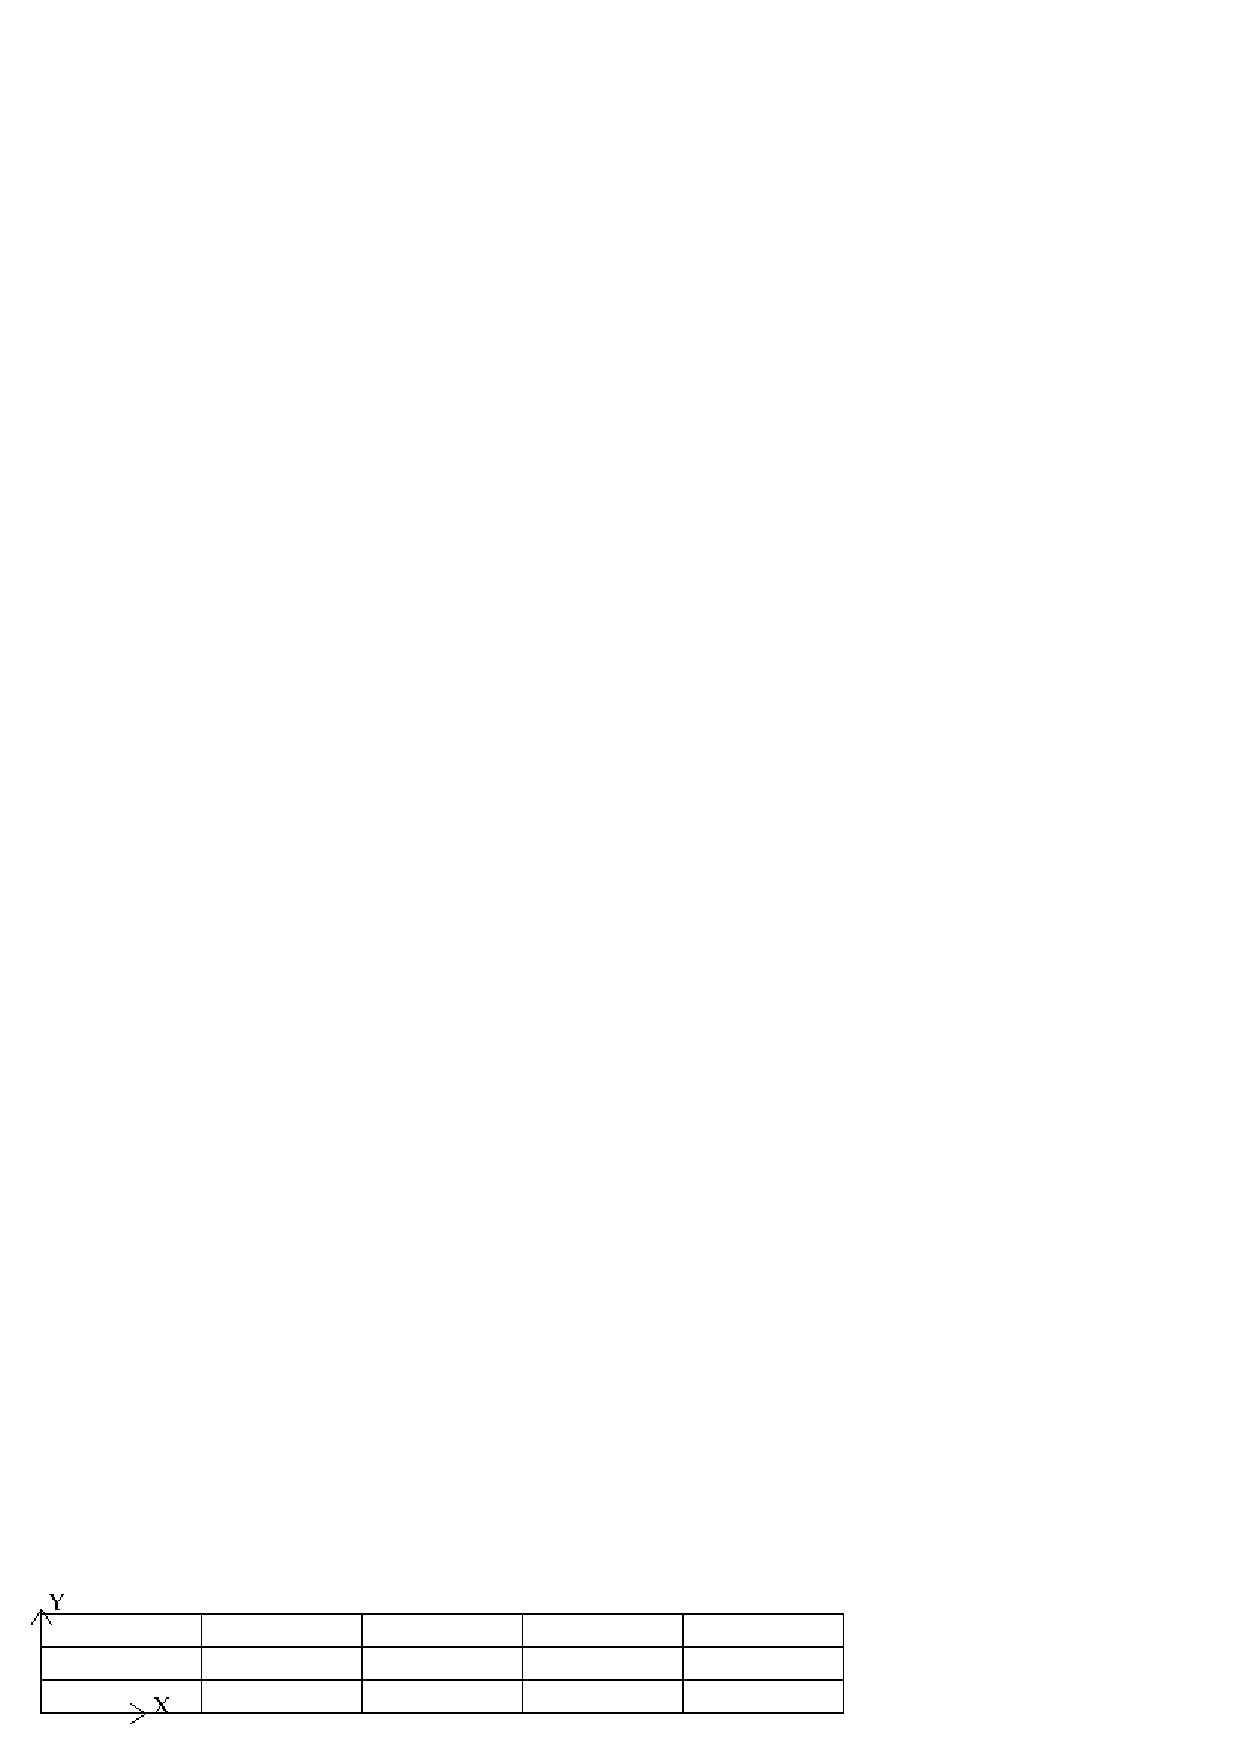
\includegraphics[width=0.8\textwidth]{Figs/mesh_axi1}
\caption{Axisymmteric pipe mesh}
\label{fig:mesh_axi1}
\end{figure}
\noindent
\begin{itemize}
\item
The first line of this file supplies the name of an existing 2D .rea file
that has the appropriate run parameters (viscosity, timestep size, etc.).
These parameters can be modified later, but it is important that 
axisymmetric.rea be a 2D file, and not a 3D file.
\item
The second line indicates the number of fields for this simulation, in
this case, just 1, corresponding to the velocity field (i.e., no heat 
transfer).
\item
The next set of lines just shows how one can place comments into a genbox
input file.
\item
The line that starts with ``Box'' indicates that a new box is starting,
and that the following lines describe a typical box input.  Other possible
key characters (the first character of Box, ``B'') are ``C'' and ``M'',
more on those later.
\item
The first line after ``Box'' specifies the number of elements in the
$x$ and $y$ directions.   The fact that these values are negative indicates
that you want genbox to automatically generate the element distribution 
along each axis, rather than providing it by hand.  (More on this below.)
\item
The next line specifies the distribution of the 5 elements in the $x$ direction.
The mesh starts at $x=0$ and ends at $x=4.0$.  The {\em ratio} indicates the
relative size of each element, progressing from left to right.  Here, 
\item
The next line specifies the distribution of the 3 elements in the $y$ direction,
starting at $y=0$ and going to $y=0.5$.  Again, 
{\em ratio}=1.0 indicates that the elements will be of uniform height.
\item
The last line specifies boundary conditions on each of the 4 sides of the
box:  
\begin{itemize}
\item
Lower-case {\em v} indicates that the left ($x$) boundary is to be a velocity
boundary condition, with a user-specified distribution determined by 
routine {\em userbc} in the .usr file.  (Upper-case $V$ would indicate that
the velocity is constant, with values specified in the .rea file.)
\item
{\em O} indicates that the right ($x$) boundary is an outflow boundary -- the
flow leaves the domain at the left and the default exit pressure is $p=0$.
\item
{\em A} indicates that the lower ($y$) boundary is the axis---this condition
is mandatory for the axisymmetric case, given the fact that the lower domain
boundary is at $y=0$, which corresponds to $r=0$.
\item
{\em W} indicates that the upper ($y$) boundary is a wall.  This would be
equivalent to a {\em v} or {\em V} boundary condition, with $\bu=0$.
\end{itemize}
\end{itemize}


\subsection{Graded Mesh}
\begin{figure}
\centering
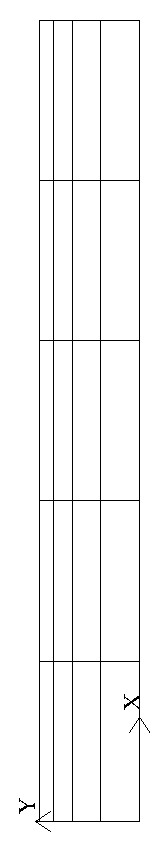
\includegraphics[width=0.8\textwidth]{Figs/mesh_axi2}
\caption{Axisymmteric pipe mesh, graded}
\label{fig:mesh_axi2}
\end{figure}

Suppose you wish to have the mesh be graded,
that you have increased resolution near the wall.
In this case you change {\em ratio} in the $y$-specification
of the element distribution.  For example, changing the 3 lines
in the above genbox input file from

\begin{verbatim}
-5 -3                         Nelx  Nely
0.0   4.0   1.0               x0  x1   ratio
0.0   0.5   1.0               y0  y1   ratio
\end{verbatim}

\noindent
to

\begin{verbatim}
-5 -4                         Nelx  Nely
0.0   4.0   1.0               x0  x1   ratio
0.0   0.5   0.7               y0  y1   ratio
\end{verbatim}

\noindent
yields the mesh shown in Fig. \ref{fig:mesh_axi2}.


\subsection{User-Specified Distribution}
\begin{figure}
\centering
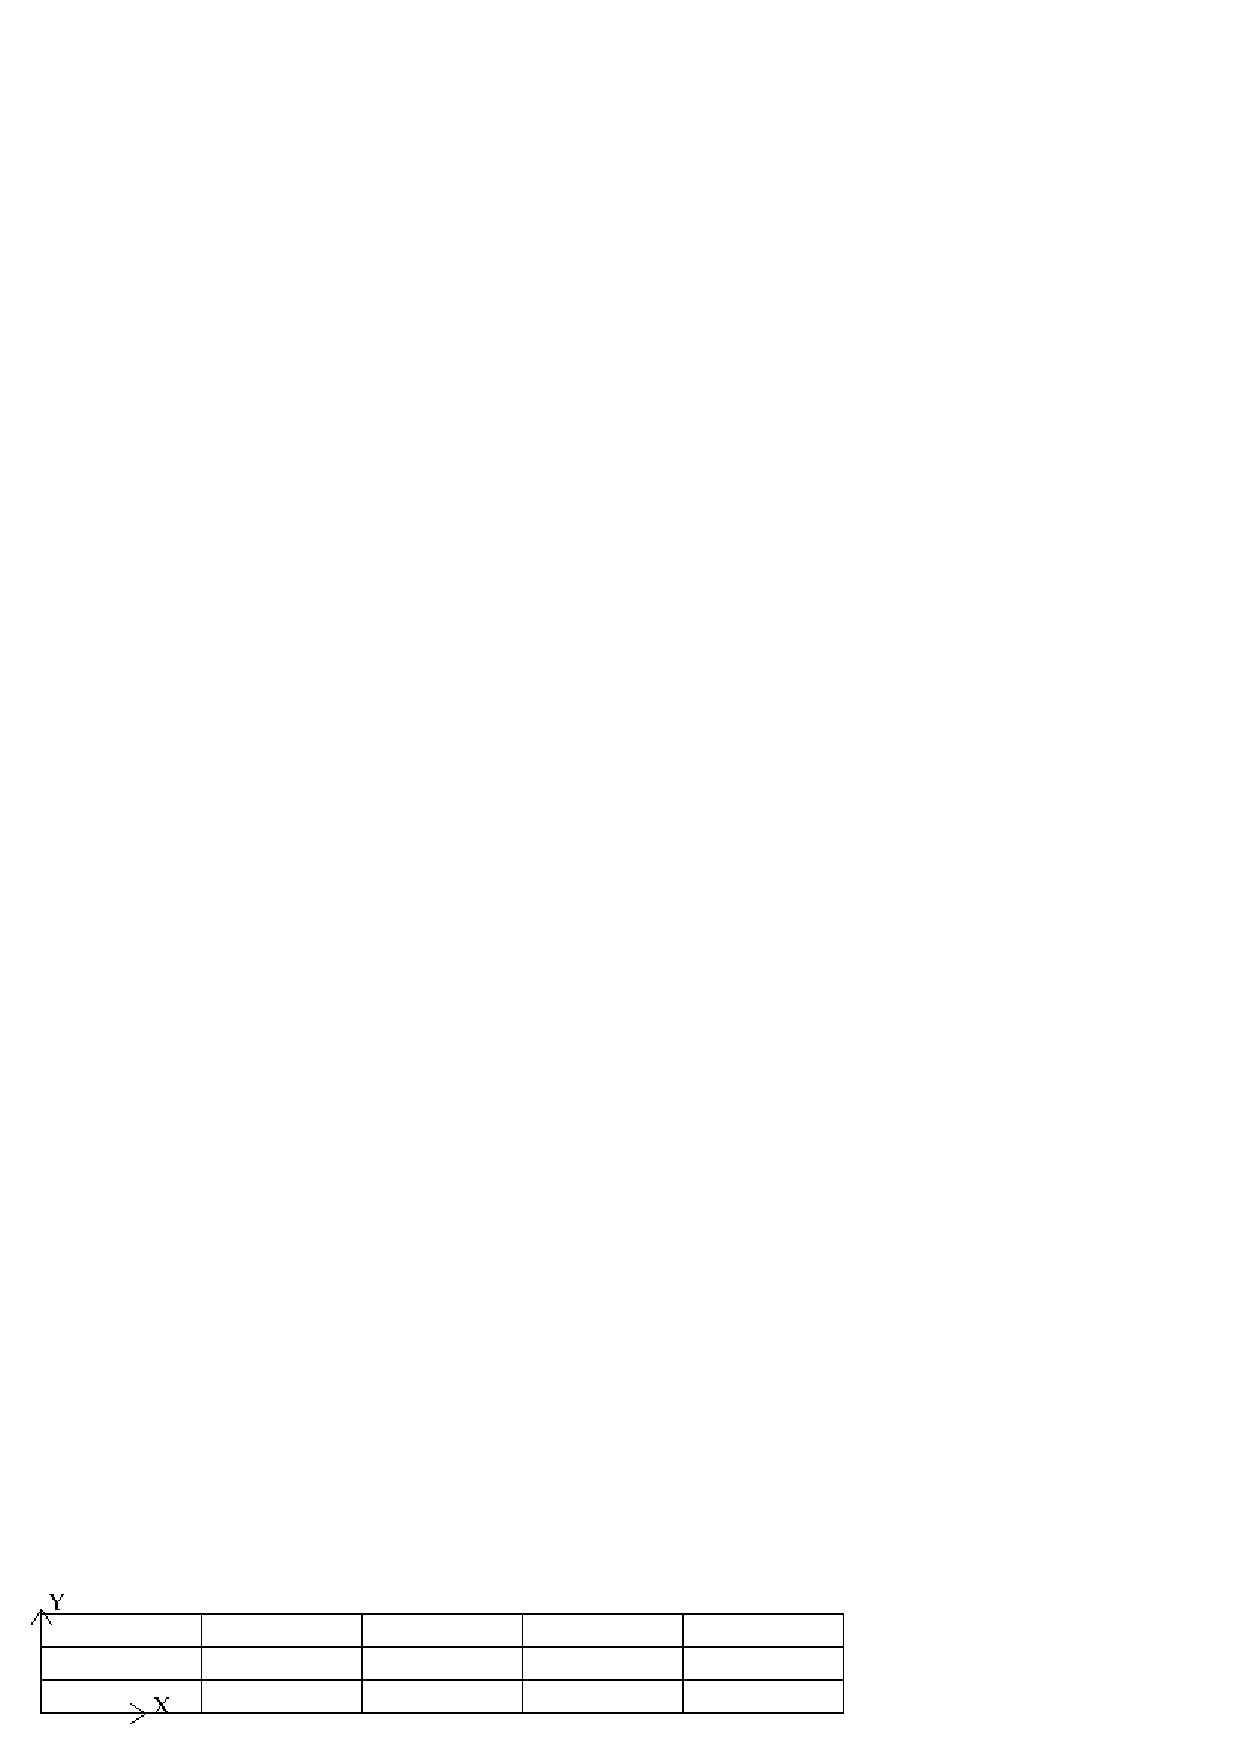
\includegraphics[width=0.6\textwidth]{Figs/mesh_axi1}
\caption{Axisymmteric pipe mesh, user specified}
\label{fig:mesh_axi1}
\end{figure}

You can also specify your own, precise, distribution of element
locations.   For example, another graded mesh similar to the
one of the preceding example could be built by changing the
genbox input file to contain:


\begin{verbatim}
-5  4                                               Nelx  Nely
0.0   4.0   1.0                                     x0  x1   ratio
0.000    0.250    0.375    0.450    0.500           y0  y1 ... y4
\end{verbatim}

\noindent
Here, the positive number of elements for the $y$ direction indicates
that genbox is expecting {\tt Nely+1} values of $y$ positions on the
$y$-element distribution line.   This is the genbox default, which
explains why it corresponds to {\tt Nely} $>$ 0.  The corresponding mesh
is shown in Fig. \ref{fig:mesh_axi3}.


\subsection{Mesh Modification in Nek5000}

For complex shapes, it is often convenient to modify the mesh
direction in the simulation code, Nek5000.  This can be done
through the usrdat2 routine provided in the .usr file.
The routine usrdat2 is called by nek5000 immediately after
the geometry, as specified by the .rea file, is established.
Thus, one can use the existing geometry to map to a new geometry
of interest.

For example, suppose you want the above pipe geometry to have
a sinusoidal wall.  Let $\bx := (x,y)$ denote the old geometry,
and $\bx' := (x',y')$ denote the new geometry.  For a domain
with $y\in [0,0.5]$, the following function will map the straight
pipe geometry to a wavy wall with amplitude $A$, wavelength $\lambda$:
\begin{eqnarray*}
y'(x,y) = y  + y A \sin( 2 \pi x / \lambda ).
\end{eqnarray*}
Note that, as $y \longrightarrow 0$, the perturbation, 
$yA \sin( 2 \pi x / \lambda )$, goes to zero.  So, near the axis,
the mesh recovers its original form.

In nek5000, you would specify this through usrdat2 as follows


\begin{verbatim}
      subroutine usrdat2
      include 'SIZE'
      include 'TOTAL'

      real lambda

      ntot = nx1*ny1*nz1*nelt

      lambda = 3.
      A      = 0.1

      do i=1,ntot
         argx         = 2*pi*xm1(i,1,1,1)/lambda
         ym1(i,1,1,1) = ym1(i,1,1,1) + ym1(i,1,1,1)*A*sin(argx)
      enddo

      param(59) = 1.  ! Force nek5 to recognize element deformation.

      return
      end
\end{verbatim}
\noindent
Note that, since nek5000 is modifying the mesh, postx will not
recognize the current mesh unless you tell it to, because postx
looks to the .rea file for the mesh geometry.  The only way for
nek5000 to communicate the new mesh to postx is via the .fld
file, so you must request that the geometry be dumped to the
.fld file.   This is done by modifying the OUTPUT SPECIFICATIONS,
which are found near the bottom of the .rea file.  Specifically,
change

\begin{verbatim}
  ***** OUTPUT FIELD SPECIFICATION *****
   6 SPECIFICATIONS FOLLOW
   F      COORDINATES
   T      VELOCITY
   T      PRESSURE
   T      TEMPERATURE
   F      TEMPERATURE GRADIENT
   0      PASSIVE SCALARS
\end{verbatim} 

\noindent
to

\begin{verbatim}
  ***** OUTPUT FIELD SPECIFICATION *****
   6 SPECIFICATIONS FOLLOW
   T      COORDINATES                       <------  CHANGE HERE
   T      VELOCITY
   T      PRESSURE
   T      TEMPERATURE
   F      TEMPERATURE GRADIENT
   0      PASSIVE SCALARS
\end{verbatim} 

\noindent
The result of above changes is shown in Fig. \ref{fig:wavypipe}.
\begin{figure}
\centering
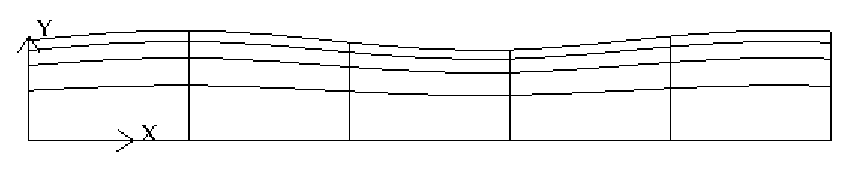
\includegraphics[width=0.8\textwidth]{Figs/wavypipe}
\caption{Axisymmteric pipe mesh}
\label{fig:wavypipe}
\end{figure}

\subsection{Cylindrical/Cartesian-transition Annuli}
\begin{figure}
\centering
\subfloat[Annuli mesh]{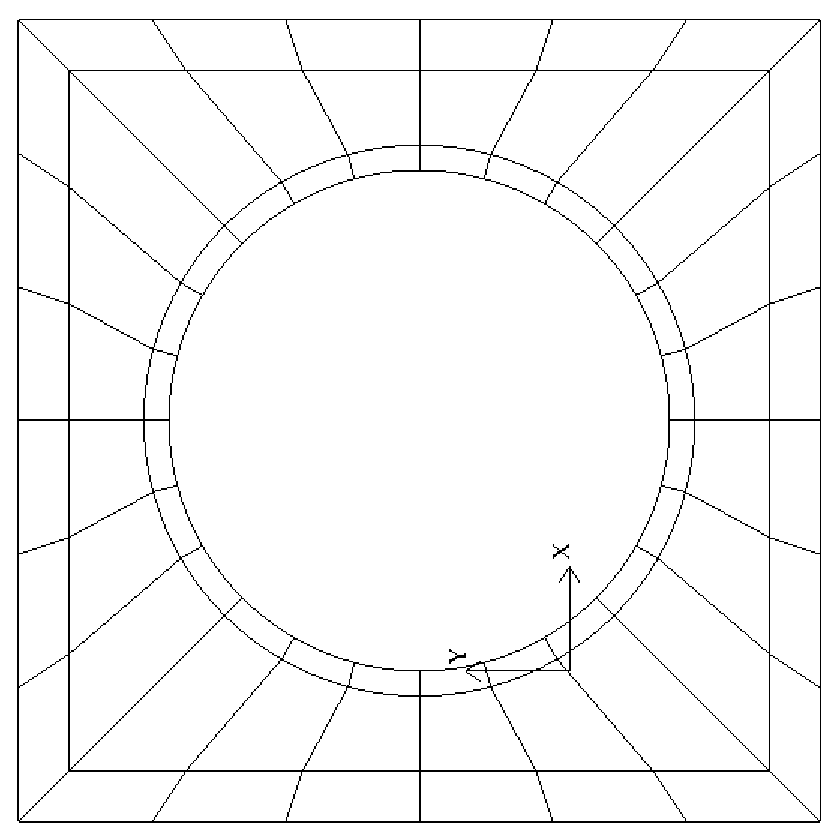
\includegraphics[width=0.3\textwidth]{Figs/cylbox_2d}\label{fig:cylbox_2d}}
\quad\quad\quad
\subfloat[Annuli mesh] {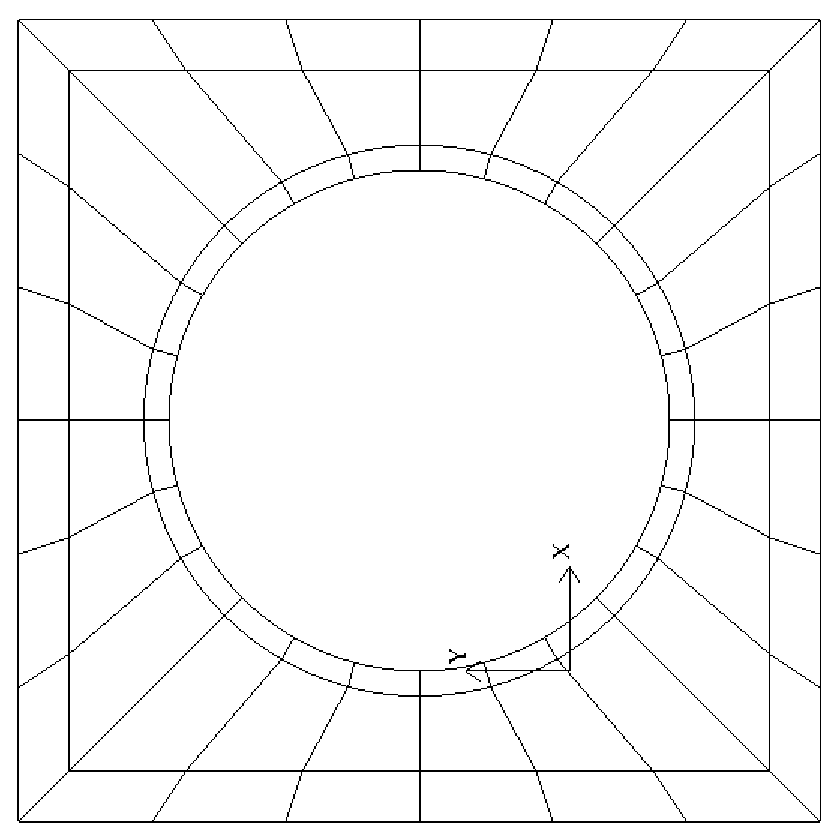
\includegraphics[width=0.3\textwidth]{Figs/cylbox_2d}\label{fig:cylbox_2da}} 
\caption{Cylinder mesh}
\end{figure}


An updated version of genb6, known as genb7, is currently under development
and designed to simply/automate the construction of cylindrical annuli, 
including {\em basic} transition-to-Cartesian elements.   More sophisticated
transition treatments may be generated using the GLOBAL REFINE options in
prenek or through an upgrade of genb7, as demand warrants.
Example 2D and 3D input files are provided in the nek5000/doc files
{\em box7.2d} and {\em box7.3d}.
Figure \ref{fig:cylbox_2d} shows a 2D example generated using 
the {\em box7.2d} input file, which reads:
\begin{verbatim}
x2d.rea
2                      spatial dimension
1                      number of fields
#
#    comments
#
#
#========================================================
#
Y                   cYlinder
3 -24 1             nelr,nel_theta,nelz
.5 .3               x0,y0 - center of cylinder
ccbb                descriptors: c-cyl, o-oct, b-box (1 character + space)
.5 .55 .7 .8        r0 r1 ... r_nelr
0  1  1             theta0/2pi theta1/2pi  ratio 
v  ,W  ,E  ,E  ,    bc's (3 characters + comma)
\end{verbatim}

\noindent
An example of a mesh is shown in Fig. \ref{fig:cylbox_2d}.   The mesh has been quad-refined
once with oct-refine option of prenek. The 3D counterpart to this 
mesh could joined to a hemisphere/Cartesian transition built with
the spherical mesh option in prenek. 
\label{sec:genbox}
%\input{mesh101}
%\section{Curvilinear geometry}
\section{Extrusion/Mirroring}
\subsection{Building Extruded Meshes with n2to3}

In nek5000/tools, there is a code n2to3.f that can be compiled with your
local fortran compiler (preferably not g77).
By running this code, you can extend two dimensional domains to
three dimensional ones with a user-specified number of levels in the
z-direction.  Such a mesh can then be modified using the mesh modification
approach. Assuming you have a valid two-dimensional mesh, n2to3 is straightforward
to run.  Below is a typical session, upon typing {\tt n2to3} the user is prompted at the command line

\begin{verbatim}
 Input old (source) file name:
h2e
 Input new (output) file name:
h3e
 input number of levels: (1, 2, 3,... etc.?):
16
 input z min:
0
 input z max:
16
 input gain (0=custom,1=uniform,other=geometric spacing):
1
 This is for CEM: yes or no:
n
 Enter Z (5) boundary condition (P,v,O):
v
 Enter Z (6) boundary condition (v,O):
0
 this is cbz: v  O   <---

      320 elements written to h3e.rea
FORTRAN STOP
\end{verbatim}

In this context CEM stands for computational electromagnetics, a spin-off of the original Nek5000 code.




The domain in which the fluid flow/heat transfer
problem is solved consists of two distinct subdomains. The
first subdomain is that part of the region occupied by
fluid, denoted \(\Omega_f\), while the second subdomain is that part
of the region occupied by a solid, denoted \(\Omega_s\). These two
subdomains are depicted in Fig.~\ref{fig:domains}. The entire domain is denoted as \(D=\Omega_f \cup \Omega_s\).
The fluid problem is solved in the domain \(\Omega_f\), while the
temperature in the energy equation is solved in the
entire domain; the passive scalars can be solved in either
the fluid or the entire domain.
  
We denote the entire boundary of \(\Omega_f\) as \(\partial \Omega_f\), that part
of the boundary of \(\Omega_f\) which is not shared by \(\Omega_s\) as
\(\overline{\partial \Omega_f}\), and
that part of the boundary of \(\Omega_f\) which is shared by \(\Omega_s\).
In addition, \(\partial \Omega_{s}, \overline{\partial \Omega_s}\) are analogously defined.
These distinct portions of the
domain boundary are illustrated in Fig.\ref{fig:domains}.
The restrictions on the domain for Nek5000 are itemized below.
\begin{itemize}
\item The domain \(\Omega=\Omega_f \cup \Omega_s\) must correspond either to a
  planar (Cartesian) two-dimensional geometry, or to the
  cross-section of an axisymmetric region specified by
  revolution of the cross-section about a specified axis, or
  by a (Cartesian) three-dimensional geometry.
\item For two-dimensional and axisymmetric geometries, the
  boundaries of both subdomains, \(\partial \Omega_f\) and
  \(\partial \Omega_s\), must be
  representable as (or at least approximated by) the union of
  straight line segments, splines, or circular arcs.
\item Nek5000 can interpret a two-dimensional image as either
  a planar Cartesian geometry, or
  the cross-section of an axisymmetric body. In the case of
  the latter, it is assumed that the y-direction is the radial
  direction, that is, the axis of revolution is at y=0.
  Although an axisymmetric geometry is, in fact,
  three-dimensional, Nek5000 can assume that the field variables
  are also axisymmetric ( that is, do not depend on azimuth,
  but only \(y\), that is, radius, \(x\), and \(t\) ), thus reducing the
  relevant equations to "two-dimensional" form.
\end{itemize}

Fully general three-dimensional meshes generated by other software
packages can be input to PRENEK as import meshes.
%\subsection{Description and implementation}
\section{Moving Geometry}
If the imposed boundary conditions allow for motion
of the boundary during the solution period (for example,
moving walls, free-surfaces, melting fronts, fluid layers),
then the geometry of the computational domain is automatically
considered in Nek5000 as being time-dependent.

For time-dependent geometry problems,
a mesh velocity {\bf w} is defined at each
collocation point of the computational domain (mesh) to
characterize the deformation of the mesh.
In the solution of the mesh velocity, the value of the mesh
velocity at the moving boundaries is first computed
using appropriate kinematic conditions (for free-surfaces, moving walls
and fluid layers) or dynamic conditions (for melting fronts).
On all other external boundaries, the normal mesh velocity on the
boundary is always set to zero.
In the tangential direction, either a zero tangential velocity
condition or a zero tangential traction condition is imposed; this
selection is automatically performed by Nek5000 based on
the fluid and/or thermal boundary conditions specified
on the boundary.
However, under special circumstances the user may want
to override the defaults set by Nek5000, this is
described in the PRENEK manual in Section 5.7.\footnote{This manual is old and may soon be deprecated.}
If the zero tangential mesh velocity is imposed, then the mesh
is fixed in space; if the zero traction condition is imposed,
then the mesh can slide along the tangential directions on
the boundary.
The resulting boundary-value-problem for the mesh velocity is solved
in Nek5000 using a elastostatic solver, with the Poisson ratio
typically set to zero.
The new mesh geometry is then computed by integrating the
mesh velocity explicitly in time and updating the nodal coordinates of the
collocation points.

Note that the number of macro-elements, the order of the macro-elements
and the topology of the mesh remain {\em unchanged} even though
the geometry is time-dependent.
The use of an arbitrary-Lagrangian-Eulerian description in Nek5000
ensures that the moving fronts are tracked with the minimum amount
of mesh distortion;
in addition, the elastostatic mesh solver can handle moderately
large mesh distortion.
However, it is the responsibility of the user to decide when
a mesh would become "too deformed" and thus requires remeshing.
The execution of the program will terminate when the mesh becomes
unacceptable, that is, a one-to-one mapping between the physical
coordinates and the isoparametric local coordinates for any
macro-element no longer exists.
\section{Boundary and initial conditions}

\subsection{Boundary Conditions}\label{sec:boundary}

The boundary conditions for the governing equations
given in the previous section are now described.
%Note that if the boundary conditions (for any field variable)
%are nonzero, the inhomogeneities can either be defined as constant, or as fortran functions of
%appropriate parameters such as space, time, temperature, etc.
%In this case, the user is responsible for using relevant variables in all
%fortran function definitions.

The boundary conditions can be imposed in various ways:
\begin{itemize}
\item when the mesh is generated with \texttt{genbox}, as will be explained in Section~\ref{sec:genbox}
\item when the .rea file is read in PRENEK or directly in the .rea file
\item directly in the .rea file
\item in the subroutine \texttt{userbc} 
\end{itemize} 

The general convention for boundary conditions in the .rea file is 
\begin{itemize}
\item upper case letters correspond to Primitive boundary conditions, as given in Table~\ref{tab:primitiveBCf, tab:primitiveBCt}
\item lower case letters correspond to user defined boundary conditions, see Table~\ref{tab:userBCf,tab:userBCt}
\end{itemize}

Since there are no supporting tools that will correctly populate the .rea file with the appropriate values, temperature, velocity, and flux boundary conditions are typically lower case and values must be specified in the \texttt{userbc} subroutine in the .usr file. %In this case PARAMs in the .rea file are dummies.
\subsection{Fluid Velocity}
  
Two types of boundary conditions are applicable to the
fluid velocity : essential (Dirichlet) boundary
condition in which the velocity is specified;
natural (Neumann) boundary condition in which the traction
is specified.
For segments that constitute the boundary \(\partial \Omega_f\), see Fig.~\ref{fig:domains},
one of these two types of boundary conditions must be
assigned to each component of the fluid velocity.
The fluid boundary condition can be {\em all Dirichlet}
if all velocity components of \(\bu\) are
specified; or it can be {\em all Neumann} if all traction components
\({\bf t} = [-p {\bf I} + \mu (\nabla \bu +
(\nabla \bu)^{T})] \cdot {\bf n}\), where
\({\bf I}\) is the identity tensor, \({\bf n}\) is the unit normal
and \(\mu\) is the dynamic viscosity, are specified;
or it can be {\em mixed Dirichlet/Neumann}
if Dirichlet and Neumann conditions are selected for different
velocity components.
Examples for all Dirichlet, all Neumann and mixed Dirichhlet/Neumann
boundaries are wall, free-surface and symmetry, respectively.
If the nonstress formulation is selected, then traction
is not defined on the boundary.
In this case, any Neumann boundary condition imposed must be homogeneous;
i.e., equal to zero.
In addition, mixed Dirichlet/Neumann boundaries must be aligned with
one of the Cartesian axes.

For flow geometry which consists of
a periodic repetition of a particular geometric unit,
the periodic boundary conditions can be imposed,
as illustrated in Fig.~\ref{fig:domains}.

\begin{table}
\begin{tabular}{ |l|l|l|l| }
   \hline
   Identifier & Description & Parameters&No of Parameters\\ \hline \hline
P    &   periodic                        &   periodic element and face & 2 \\
V    &   Dirichlet velocity              &   u,v,w                      &3 \\
O    &   outflow                         &   -                          &0  \\
W    &   wall (no slip)                  &   -                         & 0    \\                           
F    &   flux                            &   flux                      & 1\\
SYM  &   symmetry                        &   -                         & 0\\
A    &   axisymmetric boundary          &    -                         & 0\\
MS   &   moving boundary                 &   -                         & 0\\
ON   &   Outflow, Normal   &  -  &  0\\
E   &   Interior boundary   &  Neighbour element ID  &  2\\
   \hline
\end{tabular}
\caption{Primitive boundary conditions (flow velocity)}\label{tab:primitiveBCf}
\end{table}

\begin{table}
\begin{tabular}{ |l|l| }
   \hline
   Identifier & Description\\ \hline \hline
v  &      user defined Dirichlet velocity\\
t   &     user defined Dirichlet temperature\\
f    &    user defined flux\\
   \hline
\end{tabular}
\caption{User defined boundary conditions (flow velocity)}\label{tab:userBCf}
\end{table}
%\begin{itemize}
%\item 'MS ' (fs-hydro)
%\item 'O  ' 
%\item 'ON '    (blasius)
%\item 'S  '  (solid.rea)
%\end{itemize}

\paragraph*{}
The open(outflow) boundary condition ("O") arises as a natural boundary condition from the variational formulation of Navier Stokes. We identify two situations
\begin{itemize}
\item In the non-stress formulation, open boundary condition ('Do nothing')
\begin{equation}
[-p\vect I + \nu(\nabla \vect u)]\cdot \vect n=0
\end{equation}
\item In the stress formulation, free traction boundary condition
\begin{equation}
[-p\vect I + \nu(\nabla \vect u+\nabla \vect u^T)]\cdot \vect n=0
\end{equation}

\item the symmetric boundary condition ("SYM") is given as
\begin{eqnarray}
\vect u \cdot \vect n&=&0\ ,\\
(\nabla \vect u \cdot \vect t)\cdot \vect n&=&0
\end{eqnarray}
where \(\vect n\) is the normal vector and \(\vect t\) the tangent vector. If the normal and tangent vector are not aligned with the mesh the stress formulation has to be used.


\item the periodic boundary condition ("P") needs to be prescribed in the .rea file since it already assigns the last point to first via \(\vect u(\vect x)=\vect u(\vect x + L) \), where \(L\) is the periodic length.

\item the wall boundary condition ("W") corresponds to \(\vect u=0\).
\end{itemize}

%
%\begin{figure}
%\vspace{8.5in}
%\end{figure}
%
For a fully-developed flow in such a configuration, one can
effect great computational efficiencies by considering the
problem in a single geometric unit (here taken to be of
length L), and requiring periodicity of the field variables.
Nek5000 requires that the pairs of sides (or faces, in
the case of a three-dimensional mesh) identified as periodic
be identical (i.e., that the geometry be periodic).

For an axisymmetric flow geometry, the axis boundary
condition is provided for boundary segments that lie
entirely on the axis of symmetry.
This is essentially a symmetry (mixed Dirichlet/Neumann)
boundary condition
in which the normal velocity and the tangential traction
are set to zero.

For free-surface boundary segments, the inhomogeneous
traction boundary conditions
involve both the surface tension coefficient \(\sigma\)
and the mean curvature of the free surface.
\subsubsection{Passive scalars and Temperature}
  
The three types of boundary conditions applicable to the
temperature are: essential (Dirichlet) boundary
condition in which the temperature is specified;
natural (Neumann) boundary condition in which the heat flux
is specified; and mixed (Robin) boundary condition
in which the heat flux is dependent on the temperature
on the boundary.
For segments that constitute the boundary
\(\partial \Omega_f' \cup \partial \Omega_s'\) (refer to Fig. 2.1),
one of the above three types of boundary conditions must be
assigned to the temperature.

The two types of Robin boundary condition for temperature
are : convection boundary conditions for which the heat
flux into the domain depends on the heat transfer coefficient
\(h_{c}\) and the difference between the environmental temperature
\(T_{\infty}\) and the surface temperature; and radiation
boundary conditions for which the heat flux into the domain
depends on the Stefan-Boltzmann constant/view-factor
product \(h_{rad}\) and the difference between the fourth power
of the environmental temperature \(T_{\infty}\) and the fourth
power of the surface temperature.
\begin{table}
\begin{tabular}{ |l|l|l|l| }
   \hline
   Identifier & Description & Parameters&No of Parameters\\ \hline \hline
T    &   Dirichlet temperature/scalar    &   value                      &1 \\
O    &   outflow                         &   -                          &0  \\            
P    &   periodic boundary               &    -                         & 0\\
I    &   insulated (zero flux) for temperature&                        & 0\\
   \hline
\end{tabular}
\caption{Primitive boundary conditions (Temperature and Passive scalars)}\label{tab:primitiveBCt}
\end{table}

\begin{table}
\begin{tabular}{ |l|l| }
   \hline
   Identifier & Description\\ \hline \hline
t  &      user defined Dirichlet temperature\\
c   &     Newton cooling\\
f    &    user defined flux\\
   \hline
\end{tabular}
\caption{User defined boundary conditions (Temperature and Passive scalars)}\label{tab:userBCt}
\end{table}

\paragraph*{}
\begin{itemize}
\item open boundary condition ("O")
\begin{equation}
k(\nabla T)\cdot \vect n=0
\end{equation}
\item insulated boundary condition ("I")
\begin{equation}
k(\nabla T)\cdot \vect n=0
\end{equation}
where \(\vect n\) is the normal vector and \(\vect t\) the tangent vector. If the normal and tangent vector are not aligned with the mesh the stress formulation has to be used.

\item the periodic boundary condition ("P") needs to be prescribed in the .rea file since it already assigns the last point to first via \(\vect u(\vect x)=\vect u(\vect x + L) \), where \(L\) is the periodic length.

\item Newton cooling boundary condition ("c")
\begin{equation}
k(\nabla T)\cdot \vect n=h(T-T_{\infty})
\end{equation}
\item flux boundary condition ("f")
\begin{equation}
k(\nabla T)\cdot \vect n=f
\end{equation}
\end{itemize}

%\subsubsection*{Passive scalars}
The boundary conditions for the passive scalar fields
are analogous to those used for the temperature field.
Thus, the temperature boundary condition
menu will reappear for each passive scalar field so that the
user can specify an independent set of boundary conditions
for each passive scalar field. 


\subsection{Internal Boundary Conditions}

In the spatial discretization, the entire computational
domain is subdivided into macro-elements, the boundary
segments shared by any two of these macro-elements
in $\Omega_f$ and $\Omega_s$ are denoted as internal boundaries.
For fluid flow analysis with a single-fluid system or heat
transfer analysis without change-of-phase, internal
boundary conditions are irrelevant as the corresponding
field variables on these segments are part of the
solution. However, for a multi-fluid system and for
heat transfer analysis with change-of-phase, special
conditions are required at particular internal
boundaries, as described in the following.

For a fluid system composes of multiple immiscible fluids,
the boundary (and hence the identity) of each fluid must
be tracked, and a jump in the normal traction exists
at the fluid-fluid interface if the surface tension
coefficient is nonzero.
For this purpose, the interface between any two fluids
of different identity must be defined as a special type of
internal boundary, namely, a fluid layer;
and the associated surface tension coefficient also
needs to be specified.

In a heat transfer analysis with change-of-phase, Nek5000 assumes
that both phases exist at the start of the solution, and that
all solid-liquid interfaces are specified as special internal
boundaries, namely, the melting fronts.
If the fluid flow problem is considered, i.e., the energy
equation is solved in conjunction with the momentum and
continuity equations, then only
the common boundary between the fluid and the solid
(i.e., all or portion of $\partial \overline{\Omega}_f'$ in Fig.~\ref{fig:domains})
can be defined as the melting front.
In this case, segments on $\partial \overline{\Omega}_f'$ that
belong to the dynamic melting/freezing interface need to be
specified by the user.
Nek5000 always assumes that the density of the two phases
are the same (i.e., no Stefan flow); therefore at the melting
front, the boundary condition for the fluid velocity is the
same as that for a stationary wall, that is, all velocity
components are zero.
If no fluid flow is considered, i.e., only the energy equation
is solved, then any internal boundary can be defined as
a melting front.
The temperature boundary condition at the melting front
corresponds to a Dirichlet
condition; that is, the entire segment maintains a constant temperature
equal to the user-specified melting temperature $T_{melt}$
throughout the solution.
In addition, the volumetric latent heat of fusion $\rho L$
for the two phases,
which is also assumed to be constant, should be specified.

\subsection{Initial Conditions}

For time-dependent problems Nek5000 allows the user to choose among
the following types of initial conditions for the
velocity, temperature and passive scalars:
\begin{itemize}
\item Zero initial conditions: default; if nothing is specified.
\item Fortran function: This option allows the user to specify the
  initial condition as a fortran function,
  e.g., as a function of \(x\), \(y\) and \(z\).
\item Presolv: For a temperature problem the presolv option gives the
  steady conduction solution as initial condition for the temperature.
  For a fluid problem this option {\em can} give the
  steady Stokes solution as the initial condition for the velocity
  {\em provided} that the classical splitting scheme is {\em not} used.
\item Restart: this option allows the user to read in results from an earlier
  simulation, and use these as initial conditions.
\end{itemize}
A tabulated summary of the compatibility of these initial condition options
with various other solution strategies/parameters is given in the appendix.

\section{Mesh Partioning for Parallel Computing}
Genmap is spectral graph partitioning tool, similar to e.g. METIS, which partitions the graph associated to the mesh to assure optimal communication time in HPC applications. Let us consider a simple mesh such as the one in Fig.~\ref{fig:genmap}. The vertices are distributed in a random fashion, which is the way they may be provided by some mesh generator. Let us assume the vertices are here given as 
\[V_1=(-1,0),\ V_2=(0,1),\ V_3=(-1,2),\ V_4=(-1,1),\ V_5=(0,2),\ V_6=(0,0),\ V_7=(1,1),\ V_8=(1,0)\] 
The geometry is already stored in the .rea file by the point coordinates, and not vertex numbers
%\begin{table}
\begin{tabular}{c c c c}
%\fontsize 
  \(\texttt{Element } 1=[V_1\ V_6\ V_2\ V_4]\)&&&\\
  \(x_{1,\ldots,4}=\) -1. & 0. & 0. & -1.\\
  \(y_{1,\ldots,4}=\) 0.  & 0. & 1. &1.\\
  \(\texttt{Element } 2=[V_8\ V_7\ V_2\ V_6]\)&&&\\
  \(x_{1,\ldots,4}=\) 1. & 1. & 0. & 0.\\
  \(y_{1,\ldots,4}=\) 0. & 1. & 1. &0.\\
  \(\texttt{Element } 3=[V_5\ V_3\ V_4\ V_2]\)&&&\\
  \(x_{1,\ldots,4}=\) 0. & -1. & -1. & 0.\\
  \(y_{1,\ldots,4}=\) 2 .& 2.  & 1.  &1.\\
  \end{tabular}
%\end{table}

\begin{figure}
\centering
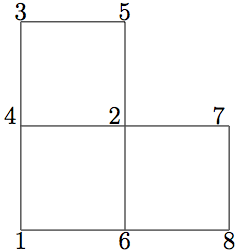
\includegraphics[scale=1]{genmap_sketch}
\caption{Two-dimensional mesh}
\label{fig:genmap}
\end{figure}

Let us a regard the mesh in Fig.~\ref{fig:genmap} as a graph of \(N\) vertices and \(M\) edges, \(G(V_N,E_M)\). We define the Laplacian matrix associated to a graph \(G\) as \(L(G)\). We define as the degree of a node \(V_i\) the number of incident edges, e.g. in Fig.~\ref{fig:genmap} \(deg(V_2)=4\) and \(deg(V_6)=3\).
\begin{equation}
L(G)_{ij}= \left\{
  \begin{array}{l l}
    i=j & \quad \mathrm deg(V_i)\\
    i\neq j & \quad -1 \text{ if there is and edge (i,j) and } 0 \text{ otherwise}
  \end{array} \right .
\end{equation}

\begin{equation}
L(G)= \begin{pmatrix} 
  &1 & 2 & 3 & 4 & 5 & 6 & 7 & 8\\ 
  \hline
1| &2 & 0 & 0 & -1 & 0 & -1 & 0 & 0\\ 
2| &0 & 4 & 0 & -1 & -1 & -1 & -1 & 0\\  
3| &0 & 0 & 2 & -1 & -1 & 0 & 0 & 0\\ 
4| &-1 & -1 & -1 & 3 & 0 & 0 & 0 & 0\\ 
5| &0 & -1 & -1 & 0 & 2 & 0 & 0 & 0\\ 
6| &-1 & -1 & 0 & 0 & 0 & 3 & 0 & -1\\ 
7| &0 & -1 & 0 & 0 & 0 & 0 & 2 & -1\\ 
8| &0 & 0 & 0 & 0 & 0 & -1 & -1 & 2\\  
\end{pmatrix}
\end{equation}

Properties of \(L(G)\)
\begin{itemize}
\item \(L(G)\) symmetric
\item the unit vector \(e=[1, \ldots 1]\in \mathcal{N}(L(G))\) is in the nullspace of the Laplacian matrix
\item \(\forall\lambda \in \sigma(L(G)>0\), i.e. all the eigenvalues of \(L(G)\) are positive except \(\lambda_0\) corresponding to the unit vector
\item \(\lambda_2\neq 0\) if the graph is connected, \(\lambda_2(L(G))\) is also called the algebraic connectivity of the graph
\end{itemize}

The main ides of the spectral bisection algorithm is
\begin{verbatim}
compute \(v_2\) eigenvector corresponding to \(\lambda_2(L(G))\)
for i=1,N
  if v_2(i) < 0 put vertex \(V_i\) in N_{-} 
  else put vertex \(V_i\) in N_{-} 
\end{verbatim}

The eigenvectors and eigenvalues are computed using Lanczos's algorithm.
These steps are repeated recursively on each of the two branches of the graph \(N_{-}, N_{+}\). This is possible since according to Fiedler's theorems the graph \(N_{-}\) is connected, \(N_{+}\) connected only if no \(v_2(i)=0\),  and for each subgraph \(G_1\) the algebraic connectivities satisfy \(\lambda_2(L(G_1))\leq\lambda_2(L(G))\).



To run the genmap code be sure that the Nek tools are up-to-date and compiled. 
At command line type: genmap 
NOTE-If the executables for the tools were not placed in the bin directory(default), 
include the path to the genmap executable. We give here the output for the .rea file in the Kovasznay example
\begin{verbatim}
Input (.rea) file name:
kov
Input mesh tolerance (default 0.2):
NOTE: smaller is better, but generous is more forgiving for bad meshes.
0.05
 reading .rea file data ...
 start locglob_lexico:           8         960        7680  0.10000000000000001     
 locglob:           1           1        7680
 .....
 locglob:           3        1254        7680
 done locglob_lexico:        1254        1254        7680           8
 start periodic vtx:         960        1254
 done periodic vtx
 start rec_bisect:         960
 done:    0.1% 
 .....
 done:   99.4% 
  
 done rec_bisect
writing kov.map    
\end{verbatim}
The user is prompted for .rea file name and should enter only the prefix of the .rea file. 
The user is prompted for mesh tolerance value. Typically a value of .05 is sufficient. Increasing or decreasing this value should make very little difference in the mesh generation. However, if given an error from genmap, the tolerance may need to be made slightly more generous. 

A successful genmap run will produce a .map file with the proper processor decomposition.


NOTE: For large element counts, it is not uncommon for genmap to be produce a few disconnected sets.  
These sets are typically under 7 elements large and  will not affect optimization of the NEK5000 run.  
If a disconnected set is produced, genmap will output the following warning to stdout.
\begin{verbatim}
 not connected   N0   NEL  Nsets   Nlarge sets
\end{verbatim}  
Here, {\tt N0} is the number of elements disconnected from the set of {\tt NEL} elements, {\tt Nsets} is the counter of disconnected sets found, 
and {\tt Nlarge sets} is the number of sets greater than 64 elements in size.  {\tt Nlarge sets} should always be 0.  If not, please contact someone on the developer team so we can be sure to have a more optimal partition of your mesh.

Genmap outputs an ordered set of numbers which are organized as follows
Line number 1 contains the header {\tt nel, nactive, depth, d2, npts, nrank, noutflow}

\begin{itemize}
\item {\tt nel}  number of elements
\item {\tt nactive} nrank-noutflow
\item {\tt depth} floor(log2(nel))
\item {\tt d2} \(2^{depth}\)
\item {\tt npts} number of corner points ({\tt nel*4} in 2D, {\tt nel*8} in 3D)
\item {\tt nrank} number of unique corner points
\item {\tt noutflow} number of outflows (not used anymore, is zero)
\end{itemize}

For the Kovasnay flow on an 8 element mesh with periodic boundary conditions we have
 {\tt 8         12          3          8         32         12          0}
 

Next we have the data (one line per element, listed in order of global element number)
====
{\tt 6          12          11           6           5}

This means that elemnt one (since we are on the first line) belongs to group 6, and this element is given by vertices in unique ordering. 
The vertices are ordered in symmetric ordering (starting at 1)

3 - 4
|   |
1 - 2

To distribute amongst processors, one just takes as many consecutive
processors as one wants.


\chapter{Performing large scale simulations  in Nek5000}
\section{Large scale simulations}
The largest simulations performed so far with Nek5000 are in the range of \(5\times 10^6\). 
Performance aspects to keep in mind
\begin{itemize}
\item design your SEM-mesh for a polynomial order N=7 or N=9 (lx1 in SIZE)
\item turn on dealiasing only if needed and try to minimize the polynomial order used for the fine grid (lxd in SIZE)
\item ensure that you have at least 50 elements per MPI process (the more the better)
\item explore the pressure solver performance using AMG solver (sweet spot depends on number of processors and elements)
\item make sure usrchk() does not contain time consuming operations getting called in the time loop
\item enable tuned MxM implementation for your platform (see makenek options)
\item turn on residual projection scheme (see .rea file parameters)
\item tune your pressure/velocity tolerances (e.g. use 5e-5 for pressure and 1e-8 for velocity solver) having in mind your overall accuracy
\item try to maximize the timestep, if needed turn on OIFS scheme with a target Courant number of around 2.0
\item use the parallel I/O (MPI-IO or custom kernel) to write checkpoints to disk
\item understand where you spend most of the time - turn on solver and MPI timings to monitor solver performance (see makenek options)
\end{itemize}



In such context it is recommendable to save the .rea file as a binary re2. 

Also for input/output it may be necessary to use MPI I/O. In this case the code has to be compiled with MPI I/O, i.e. the line PPLIST="MPIIO" in the makefile should not be commented. For output we may use iofiles, the parameter 65 in the .rea file specifies the number of directories and separate files that have to be created as specified by the user.

For large scale simulations the AMG solver is a better, faster choice for solving the Poisson problem (the default solver is XXT).

\subparagraph*{AMG solver}
The code should be compiled once with the settings \texttt{AMG=true}, \texttt{AMG\_ DUMP=true}. In the tools folder of Nek5000 we can find the AMG solver, a Matlab version for the moment which is subject to further integration in the main code. The user should run the script run which will read the AMG dump files and create new ones. The new files are now to be used in the code and with \texttt{AMG\_ DUMP} commented out the user should recompile and run his Nek5000 version.

The AMG solver is a 3 stage process. 

The first step will generate the files needed for the matlab code. Next matlab must run the setup code and generate a set of .dat files. Then nek can run with the .dat files and use the AMG pressure solver.

AMG dump stage

    Make sure {\tt IFAMG} and {\tt IFAMG\_ DUMP} in makenek are uncommented and set to true
    Run makenek clean, then makenek <casename>
    Run Nek (this will produce a set of *.dat files) 

MATLAB AMG stage

    Move the {\tt amgdmp\_ *.dat} files to {\tt nek5\_ svn/trunk/tools/amg\_ matlab}: 

    {\tt mv amgdmp*.dat ../../trunk/tools/amg\_ matlab}

    {\tt cd ../../trunk/tools/amg\_ matlab}

    Run the script: {\tt tools/amg\_ matlab/run} (this may take several hours and will produce set of files) 

AMG run stage

    Move all *.dat files produced back to your case directory: 

    {\tt mv *.dat /path/to/case/dir}

    Comment IFAMG\_ DUMP in makenek (IFAMG should still be set to TRUE)
    Run makenek clean, then run {\tt makenek <casename>}
    Run Nek (the generated AMG files will be read during the AMG setup phase) 

Notes on improving AMG results:

    To help speed up the matlab process, try running the 1st stage, the AMG dump stage, with {\tt lx1=3} in the SIZE file. Using a lower lx1 number will create a sparser matrix and thus a speedier matlab resolution. lx1 can be increased when ready to run the 2nd stage, the AMG run stage, after the .dat files are produced. 

    To increase accuracy in the AMG results, try tightening the tolerances in the run script, in {\tt trunk/tools/amg\_ matlab}. Specifically, the first tolerance (default set to 0.5). Lowering this (say, to 0.1), will increase the time the matlab code stage takes, but the result will be a faster convergence in the pressure solves of the AMG run stage. 

\subparagraph*{Size related issues}  

Large simulations require a high number of nodes and thus a high number of variables. So far Nek5000 supports by default 4 byte integers, however the node numbering for big meshes may exceed this size and 8 byte integers may be needed. How is this done?

If more than 9 passive scalars are needed

Exiting Nek5000 while a batch job in being executed should be done not using \texttt{"qdel"} but \texttt{echo -1 > ioinfo}. 

\subparagraph*{MAKENEK}
 The shell script makenek is designed to assist the compilation process of NEK5000. The script will create a makefile based on the user settings section in makenek. The GNU gmake utility is used to build NEK5000.
Available configurations options:
\begin{table}[tb!]
\caption[Makenek]
{Compiler options} 
\label{tab:bdms}
\begin{center}
\begin{tabularx}{\textwidth}{@{} c c c Y @{}} % use 'Y' for first column
 \hline\hline 
  name 	&values 	&default 	&description \\ \hline\hline 
  PPLIST &	string 	&&	list of pre-processor symbols (BG,MOAB,BLAS\_ MXM, MPIIO)  \\ \hline
IFMPI &	true,false &true &	use MPI (needed for a multiprocessor computation) \\ \hline
IFAMG\_ DUMP & 	true,false 	&false &	dump AMG pre-processing files  \\ \hline
IFAMG 	&true,false &	false &	use AMG as coarse grid solver for pressure preconditioner else XXT  \\ \hline
F77 	&string &	mandatory 	&Fortran compiler (e.g. MPI: mpif77)  \\ \hline
CC &	string &	mandatory 	&C compiler (e.g. MPI: mpicc)  \\ \hline
G& 	string 	&optional &	optional compilation flags  \\ \hline
OPT\_ FLAGS\_ STD7 &	string &	optional &	optimization flags for L1,L2,L3  \\ \hline
OPT\_ FLAGS\_ MAG &	string &	optional& 	optimization flags for L4 (highest opt level)  \\ \hline
SOURCE\_ ROOT &	string &	mandatory &	path of nek5000 source  \\ \hline
USR 	&string &	optional &	object list of additional files to compile (make intructions (makefile\_ usr.inc required)  \\ \hline
USR\_ LFLAGS &	string &	optional &	optional linking flags  \\ \hline
MOAB\_ DIR &	string 	&NEK with MOAB &	Path to MOAB directories  \\ \hline
IFVISIT 	&true,false &	false 	&Toggles Visit in situ. See Visit\_ in\_ situ for details  \\ \hline
VISIT\_ INSTALL &	string &VISIT in situ &	Path to VISIT install path. See Visit\_ in\_ situ for details.  \\ \hline
VISIT\_ STOP 	&true,false &	false 	&When running VISIT in situ, simulation stops after step 1 to connect VISIT.  \\
 \hline\hline
\end{tabularx}
\end{center}
\end{table}



\subparagraph*{Binary geometry}
 Reatore2
Jump to: navigation, search

The NEK5000 tool, reatore2 allows users to split an ASCII .rea file to an ASCII .rea and a binary .re2 file. The .re2 file contains the mesh and boundary condition data that is normally written in ASCII in the .rea file. For large simulations, this information can be substantial, so storing it in binary lowers the memory footprint for the simulation.
Running reatore2

    Be sure that your nekton tools are up-to-date and compiled.
    At the command prompt type: reatore2 

NOTE-If the executables for the tools were not placed in the bin directory(default), 
include the path to the reatore2 executable

    User is prompted for name of .rea file 

    -Enter the name to the .rea file, excluding the .rea extenstion 

    User is prompted for the new files name 

    -Enter the name for your new files 



\section{Parallelism in Nek5000}



The parallelism of Nek5000 is accomplished via domain decomposition methods and a suitable gather-scatter code. All this is implemented in such way that the user does not have to be concerned with the parallelism and only focus on the actual solvers while keepin in mind a few simple rules and routines that switch from local to global and back.
\begin{itemize}
\item Locally, the SEM is structured.

\item Globally, the SEM is unstructured.

\item Vectorization and serial performance derive from the structured aspects of the computation.

\item Parallelism and geometric flexibility derive from the unstructured, element-by-element, operator evaluation.

\item Elements, or groups of elements are distributed across processors, but an element is never subdivided.
\end{itemize}

For the most part, the global element numbering is not relevant since Nek5000 assigns it randomly but following certain rules. 

There are two types of array sizes, starting with {\color{red}l}x1, {\color{red}l}elv, etc. which give an upper bound of the arrays. And {\color{red}n}x1, {\color{red}n}elv, etc. which give the actual number of elements/grid points per processors. For the example in Fig.~\ref{fig:procsplit} we have 
\begin{itemize}
\item on proc 0, {\tt nelt=2}  (nelt = no elements in temperature domain)
\item on proc 1, {\tt nelt=3}  (nelv = no elements in fluid domain, usually = nelt)
\end{itemize}

\begin{figure}
\centering
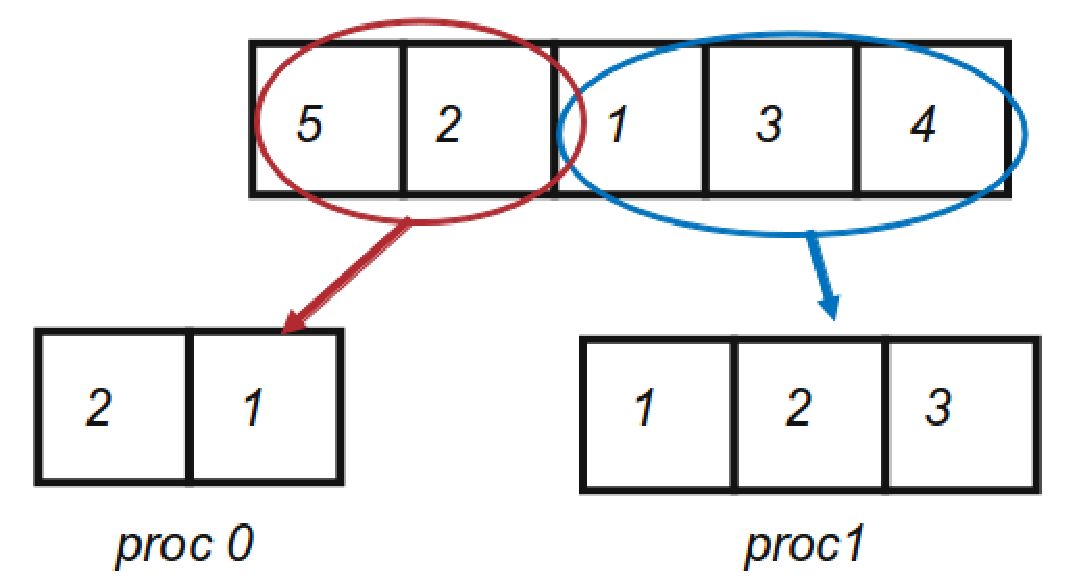
\includegraphics[scale=0.5]{Figs/serial_parallel}
\caption{A simple SEM row of elements and a potential splitting}
\label{fig:procsplit}
\end{figure}
Arrays {\tt lglel} that distinguish which processor has which elements, 

\begin{itemize}
\item on proc 0, {\tt nelt=2, lglel=(2,5)}, local element {\tt 1->2} and {\tt 2->5}
\item on proc 1, {\tt nelt=3, lglel=(1,3,4)}, local element {\tt 1->1}, {\tt 2->3} and {\tt 4->3}
\end{itemize}
		  
Now for global to local we have two common arrays (scaling as {\tt nelgt}, but only two such arrays)

\begin{itemize}
\item {\tt gllel=(1,1,2,3,2)}, assigns a global element to its local correspondent, i.e. global element {\tt 1->1}, {\tt 2->1} and {\tt 3->2} etc.
\item {\tt gllnid=(1,0,1,1,0)}, assigns a global element to its processor, i.e. {\tt 1->1}, {\tt 2->0} and {\tt 3->1} etc.
\end{itemize}



All data contiguously packed (and quad-aligned) {\tt real  u(lx1,ly1,lz1,lelt)} indicates that {\tt u} is a collection of elements, {\tt e=1,\(\ldots\),Nelt =< lelt}, each of size \((N+1)d, d=2 or 3\).

\textbf{Example: Summation}

Serial version
{\tt
s = 0 \\
do e=1,nelv \\
do iz=1,nz1 \\
do iy=1,ny1 \\
do ix=1,nx1 \\
s=s+u(ix,iy,iz,e) \\
enddo,\(\ldots\),enddo}

Second approach, serial version (works in parallel in Nek)
{\tt
n=nx1*ny1*nz1*nelv \\
s=0 \\
do i=1,n \\
s=s+u(i,1,1,1) \\
enddo
}

Nek Parallel Version

{\tt s=glsum(s,n)}

If you want a local max {\tt s=vlmax(u,n)}, or a global max {\tt s=glmax(u,n)}.



%\end{comment}
%\begin{comment}

\chapter{Routines of interest}
The most common routines needed in nek500 are
\subsection{Naming conventions}
\begin{itemize}
\item  {\tt{subroutine f(a,b,c)}}
a- returned variable
b,c -input data
\item {\tt{op}[]} represent operations on operators
\item {\tt{c}[]}  operations on constants
\item {\tt{gl}[]} global operations
\item {\tt{col2}[]} ---
\item {\tt{col3}[]} --
\end{itemize}

\subsection{Subroutines}
{\tt subroutine rescale\_x(x,x0,x1)}

    Rescales the array x to be in the range (x0,x1). This is usually called from usrdat2 in the .usr file 
    
{\tt subroutine normvc(h1,semi,l2,linf,x1,x2,x3)}

    Computes the error norms of a vector field variable(x1,x2,x3) defined on mesh 1, the velocity mesh. The error norms are normalized with respect to the volume, with the exception on the infinity norm, linf. 
    
{\tt subroutine comp\_vort3(vort,work1,work2,u,v,w)}

    Computes the vorticity (vort) of the velocity field, (u,v,w) 
    
{\tt subroutine lambda2(l2)}

    Generates the Lambda-2 vortex criterion proposed by Jeong and Hussain (1995) 
    
{\tt subroutine planar\_average\_z(ua,u,w1,w2)}

    Computes the r-s planar average of the quantity u. 
    
{\tt subroutine torque\_calc(scale,x0,ifdout,iftout)}

    Computes torque about the point x0. Here scale is a user supplied multiplier so that the results may be scaled to any convenient non-dimensionalization. Both the drag and the torque can be printed to the screen by switching the appropriate ifdout(drag) or iftout(torque) logical. 
    
{\tt subroutine set\_obj}

    Defines objects for surface integrals by changing the value of hcode for future calculations. Typically called once within userchk (for istep = 0) and used for calculating torque. (see above) 
    
{\tt subroutine avg1(avg,f, alpha,beta,n,name,ifverbose)}

{\tt subroutine avg2(avg,f, alpha,beta,n,name,ifverbose)}

{\tt subroutine avg3(avg,f,g, alpha,beta,n,name,ifverbose)}

    These three subroutines calculate the (weighted) average of f. Depending on the value of the logical, ifverbose, the results will be printed to standard output along with name. In avg2, the f component is squared. In avg3, vector g also contributes to the average calculation. 
    
{\tt subroutine outpost(x,vy,vz,pr,tz,' ')}

    Dumps the current data of x,vy,vz,pr,tz to an {\tt .fld} or {\tt .f0????} file for post processing. 
    
{\tt subroutine platform\_timer(ivrb)}

    Runs the battery of timing tests for matrix-matrix products,contention-free processor-to-processor ping-pong tests, and {\tt mpi\_all\_reduce} times. Allows one to check the performance of the communication routines used on specific platforms. 
    
{\tt subroutine quickmv}

    Moves the mesh to allow user affine motion. 
    
{\tt subroutine runtimeavg(ay,y,j,istep1,ipostep,s5)}

    Computes,stores, and (for ipostep!0) prints runtime averages of j-quantity y (along w/ y itself unless ipostep<0) with j + 'rtavg\_' + (unique) s5 every ipostep for istep>=istep1. s5 is a string to append to rtavg\_ for storage file naming. 
    
{\tt subroutine lagrng(uo,y,yvec,uvec,work,n,m)}

    Compute Lagrangian interpolant for uo 
    
{\tt subroutine opcopy(a1,a2,a3,b1,b2,b3)}

    Copies b1 to a1, b2 to a2, and b3 to a3, when ndim = 3, 
    
{\tt subroutine cadd(a,const,n)}

    Adds const to vector a of size n. 
    
{\tt subroutine col2(a,b,n)}

    For n entries, calculates a=a*b. 
    
{\tt subroutine col3(a,b,c,n)}

    For n entries, calculates a=b*c. 
\subsection{Functions}

{\tt function glmax(a,n)}
{\tt function glamax(a,n)}
{\tt function iglmax(a,n)}
    Calculates the (absolute) max of a vector that is size n. Prefix i implies integer type. 
{\tt function i8glmax(a,n)}
    Calculates the max of an integer*8 vector that is size n. 
{\tt function glmin(a,n)}
{\tt function glamin(a,n)}
{\tt function iglmin(a,n)}
    Calculates the (absolute) min of a vector that is size n. Prefix i implies integer type. 


{\tt function glsc2(a,b,n)}
{\tt function glsc3(a,b,mult,n)}
{\tt function glsc23(z,y,z,n)}
    Performs the inner product in double precision. glsc3 uses a multiplier, mult and glsc23 performs x*x*y*z. 


{\tt function glsum(x,n)}
{\tt function iglsum(x,n)}
{\tt function i8glsum(x,n)}
    Computes the global sum of x, where the prefix, i specifies type integer, and i8 specifies type integer*8. 

\subsection{An example of specifying surface normals in the .usr file}
\begin{verbatim}

c-----------------------------------------------------------------------
      subroutine userbc (ix,iy,iz,iside,eg)
      include 'SIZE'
      include 'TOTAL'
      include 'NEKUSE'

      integer e,eg,f
      real snx,sny,snz   ! surface normals

      f = eface1(iside)
      e = gllel (eg)

      if (f.eq.1.or.f.eq.2) then      ! "r face"
         snx = unx(iy,iz,iside,e)                 ! Note:  iy,iz
         sny = uny(iy,iz,iside,e)
         snz = unz(iy,iz,iside,e)
      elseif (f.eq.3.or.f.eq.4)  then ! "s face"
         snx = unx(ix,iz,iside,e)                 !        ix,iz
         sny = uny(ix,iz,iside,e)
         snz = unz(ix,iz,iside,e)
      elseif (f.eq.5.or.f.eq.6)  then ! "t face"
         snx = unx(ix,iy,iside,e)                 !        ix,iy
         sny = uny(ix,iy,iside,e)
         snz = unz(ix,iy,iside,e)
      endif

      ux=0.0
      uy=0.0
      uz=0.0
      temp=0.0

      return
      end
\end{verbatim}  

This example will load a list of field files (filenames are read from a file) into the solver using the {\tt load\_fld()} function. After the data is loaded, the user is free to compute other postprocessing quantities. At the end the results are dumped onto a regular (uniform) mesh by a subsequent call to prepost().

Note: The regular grid data (field files) cannot be used as a restart file (uniform->GLL interpolation is unstable)!

\begin{verbatim}


     SUBROUTINE USERCHK
     INCLUDE 'SIZE'
     INCLUDE 'TOTAL'
     INCLUDE 'RESTART' 

     character*80 filename(9999)

     ntot   = nx1*ny1*nz1*nelv

     ifreguo = .true.   ! dump on regular (uniform) grid instead of GLL
     nrg     = 16       ! dimension of regular grid (nrg**ndim)
 
     ! read file-list
     if (nid.eq.0) then
        open(unit=199,file='file.list',form='formatted',status='old')
        read(199,*) nfiles
        read(199,'(A80)') (filename(i),i=1,nfiles)
        close(199)
     endif
     call bcast(nfiles,isize)
     call bcast(filename,nfiles*80)       

     do i = 1,nfiles
        call load\_ fld(filename(i))

        ! do something
        ! note: make sure you save the result into arrays which are
        !       dumped by prepost() e.g. T(nx1,ny1,nz1,nelt,ldimt)
        ...

        ! dump results into file
        call prepost(.true.,'his')
     enddo

     ! we're done
     call exitt

\end{verbatim}

\subsection{Spectral Interpolation Tool}

{\tt Check intpts().}
Monitor Points

Multiple monitor points can be defined in the file hpts.in to examine the field data at every timestep.

\begin{itemize}
\item setup an ASCII file called 'hpts.in' e.g: 
\begin{verbatim}
3 !number of monitoring points
1.1 -1.2 1.0
. . .
x y z
\end{verbatim}

\item depending on the number number of monitoring points you may need to increase {\tt lhis} in SIZE.
\item    add {\tt 'call hpts()'} to {\tt userchk()} 
\end{itemize}

\subsection{Grid to Grid Interpolation}

To interpolate an existing field file (e.g. base.fld) onto a new mesh do the following:
\begin{itemize}
\item set lpart in SIZE to a large value (e.g. 100'000 or larger) depending on your memory footprint
\item    compile Nek with MPIIO support
\item    set NSTEPS=0 in the .rea file (post-processing mode)
\item    run nek using the new geometry (e.g. new\_geom.f0000)
\item    run nek using the old geometry and add this code snipplet to userchk() 
\begin{verbatim}
 character*132  newfld, oldfld, newgfld
 data newfld, oldfld, newgfld /'new0.f0001','base.fld','new\_geom.f0000'/
 call g2gi(newfld, oldfld, newgfld) ! grid2grid interpolation
 call exitt()
\end{verbatim}
\end{itemize}
    

\subsection{Lagrangian Particle Tracking}

The interpolation tool can be used for Lagrangian particle tracking (the particles are the interpolation points).

Workflow: Set initial particle positions (e.g. reading a file particle.pos0) x\_part <- x\_pos0 

LOOP
\begin{itemize}
 \item    compute field quantities
\item    interpolate field quantities for all particles using intpts()
\item    dump/store particle data
\item    advect particles using particle\_advect()
\end{itemize}
END LOOP
\begin{verbatim}
    subroutine particle\_ advect(rtl,mr,npart,dt\_ p)
c     
c     Advance particle position in time using 4th-order Adams-Bashford.
c     U[x\_ i(t)] for a given x\_ i(t) will be evaluated by spectral interpolation.
c     Note: The particle timestep dt\_ p has be constant!
c
     include 'SIZE'
     include 'TOTAL'
        
     real rtl(mr,1)
         
     real vell(ldim,3,lpart)  ! lagged velocities 
     save vell
        
     integer icalld
     save    icalld
     data    icalld /0/
        
     if(npart.gt.lpart) then
       write(6,*) 'ABORT: npart>lpart - increase lpart in SIZE. ',nid
       call exitt
     endif 
        
    ! compute AB coefficients (for constant timestep)
     if (icalld.eq.0) then
        call rzero(vell,3*ldim*npart) ! k = 1 
        c0 = 1.
        c1 = 0.
        c2 = 0.
        c3 = 0.                       
        icalld = 1
     elseif (icalld.eq.1) then        ! k = 2
        c0 = 1.5
        c1 = -.5
        c2 = 0.
        c3 = 0.
        icalld = 2
     elseif (icalld.eq.2) then        ! k = 3
        c0 = 23.
        c1 = -16.
        c2 = 5.
        c0 = c0/12.
        c1 = c1/12.
        c2 = c2/12.
        c3 = 0.
        icalld = 3
     else                             ! k = 4
        c0 = 55.
        c1 = -59.
        c2 = 37.
        c3 = -9.
        c0 = c0/24.
        c1 = c1/24.
        c2 = c2/24.
        c3 = c3/24.
     endif

     ! compute new position x[t(n+1)]
     do i=1,npart
        do k=1,ndim
           vv = rtl(1+2*ndim+k,i)
           rtl(1+k,i) =  rtl(1+k,i) +
    \&                    dt\_p*(
    \&                    + c0*vv
    \&                    + c1*vell(k,1,i)
    \&                    + c2*vell(k,2,i)
    \&                    + c3*vell(k,3,i)
    \&                    )
           ! store velocity history 
           vell(k,3,i) = vell(k,2,i)
           vell(k,2,i) = vell(k,1,i)
           vell(k,1,i) = vv
        enddo
     enddo

     return
     end
  \end{verbatim}  

%\section{Troubleshooting}
%\input{troubleshoot}
\begin{comment}
\chapter{Postprocessing}
\section{Visualisation}
%\section{Toolboxes}

%\chapter{Algorithms}
%\section{Flow solvers}
%\section{Filtering}
\end{comment} 
\chapter{Appendix}
\section{Appendix A. Extensive list of parameters .rea file}
\subsection{Parameters}
This section tells nek5000
\begin{itemize}
\item If the input file reflects a 2D or 3D job (it should match the \textit{ldim} parameter in the SIZE file).
\item The combination of heat transfer, Stokes, Navier-Stokes, steady or unsteady to be run.
\item The relevant physical parameters.
\item The solution algorithm within nek5000 to use.
\item The timestep size or Courant number to use, or whether to run variable DT (\(dt\)), etc.
\end{itemize}
A .rea file starts with the following three parameters:
\begin{description}
\item [NEKTON VERSION] the version of nek5000
\item [DIMENSIONAL RUN] number of spatial dimensions (NDIM=2,3 - has to match the setting in the SIZE file).
\item [PARAMETERS FOLLOW] the number of parameters which are going to be followed in the .rea file.(NPARAM)
\end{description}
The latter specifies how many lines of .rea file, starting from the next line, are the parameters and have to be read by the program.\\  

% \noindent\Large\textbf{- Available Parameters}\normalsize
\subsection{Available Parameters}
% \begin{center}
%     \begin{tabular}{ | c | c | c | p{10cm} |}
%     \hline
%       number & name & def. value & comments \\ \hline
%       \textbf{P001}   & DENSITY  &  & density for the case of constant properties (see parameter \textbf{P030})\\ \hline
%       \textbf{P002}   & VISCOS   &  & kinematic viscosity (if \(<0 \rightarrow Re\), otherwise \(1/Re\)).\\
%     \hline
%     \end{tabular}
% \end{center}
\begin{description}
\item [P001  DENSITY] density for the case of constant properties (for variable density see parameter \textbf{P030}).
\item [P002  VISCOS]  kinematic viscosity (if \(<0 \rightarrow Re\), otherwise \(1/Re\)).
\item [P003  BETAG] if \(>0\), natural convection is turned on (Boussinesq approximation). {\textcolor{red}{NOT IN USE !}}
\item [P004  GTHETA] model parameter for Boussinesq approximation (see parameter P003). {\textcolor{red}{ NOT IN USE!}}
\item [P005  PGRADX] {\textcolor{red}{ NOT IN USE!}}
\item [P006  ] {\textcolor{red}{ NOT IN USE!}}
\item [P007  RHOCP] navier5.f:      param(7) = param(1)  ! rhoCP   = rho {\textcolor{red}{ NOT IN USE!}}
\item [P008  CONDUCT] conductivity for the case of constant properties (if \(<0\), it defines the Peclet number, see parameter P030). \\
connect2.f:      if(param(8) .lt.0.0) param(8)  = -1.0/param(8)\\
navier5.f:      param(8) = param(2)  ! conduct = dyn. visc
\item [P009  ] {\textcolor{red}{ NOT IN USE!}} (passed to CPFLD(2,3)!)\\
connect2.f:      CPFLD(2,3)=PARAM(9)
\item [P010  FINTIME] if \(>0\), specifies simulation end time. Otherwise, use NSTEP (P011).\\
drive2.f:      FINTIM = PARAM(10)
\item [P011  NSTEP] number of time steps.\\
connect2.f:            param(11) = 1.0\\
drive2.f:      NSTEPS = PARAM(11)
\item [P012  DT] upper bound on time step \(dt\)   (if \(<0\), then \(dt=|P012|\) constant)\\
connect2.f:            param(12) = 1.0\\
drive2.f:      DT     = abs(PARAM(12))
\item [P013  IOCOMM] frequency of iteration histories\\
drive2.f:      IOCOMM = PARAM(13)
\item [P014  IOTIME] if \(>0\), time interval to dump the fld file. Otherwise, use IOSTEP (P015).\\
drive2.f:      TIMEIO = PARAM(14)
\item [P015  IOSTEP] dump frequency, number of time steps between dumps.\\
drive2.f:      IOSTEP = PARAM(15)\\
navier5.f:      if  (iastep.eq.0) iastep=param(15)   ! same as iostep
\item [P016  PSSOLVER] heat/passive scalar solver:
	\subitem 1: Helmholz
	\subitem 2: CVODE
	\subitem 3: CVODE with user-supplied Jacobian
	\subitem Note: a negative number will set source terms to 0.
\item [P017  AXIS]  {\textcolor{red}{ NOT IN USE!}}
\item [P018  GRID] {\textcolor{red}{ NOT IN USE!}}
\item [P019  INTYPE] {\textcolor{red}{ NOT IN USE!}}\\
 connect2.f:            param(19) = 0.0
\item [P020  NORDER]  {\textcolor{red}{ NOT IN USE!}}
\item [P021  DIVERGENCE] tolerance for the pressure solver.\\
drive2.f:      TOLPDF = abs(PARAM(21))\\
hmholtz.f:      if (name.eq.'PRES'.and.param(21).ne.0) tol=abs(param(21))
\item [P022  HELMHOLTZ] tolerance for the velocity solver.\\
drive2.f:      TOLHDF = abs(PARAM(22))\\
hmholtz.f:      if (param(22).ne.0) tol=abs(param(22))\\
hmholtz.f:         if (param(22).lt.0) tol=abs(param(22))*rbn0\\
navier4.f:      if (param(22).ne.0) tol = abs(param(22))
\item [P023  NPSCAL] number of passive scalars.\\
connect2.f:      NPSCAL=INT(PARAM(23))
\item [P024  TOLREL] relative tolerance for the passive scalar solver (CVODE).\\
drive2.f:      TOLREL = abs(PARAM(24))
\item [P025  TOLABS] absolute tolerance for the passive scalar solver (CVODE).\\
drive2.f:      TOLABS = abs(PARAM(25))
\item [P026  COURANT] maximum Courant number (number of RK4 substeps if OIFS is used).\\
drive2.f:      CTARG  = PARAM(26)
\item [P027  TORDER] temporal discretization order (2 or 3).\\
drive2.f:      NBDINP = PARAM(27)
\item [P028  NABMSH] Order of temporal integration for mesh velocity.if 1, 2, or 3 use Adams-Bashforth of corresponding order. Otherwise, extrapolation of order TORDER (P027).\\
\item [P029  MHD\_VISCOS] if \(>0 \rightarrow\) magnetic viscosity, if \(<0 \rightarrow\) magnetic Reynolds number.\\
connect2.f:      if(param(29).lt.0.0) param(29) = -1.0/param(29)\\
connect2.f:      if (param(29).ne.0.) ifmhd  = .true.\\
connect2.f:         cpfld(ifldmhd,1) = param(29)  ! magnetic viscosity
\item [P030  USERVP] if
	\subitem 0: constant properties
	\subitem 1: user-defined properties via USERVP subroutine (each scalar separately)
	\subitem 2: user-defined properties via USERVP subroutine (all scalars at once)
\item [P031  NPERT]  if \(\ne 0\), number of perturbation modes in linearized N-S.\\
connect2.f:      if (param(31).ne.0.) ifpert = .true.\\
connect2.f:      if (param(31).lt.0.) ifbase = .false.   ! don't time adv base flow\\
connect2.f:      npert = abs(param(31)) 
\item [P032  NBCRE2] if \(>0\), number of BCs in .re2 file, 0: all.\\
connect2.f:      if (param(32).gt.0) nfldt = ibc + param(32)-1
\item [P033  ] {\textcolor{red}{ NOT IN USE!}}
\item [P034  ] {\textcolor{red}{ NOT IN USE!}}
\item [P035  ] {\textcolor{red}{ NOT IN USE!}}
\item [P036  XMAGNET] {\textcolor{red}{ NOT IN USE!}}
\item [P037  NGRIDS] {\textcolor{red}{ NOT IN USE!}}
\item [P038  NORDER2] {\textcolor{red}{ NOT IN USE!}}
\item [P039  NORDER3] {\textcolor{red}{ NOT IN USE!}}
\item [P040  ] {\textcolor{red}{ NOT IN USE!}}
\item [P041  ] 1 \(\rightarrow\) multiplicative SEMG\\
hsmg.f:c     if (param(41).eq.1) ifhybrid = .true. \(\leftarrow\) {\textcolor{red}{ NOT IN USE!}}
\item [P042  ] linear solver for the pressure equation, 0 \(\rightarrow\) GMRES or 1 \(\rightarrow\) PCG
\item [P043  ] 0: additive multilevel scheme - 1: original two level scheme.\\
navier6.f:      if (lx1.eq.2) param(43)=1.\\   
navier6.f:            if (param(43).eq.0) call hsmg\_setup         
\begin{lstlisting}
c  gmres.f:  
  if(param(43).eq.1) then
    call uzprec(z(1,j),w,h1,h2,intype,wp)
  else                                  !       -1
    call hsmg_solve(z(1,j),w)          ! z  = M   w
  endif   
\end{lstlisting} 
\item [P044  ] 0=E-based additive Schwarz for PnPn-2; 1=A-based.
\begin{lstlisting}
c  fast3d.f:
         if (param(44).eq.1) then
           call get_fast_bc(lbr,rbr,lbs,rbs,lbt,rbt,e,2,ierr)
         else
           call get_fast_bc(lbr,rbr,lbs,rbs,lbt,rbt,e,3,ierr)
         endif
c
c        Set up matrices for each element.
c
         if (param(44).eq.1) then
           call set_up_fast_1D_fem( sr(1,e),lr,nr ,lbr,rbr
     \(                      ,llr(e),lmr(e),lrr(e),zgm2(1,1),nx2,e)
         else
           call set_up_fast_1D_sem( sr(1,e),lr,nr ,lbr,rbr
     \)                      ,llr(e),lmr(e),lrr(e),e)
         endif

      if (param(44).eq.1) then
c                                    __ __ __
c        Now, for each element, compute lr,ls,lt between specified planes
c
         n1 = nx2
         n2 = nx2+1
         nz0 = 1
         nzn = 1
         if (if3d) then
            nz0= 0
            nzn=n2
         endif
         eps = 1.e-7
         if (wdsize.eq.8)  eps = 1.e-14
c
c        Find mean spacing between "left-most" planes
         call plane_space2(llr,lls,llt, 0,wxm2,x,y,z,n1,n2,nz0,nzn)
c
c        Find mean spacing between "middle" planes
         call plane_space (lmr,lms,lmt, 1,n1,wxm2,x,y,z,n1,n2,nz0,nzn)
c
c        Find mean spacing between "right-most" planes
         call plane_space2(lrr,lrs,lrt,n2,wxm2,x,y,z,n1,n2,nz0,nzn)
c
      else
         call load_semhat_weighted    !   Fills the SEMHAT arrays
      endif
\end{lstlisting} 
\begin{lstlisting}
c   navier6.f:  
            if (param(44).eq.1) then !  Set up local overlapping solves 
               call set_fem_data_l2(nel_proc,ndom,n_o,x,y,z,tri)
            else
               call swap_lengths
            endif
\end{lstlisting} 
\item [P045  ] Free-surface stability control (defaults to 1.0)\\
subs1.f:      FACTOR = PARAM(45)
\item [P046  ] if \(>0\), do not set Initial Condition (no call to subroutine SETICS).\\
drive2.f:      irst = param(46)\\
ic.f:      irst = param(46)        ! for lee's restart (rarely used)\\
subs1.f:      irst = param(46)
\item [P047  ] parameter for moving mesh (Poisson ratio for mesh elasticity solve (default 0.4)).\\
mvmesh.f:      VNU    = param(47)
\item [P048  ] {\textcolor{red}{ NOT IN USE!}}
\item [P049  ] if \(<0\), mixing length factor {\textcolor{red}{ NOT IN USE!}}.\\
drive2.f:c     IF (PARAM(49) .LE. 0.0) PARAM(49) = TLFAC\\
turb.f:      TLFAC = PARAM(49)
\item [P050  ] {\textcolor{red}{ NOT IN USE!}}
\item [P051  ] {\textcolor{red}{ NOT IN USE!}}
\item [P052  HISTEP] if \(>1\), history points dump frequency (in number of steps).\\
prepost.f:      if (param(52).ge.1) iohis=param(52)
\item [P053  ] {\textcolor{red}{ NOT IN USE!}}
\item [P054  ] direction of fixed mass flowrate (1: \(x\)-, 2: \(y\)-, 3: \(z\)-direction). If 0: \(x\)-direction.\\
drive2.f:      if (param(54).ne.0) icvflow = abs(param(54))\\
drive2.f:      if (param(54).lt.0) iavflow = 1 ! mean velocity
\item [P055  ] volumetric flow rate for periodic case;  if p54\(<0\), then p55:=mean velocity.\\
drive2.f:      flowrate = param(55)
\item [P056  ] {\textcolor{red}{ NOT IN USE!}}
\item [P057  ] {\textcolor{red}{ NOT IN USE!}}
\item [P058  ] {\textcolor{red}{ NOT IN USE!}}
\item [P059  ] if \(\neq0\), deformed elements (only relevant for FDM). !=0 \(\rightarrow\) full Jac. eval. for each el.
\item [P060  ] if \(\neq0\), initialize velocity to 1e-10 (for steady Stokes problem).
\item [P061  ] {\textcolor{red}{ NOT IN USE!}}
\item [P062  ] if \(>0\), swap bytes for output.
\item [P063  WDSIZO] real output wordsize (8: 8-byte reals, else 4-byte).\\
prepost.f:      if (param(63).gt.0) wdsizo = 8         ! 64-bit .fld file
\item [P064  ] if \(=1\), restart perturbation solution\\
pertsupport.f:      if(param(64).ne.1) then !fresh start, param(64) is restart flag
\item [P065  ] number of I\/O nodes (if \(< 0\) write in separate subdirectories).
\item [P066  ] Output format: (only postx uses .rea value; other nondefault should be set in usrdat) (if \(\geq 0\) binary else ASCII).\\
connect2.f:         param(66) = 6        ! binary is default\\
connect2.f:         param(66) = 0        ! ASCII
\item [P067  ] read format (if \(\geq 0\) binary else ASCII).
\item [P068  ] averaging frequency in avg\_all (0: every timestep).
\item [P069  ] {\textcolor{red}{ NOT IN USE!}}
\item [P070  ] {\textcolor{red}{ NOT IN USE!}}
\item [P071  ] {\textcolor{red}{ NOT IN USE!}}
\item [P072  ] {\textcolor{red}{ NOT IN USE!}}
\item [P073  ] {\textcolor{red}{ NOT IN USE!}}
\item [P074  ] if \( > 0\) print Helmholtz solver iterations.\\
hmholtz.f:         if (nid.eq.0.and.ifprint.and.param(74).ne.0) ifprinthmh=.true.
\item [P075  ] {\textcolor{red}{ NOT IN USE!}}
\item [P076  ] {\textcolor{red}{ NOT IN USE!}}
\item [P077  ] {\textcolor{red}{ NOT IN USE!}}
\item [P078  ] {\textcolor{red}{ NOT IN USE!}}
\item [P079  ] {\textcolor{red}{ NOT IN USE!}}
\item [P080  ] {\textcolor{red}{ NOT IN USE!}}
\item [P081  ] {\textcolor{red}{ NOT IN USE!}}
\item [P082  ] coarse-grid dimension (2: linear). {\textcolor{red}{ NOT IN USE!}}
\item [P083  ] {\textcolor{red}{ NOT IN USE!}}
\item [P084  ] if \(<0\), force initial time step to this value.
\begin{lstlisting}
c  subs1.f: 
      if (param(12).lt.0.or.iffxdt) then
         iffxdt    = .true.
         param(12) = abs(param(12))
         dt        = param(12)
         dtopf     = dt 
         call compute_cfl(umax,vx,vy,vz,1.0)
         goto 200
      else IF (PARAM(84).NE.0.0) THEN
         if (dtold.eq.0.0) then
            dt   =param(84)
            dtold=param(84)
            dtopf=param(84)
            return
         else
            dtold=dt
            dtopf=dt
            dt=dtopf*param(85)
            dt=min(dt,param(12))
         endif
      endif
\end{lstlisting}
\item [P085  ] set \(dt\) in \textit{setdt}.\\
subs1.f:            dt=dtopf*param(85)
\item [P086  ] {\textcolor{red}{RESERVED !}} if \(\neq0\), use skew-symmetric form, else convective form.\\
drive2.f:      PARAM(86) = 0 ! No skew-symm. convection for now\\
navier1.f:      if (param(86).ne.0.0) then  ! skew-symmetric form
\begin{lstlisting}
c   navier1.f:
      IF (PARAM(86).EQ.0.0) THEN
C        Always use the convective form !!! (ER)
         CALL CONV1 (CONV,FI)
      ELSE
C        Use skew-symmetric form
C
\end{lstlisting}
\begin{lstlisting}
c   navier1.f:
      if (param(86).ne.0.0) then  ! skew-symmetric form
         call convopo(conv,fi)
         goto 100
      endif
\end{lstlisting}
\item [P087  ] {\textcolor{red}{ NOT IN USE!}}
\item [P088  ] {\textcolor{red}{ NOT IN USE!}}
\item [P089  ] {\textcolor{red}{RESERVED !}}
\item [P090  ] {\textcolor{red}{ NOT IN USE!}}
\item [P091  ] {\textcolor{red}{ NOT IN USE!}}
\item [P092  ] {\textcolor{red}{ NOT IN USE!}}
\item [P093  ] number of previous solutions to use for residual projection.\\
(adjust MXPREF in SIZEu accordingly)
\item [P094  ] if \(>0\), start projecting velocity and passive scalars after P094 steps
\item [P095  ] if \(>0\), start projecting pressure after P095 steps
\item [P096  ] {\textcolor{red}{ NOT IN USE!}}
\item [P097  ] {\textcolor{red}{ NOT IN USE!}}
\item [P098  ] {\textcolor{red}{ NOT IN USE!}}
\item [P099  ] dealiasing: 
	\subitem \(<0\):  disable
	\subitem 3:  old dealiasing
	\subitem 4:  new dealiasing
\item [P100  ] {\textcolor{red}{RESERVED !}} pressure preconditioner when using CG solver (0: Jacobi, \(>0\): two-level Schwarz) {\textcolor{red}{or wiseversa?}}
\item [P101  ] number of additional modes to filter (0: only last mode)\\
navier5.f:         ncut = param(101)+1
\item [P102  ] {\textcolor{red}{ NOT IN USE!}}
\item [P103  ] filter weight for last mode (\(<0\): disabled)
\item [P107  ] if \(\neq0\), add it to h2 in sethlm
\item [P116 NELX] number of elements in x for Fast Tensor Product FTP solver (0: do not use FTP).\\
NOTE: box geometries, constant properties only!
\item [P117  NELY] number of elements in y for FTP
\item [P118  NELZ] number of elements in z for FTP
\end{description}
\bigskip


\subsection{Available Logical Switches}
This part of .rea file starts with such a line:
\begin{verbatim}
n   LOGICAL SWITCHES FOLLOW 
\end{verbatim}
where \(n\) is the number of logical switches which is set in the following lines.
\subsection{Logical switches}
Note that by default all logical switches are set to false.
\begin{description}
 \item[IFFLOW] solve for fluid (velocity, pressure).
 \item[IFHEAT] solve for heat (temperature and/or scalars).
 \item[IFTRAN] solve transient equations (otherwise, solve the steady Stokes flow).
 \item[IFADVC] specify the fields with convection.
 \item[IFTMSH] specify the field(s) defined on T mesh  (first field is the ALE mesh).
 \item[IFAXIS] axisymmetric formulation.
 \item[IFSTRS] use stress formulation in the incompressible case.
 \item[IFLOMACH] use low Mach number compressible flow.
 \item[IFMGRID] moving grid (for free surface flow).
 \item[IFMVBD] moving boundary (for free surface flow).
 \item[IFCHAR] use characteristics for convection operator.
 \item[IFSYNC] use mpi barriers to provide better timing information.
 \item[IFUSERVP] user-defined properties (e.g., \(\mu\), \(\rho\)) varying with space and time.
\end{description}

\begin{comment}
 WRITE (6,*) 'IFTRAN   =',IFTRAN
00130          WRITE (6,*) 'IFFLOW   =',IFFLOW
00131          WRITE (6,*) 'IFHEAT   =',IFHEAT
00132          WRITE (6,*) 'IFSPLIT  =',IFSPLIT
00133          WRITE (6,*) 'IFLOMACH =',IFLOMACH
00134          WRITE (6,*) 'IFUSERVP =',IFUSERVP
00135          WRITE (6,*) 'IFUSERMV =',IFUSERMV
00136          WRITE (6,*) 'IFSTRS   =',IFSTRS
00137          WRITE (6,*) 'IFCHAR   =',IFCHAR
00138          WRITE (6,*) 'IFCYCLIC =',IFCYCLIC
00139          WRITE (6,*) 'IFAXIS   =',IFAXIS
00140          WRITE (6,*) 'IFMVBD   =',IFMVBD
00141          WRITE (6,*) 'IFMELT   =',IFMELT
00142          WRITE (6,*) 'IFMODEL  =',IFMODEL
00143          WRITE (6,*) 'IFKEPS   =',IFKEPS
00144          WRITE (6,*) 'IFMOAB   =',IFMOAB
00145          WRITE (6,*) 'IFNEKNEK =',IFNEKNEK
00146          WRITE (6,*) 'IFSYNC   =',IFSYNC
00147          WRITE (6,*) '  '
00148          WRITE (6,*) 'IFVCOR   =',IFVCOR
00149          WRITE (6,*) 'IFINTQ   =',IFINTQ
00150          WRITE (6,*) 'IFCWUZ   =',IFCWUZ
00151          WRITE (6,*) 'IFSWALL  =',IFSWALL
00152          WRITE (6,*) 'IFGEOM   =',IFGEOM
00153          WRITE (6,*) 'IFSURT   =',IFSURT
00154          WRITE (6,*) 'IFWCNO   =',IFWCNO
00155          DO 500 IFIELD=1,NFIELD
00156             WRITE (6,*) '  '
00157             WRITE (6,*) 'IFTMSH for field',IFIELD,'   = ',IFTMSH(IFIELD)
00158             WRITE (6,*) 'IFADVC for field',IFIELD,'   = ',IFADVC(IFIELD)
00159             WRITE (6,*) 'IFNONL for field',IFIELD,'   = ',IFNONL(IFIELD)

\end{comment}
\section{Appendix B. Extensive list of parameters SIZE file}


\begin{description}
\item [ldim]: number of spatial dimensions (2 or 3).% - has to match the setting in the .rea file).
\item [lx1, ly1, lz1]: number of (GLL) points in the $x$, $y$ and $z$ directions, respectively, within each element of mesh1 (velocity) which is equal to the (polynomial order$+$1) by definition. $ly1$ is usually the same as $lx1$ and for 2D cases $lz1=1$. \\
\footnote{is $lx1\ne ly1$ supported?}
\footnote{$lx1$ recomeneded odd for better performance}
\item [lx2, ly2, lz2]: number of (GLL) points in the $x$, $y$ and $z$ directions, respectively, within each element of mesh2 (pressure). Use $lx2=lx1$ for PN/PN formulation or $lx2=lx1-2$ for PN/PN-2 formulation.
\item [lx3, ly3, lz3]: number of (GLL) points in the $x$, $y$ and $z$ directions, respectively, within each element of mesh3.\\
\footnote{mesh3 is rarely used}
\item [lxd, lyd, lzd]: number of points for over integration (dealiasing), use three half rule e.g. for $lx1=8$ use $lxd=12$.\\

\item [lelx, lely, lelz]: maximum number of elements per rank for global FDM (Fast Diagonalization Method) solver.
\item [ldimt]:  maximum number of T-array fields (temperature + additional scalars).
\item [lp]: maximum number of ranks.
\item [lelg]: maximum (global) number of elements (it is usually set more than the \# of elements existing in the mesh, for making maximum use of memory is can be set to the exact number of mesh elements).\\
\item [lelt]: maximum number of local elements for T-mesh (per rank, $lelt \geq lelg/np +1 $).
\item [lelv]: maximum number of local elements for V-mesh ($lelv = lelt$).
\item [lpelv,lpelt,lpert ]: Number of elements of the perturbation field, number of perturbation fields
\item [lpx1, lpy1, lpz1]: Number of point in $x$,$y$,$z$ direction of perturbation field within each element of mesh1
\item [lpx2, lpy2, lpz2]: Number of point in $x$,$y$,$z$ direction of perturbation field within each element of mesh2
\item [lbelv, lbelt]: Total Number of elements of the B-field (MHD)
\item [lbx1, lby1, lbz1]: Number of point in $x$,$y$,$z$ direction of B-field within each element of mesh1
\item [lbx2, lby2, lbz2]: Number of point in $x$,$y$,$z$ direction of B-field within each element of mesh2
\item [lx1m, ly1m, lz1m]: when the mesh is a moving type $lx1m=lx1$, otherwise it is set to 1.
\item [lxz] : LXZ = LX1*LZ1\\
\code{connect1.f:      common /scruz/  snx(lxz) , sny(lxz) , snz(lxz) ,  efc(lxz)}
\item [lorder]: maximum time integration order (2 or 3).
\item [maxobj]: maximum number of objects. {\textcolor{red}{zero if not using objects?}}
\item [maxmbr]: maximum number of members in an object.
\item [lhis]: maximum number of history points a single rank will read in (NP*LHIS $<$ number of points in hpts.in).
\item [lctmp0] : {\textcolor{red}{NOT IN USE!}} \\
\code{drive1.f:c      COMMON /CTMP0/ DUMMY0(LCTMP0)}
\item [lctmp1] : \\
\code{drive1.f:c      COMMON /CTMP1/ DUMMY1(LCTMP1)}\\
\code{drive2.f:      COMMON /SCRNS/ WORK(LCTMP1)}
\item [lvec] : {\textcolor{red}{NOT IN USE!}}
\item [mxprev]: maximum number of history entries for residual projection (recommended value: 20).
\item [lgmres]: dimension of Krylov subspace in GMRES (recommended value: 40).
\item [lmvec] : {\textcolor{red}{NOT IN USE !}}
\item [lsvec] : {\textcolor{red}{NOT IN USE!}}
\item [lstore] : {\textcolor{red}{NOT IN USE!}}
\item [maxmor] : $=lelt$
\item [lzl]: for 2D cases $lzl=1$ and for 3D cases $lzl=3$ (computed automatically).
\end{description}

The following parameters are deprecated and were subsequently removed in newer versions.
\begin{description}
\item [LELGEC] : LELGEC = 1 
\item [LXYZ2] : LXYZ2 = 1 
\item [LXZ21] : LXZ21 = 1 
\item [LMAXV] : LMAXV = LX1*LY1*LZ1*LELV 
\item [LMAXT] : LMAXT = LX1*LY1*LZ1*LELT 
\item [LMAXP] : LMAXP = LX1*LY1*LZ1*LELV 
\end{description}

\begin{comment}
This include file defines the main parameters used to allocate static memory. Note: All parameters have to be >= 1 and parameters in the Z-direction (e.g. LZ1) have to be 1 for a 2D case!


    LDIM: Number of spatial dimensions (2 or 3 - has to match the setting in the .rea file) 

    LX1/LY1/LZ1: Number of points in X,Y,Z direction within each element of mesh1 (velocity) 

    LX2/LY2/LZ2: Number of points in X,Y,Z direction within each element of mesh2 (pressure). Use L{X,Y,Z}2 = L{X,Y,Z}1 (for PN/PN formulation) or L{X,Y,Z}2 = L{X,Y,Z}1 -2 (for PN-2/PN-2 formulation) 

    LX3/LY3/LZ3: Number of points in x,y,z direction within each element of mesh3 

    LXD/LYD/LZD: Number of points for overintegration (dealiasing), use three half rule e.g. for LX1=8 use LXD=12 

    LELX/LELY/LELZ: Maximum number of elements per processor for global fdm solver 

    LDIMT: Maximum number of T-array fields (temperature + additional scalars) 

    LP: Maximum number of processors 

    LELT: Maximum number of local elements for T-mesh (>= int(NELGT/NP) + 1 where NELGT<=LELG and NP<=LP) 

    LELV: Maximum number of local elements for V-mesh (LELV == LELT) 

    LELG: Maximum number of elements 

    LORDER: Maximum time integration order (2 or 3) 

    MXPREV: Maximum number of history entries for residual projection (recommended value: 20) 

    LGMRES: Maximum dimension of GMRES Krylov subspace (recommended value: 40) 

    MAXOBJ: Maximum number of objects 

    MAXMBR: Maximum number of object members 

    LHIS: Maximum number of history points a single processor will read in (NP*LHIS < number of points in hpts.in) 


    LBELV, LBELT: Total Number of elements of the B-field (MHD) 

    LBX1,LBY1,LBZ1: Number of point in x,y,z direction of B-field within each element of mesh1 

    LBX2,LBY2,LBZ2: Number of point in x,y,z direction of B-field within each element of mesh2 

    LPELV,LPELT,LPERT: Number of elements of the perturbation filed, number of perturbation fields 

    LPX1,LPY1.LPZ1: Number of point in x,y,z direction of perturbation field within each element of mesh1 

    LPX2,LPY2.LPZ2: Number of point in x,y,z direction of perturbation field within each element of mesh2 
    
    
   
 Re2file
Jump to: navigation, search

The .re2 file is a binary file containing the mesh and boundary data for a simulation. Typically, this information is in ASCII format within the .rea file. However, for simulations with elements in excess of 50,000, it is encouraged to use this format to decrease the overall memory footprint. Then, both the .rea and .re2 files are needed to successfully run a Nek5000 simulation and lacking either will result in an error message at run time.


Any .rea file can be expanded to the .rea and .re2 file format by using reatore2.


One can also initiate a .rea/.re2 simulation within the genbox tool when creating the simulation's mesh. 


 Boundary Definition
Jump to: navigation, search
Contents [hide] 

    1 General Structure
    2 Types of Boundary Conditions
        2.1 Primitive Types
        2.2 User Defined Types

General Structure

TYPE   ELEMENT FACE   PARAM1        PARAM2        PARAM3        PARAM4       PARAM5

Formats used by the reatore2 tool:

<   1,000 elements   (1X, A3, 2I3,     5G14.6) 
< 100,000 elements   (1X, A3, I5,  I1, 5G14.6) 
else                 (1X, A3, I10, I1, 5G14.6) 

Types of Boundary Conditions

The general rule for boundary conditions in the .rea file is that capital letters indicate that the .rea file or the solver will provide the needed details of the boundary condition, whereas lower case letters indicate that the solver should look in the .usr file for the needed parameters. Since there are no supporting tools that will correctly populate the .rea file with the appropriate values, temperature, velocity, and flux boundary conditions are typically lower case and values must be specified in the USERBC subroutine in the *.usr file. In this case PARAMs in the .rea file are dummies.
Primitive Types

<TYPE>  <Description>                      <Needed Parameters>        <Number of needed Parameters>
E       internal (element connectivity)    adjacent element and face  2
P       periodic                           periodic element and face  2 
T       Dirichlet temperature/scalar       value                      1
V       Dirichlet velocity                 u,v,w                      3
O       outflow                            -                          0
W       wall (no slip)                     -                          0                               
F       flux                               flux                       1
SYM     symmetry                           -                          0
A       axisymmetric boundary              -                          0
MS      moving boundary                    -                          0
I       insulated (zero flux) for temperature                         0
ON      Outflow, Normal (need surface to be normal to x,y,or z        0

User Defined Types

<TYPE>  <Description>               
v        user defined Dirichlet velocity
t        user defined Dirichlet temperature
f        user defined flux

Note:

-Anything else will be taken as zero flux
-TYPE E is just a dummy (connectivity is handled internally by the solver)
-When solving with MHD, the B field must have defined boundary conditions provided after the last nfld provided boundary condition.
-The number of boundary conditions provided must match the number of elements(*number of faces per element) to be solved for in the given field. 
 I.E. when nelt != nelv.

Examples:

P      1       1      6.00000       3.00000       0.00000       0.00000       0.00000

Face 1 of element 1 is periodic with element 6, face 3

T       1       3      200.0         0.00000       0.00000       0.00000       0.00000

Face 3 of element 1 has a constant value equal to 200.0

t      1       3      0.00000       0.00000       0.00000       0.00000       0.00000

Face 3 of element 1 will be assigned a value in USERBC 


 Restart
Jump to: navigation, search

Generic template:

 <Number of lines that follow>  PRESOLVE/RESTART OPTIONS  *****
 <filename>  [<field>]

Examples

    No restart: 

            0 PRESOLVE/RESTART OPTIONS  *****

    Restart from my_old_run0.f0001 

            1 PRESOLVE/RESTART OPTIONS  *****
my_old_run0.f0001  

    Restart from my_old_run0.f0001 and read only U, P, and T fields. 

            1 PRESOLVE/RESTART OPTIONS  *****
my_old_run0.f0001  U P T

NOTE

    The new run must have the same elemental topology.
    The solver will reset the step counter again to 1. Make sure to save your old .fld files you are interested in!
    Make sure the format of the restart file is compatible with PAR067 (Parameters)
    If coordinates (GLL points) were dumped in the field file, they will be used instead of the GLL points calculated based on the spectral element skeleton of the MESH section 
    
    
Initial conditions and drive force data

Not used anymore, use the following dummy lines

0          INITIAL CONDITIONS *****
***** DRIVE FORCE DATA ***** BODY FORCE, FLOW, Q
0 Lines follow.


Variable properties

General case:

***** Variable Property Data ***** Overrides Parameter data.
5 Lines follow.
1 PACKETS OF DATA FOLLOW
   0    1    2  GROUP, FIELD, TYPE OF DATA
group=0 (default)
ifld=1  (field number)
type=2  (0: use CONDUCT/RHOCP from the parameters section, 2: user-specified in USERBC)

For every field a separate packet (last 4 lines) must be provided.

If PAR030>0, it suffices to use

***** Variable Property Data ***** Overrides Parameter data.
0 Lines follow. 


History points

Specify grid points to monitor the specified variables in time. Example:

***** HISTORY AND INTEGRAL DATA *****
1    POINTS.  Var, Hcode, I, J, K, IEL
             UV P    H    2  2  1  4

NOTE:

    Make sure the parameter LHIS in SIZE is large enough 


Output specification

Logical flags to specify the variables to dump in the field file

***** OUTPUT FIELD SPECIFICATION *****
 7   Lines follow.
 T     COORDINATES
 T     VELOCITY
 T     PRESSURE
 T     TEMPERATURE
 F     TEMPERATURE GRADIENT
 1     PASSIVE SCALARS
 T  PS  1


Object specification

PAUL: please add details

***** OBJECT SPECIFICATION *****
      0 Surface Objects
      0 Volume  Objects
      0 Edge    Objects
      0 Point   Objects

 Known Error Messages and Solutions

 ld: library not found for -lcrt1.o
 -Recent versions of Xcode do not include the command line tools as default.  You must be sure to install these.  

 ld: symbol(s) not found for architecture x86_64
 When compiling the Nek tools
 -Check that the maketools script has BIGMEM set to 'false' 

 Using Prenek or Postnek
 If the default screen size is too big and you are unable to see the command prompts and the bottom of the screeen:
 Change the default width and height sizes set in xdriver.c in tools/prenek and tools/postnek.
 The variable to change are windowh and windoww.
 After you adjust these, you will need to recompile the tools.

 Maketools
Jump to: navigation, search

    Modify the maketools script found in nek5_svn/trunk/tools/, according to your environment using your favorite editor 

maketools script

    Run maketools on the commandline (usage: maketools [clean|all|tool(s)]) e.g. 

maketools clean
maketools all
maketools genbox genmap prenek reatore2

NOTE: The maketools script will create, if none exists, a USER/bin/ directory to place all executable tools in. This allows the user to use any tool in any directory by simply typing the proper command. However, specifying a path will allow the default to be overridden.

For example, to place all tools in \$PATH:

maketools all \$PATH

 Reatore2
Jump to: navigation, search

The NEK5000 tool, reatore2 allows users to split an ASCII .rea file to an ASCII .rea and a binary .re2 file. The .re2 file contains the mesh and boundary condition data that is normally written in ASCII in the .rea file. For large simulations, this information can be substantial, so storing it in binary lowers the memory footprint for the simulation.
Running reatore2

    Be sure that your nekton tools are up-to-date and compiled.
    At the command prompt type: reatore2 

NOTE-If the executables for the tools were not placed in the bin directory(default), 
include the path to the reatore2 executable

    User is prompted for name of .rea file 

    -Enter the name to the .rea file, excluding the .rea extenstion 

    User is prompted for the new files name 

    -Enter the name for your new files 


Once reatore2 finishes, there will be two new files, one .rea and one .re2, created from the original .rea file. 

\end{comment}    
\section{Appendix C. The fld file format}
The fld file format is used to write and read data both in serial and parallel
in Nek5000. This section describes the format and should allow third party tool
developers to implement pre and postprocessing tools. 

The file is composed of:
\begin{itemize}
  \item the {\it header} in ASCII format,
  \item mesh data, including the geometry, saved unrolled as scalar vector
    fields
%  \item and meta data ({\color{red} What is this exactly?}).
\end{itemize}

We will go through each of these categories and give a description of its
composition.

\subsection{Header}
The header provides structural information about the stored data that is needed
to parse it correctly. The header is composed of 11 values in ASCII format. It
has a fixed size of 132 bytes and starts with the string \code{\#std}. All
header entries are padded to the right. After the header with 132 bytes, 4 bytes
follow that determine the endianess of the binary file.  It is the binary
representation of the number $6.54321$ either in little or big endian.
\begin{center}
\begin{tabular}{c|c|c|c}
  {\bf Entry} & {\bf Padding} & {\bf Name} & {\bf Short Description} \\
  \hline
  1   &2  & \code{wdsizo} & sets the precision to 4 (float) or 8 (double) \\
  2   &3  & \code{nx} & number of coordinates in x direction \\        
  2   &3  & \code{ny} & number of coordinates in y direction \\        
  2   &3  & \code{nz} & number of coordinates in z direction \\        
  5   &11 & \code{nelo} & number of elements \\
  6   &11 & \code{nelgt} & {\color{red} ----}\\
  7   &21 & \code{time}  & time stamp \\
  8   &10 & \code{iostep} & time step\\
  9   &7  & \code{fid0}   & {\color{red} field id}\\
  10  &7  & \code{nfileoo} & {\color{red} number of files}\\
  11  &4  & \code{rdcode}  & Fields written \\
\end{tabular}
\end{center}
Example of a header:

\begin{center}
  \code{\#std 4  6  6  1         36         36  0.1000000000000E+03     10000     0      1 XUP                                              úaÑ@}
\end{center}

\code{wdsize} sets the precision of the floating point numbers in the file. This
is either 4 bytes for floats or 8 bytes for double precision.

\code{nx}, \code{ny} and \code{nz} set the number of coordinates in  x, y and z
direction for each element (polynomial order), respectively. \code{nelo} sets
the number of total elements on the mesh.

\code{time} is the simulation time while \code{iostep} is the time step when the file was written.

\code{rdcode} determines which fields are contained in the file:
\begin{itemize}
  \item X: Geometry
  \item U: Velocity
  \item P: Pressure
  \item T: Temperature
  \item S: Passive scalar
\end{itemize}

\subsection{Data}
The data field begins after the first 136 bytes of the file. The values are
stored unrolled for each element and for each direction.
Example code for reading the geometry field in python:
\begin{lstlisting}
for iel in range(nelo):
    x=ifilebuf.read(nxyzo8*wdsizo)
    xup=numpy.array(struct.unpack(nxyzo8*c,x),dtype=c)
    xfield[iel,:]=xup
    y=ifilebuf.read(nxyzo8*wdsizo)
    yup=numpy.array(struct.unpack(nxyzo8*c,y),dtype=c)
    yfield[iel,:]=yup
    if if3d:
        z=ifilebuf.read(nxyzo8*wdsizo)
        zup=numpy.array(struct.unpack(nxyzo8*c,z),dtype=c)    
        zfield[iel,:]=zup
\end{lstlisting}

%\subsection{Meta Data}
%{\color{red} No clue about the metadata}

%\printindex 
%

\bibliographystyle{unsrt}
\renewcommand\refname{References}


\addtolength{\baselineskip}{-.1\baselineskip}
\bibliography{emmd}
\addtolength{\baselineskip}{+.111111\baselineskip}

\end{document}                          % The required last line
